%% BioMed_Central_Tex_Template_v1.06
%%                                      %
%  bmc_article.tex            ver: 1.06 %
%                                       %

%%IMPORTANT: do not delete the first line of this template
%%It must be present to enable the BMC Submission system to
%%recognise this template!!

%%%%%%%%%%%%%%%%%%%%%%%%%%%%%%%%%%%%%%%%%
%%                                     %%
%%  LaTeX template for BioMed Central  %%
%%     journal article submissions     %%
%%                                     %%
%%          <8 June 2012>              %%
%%                                     %%
%%                                     %%
%%%%%%%%%%%%%%%%%%%%%%%%%%%%%%%%%%%%%%%%%


%%%%%%%%%%%%%%%%%%%%%%%%%%%%%%%%%%%%%%%%%%%%%%%%%%%%%%%%%%%%%%%%%%%%%
%%                                                                 %%
%% For instructions on how to fill out this Tex template           %%
%% document please refer to Readme.html and the instructions for   %%
%% authors page on the biomed central website                      %%
%% http://www.biomedcentral.com/info/authors/                      %%
%%                                                                 %%
%% Please do not use \input{...} to include other tex files.       %%
%% Submit your LaTeX manuscript as one .tex document.              %%
%%                                                                 %%
%% All additional figures and files should be attached             %%
%% separately and not embedded in the \TeX\ document itself.       %%
%%                                                                 %%
%% BioMed Central currently use the MikTex distribution of         %%
%% TeX for Windows) of TeX and LaTeX.  This is available from      %%
%% http://www.miktex.org                                           %%
%%                                                                 %%
%%%%%%%%%%%%%%%%%%%%%%%%%%%%%%%%%%%%%%%%%%%%%%%%%%%%%%%%%%%%%%%%%%%%%

%%% additional documentclass options:
%  [doublespacing]
%  [linenumbers]   - put the line numbers on margins

%%% loading packages, author definitions

%\documentclass[twocolumn]{bmcart}% uncomment this for twocolumn layout and comment line below
\documentclass{bmcart}

%%% Load packages
%\usepackage{amsthm,amsmath}
%\RequirePackage{natbib}
%\RequirePackage{hyperref}
\usepackage[utf8]{inputenc} %unicode support
%\usepackage[applemac]{inputenc} %applemac support if unicode package fails
%\usepackage[latin1]{inputenc} %UNIX support if unicode package fails

\usepackage{microtype}
\usepackage{amsmath, amssymb, mathtools, contmech}
\usepackage{graphicx, float}
\usepackage{microtype}
%\usepackage{tikz, pgfplots}
%\usetikzlibrary{arrows}
%\pgfplotsset{compat=1.9}
%\usetikzlibrary{external}
%\newcommand{\tikzinput}[1]{\input{#1.tikz}}
%\tikzexternalize

\newcommand{\tikzsetnextfilename}[1]{}
\newcommand{\tikzinput}[1]{\includegraphics{#1}}


\renewcommand{\doiurl}[1]{#1}

\newcommand{\figref}[1]{Figure~\ref{#1}}
\newcommand{\secref}[1]{Section~\ref{#1}}
\newcommand{\appref}[1]{Appendix~\ref{#1}}
\newcommand{\eqtrefrange}[2]{\eqref{#1}--\eqref{#2}}
\newcommand{\eqtref}[2]{\eqref{#1}}

%%%%%%%%%%%%%%%%%%%%%%%%%%%%%%%%%%%%%%%%%%%%%%%%%
%%                                             %%
%%  If you wish to display your graphics for   %%
%%  your own use using includegraphic or       %%
%%  includegraphics, then comment out the      %%
%%  following two lines of code.               %%
%%  NB: These line *must* be included when     %%
%%  submitting to BMC.                         %%
%%  All figure files must be submitted as      %%
%%  separate graphics through the BMC          %%
%%  submission process, not included in the    %%
%%  submitted article.                         %%
%%                                             %%
%%%%%%%%%%%%%%%%%%%%%%%%%%%%%%%%%%%%%%%%%%%%%%%%%


%\def\includegraphic{}
%\def\includegraphics{}


%%% Put your definitions there:
\startlocaldefs

% More specialized commands;
\DeclarePairedDelimiter{\homgen}{\langle}{\rangle_\rve}
\DeclarePairedDelimiter{\jmp}{[\![}{]\!]}
\newcommand{\prescribed}{\mathrm{pre}}
\newcommand{\on}{\quad\text{ on }}
\renewcommand{\dev}{\mathrm{d}}
\renewcommand{\vol}{\mathrm{v}}
\newcommand{\per}{\mathrm{per}}
\newcommand{\volume}{|\Omega_\rve|}
\newcommand{\ded}{\mathrm{d}}
\newcommand{\dep}{\mathrm{p}}
\newcommand{\Periodic}{\mathrm{P}}
\newcommand{\epspargs}{\{{\bar{\ts\epsilon}}_\dev, \bar{p}\}}
% Reduce the size of the rve box a bit:
\newcommand{\rve}{
  {\mathchoice
   {\mbox{\scalebox{0.67}{$\Box$}}}
   {\mbox{\scalebox{0.67}{$\Box$}}}
   {\mbox{\scalebox{0.5}{$\Box$}}}
   {\mbox{\scalebox{0.375}{$\Box$}}}
  }
}

\endlocaldefs


%%% Begin ...
\begin{document}

%%% Start of article front matter
\begin{frontmatter}

\begin{fmbox}
\dochead{Research}

%%%%%%%%%%%%%%%%%%%%%%%%%%%%%%%%%%%%%%%%%%%%%%
%%                                          %%
%% Enter the title of your article here     %%
%%                                          %%
%%%%%%%%%%%%%%%%%%%%%%%%%%%%%%%%%%%%%%%%%%%%%%

\title{On the Variationally Consistent Computational Homogenization of Elasticity in the Incompressible Limit}

%%%%%%%%%%%%%%%%%%%%%%%%%%%%%%%%%%%%%%%%%%%%%%
%%                                          %%
%% Enter the authors here                   %%
%%                                          %%
%% Specify information, if available,       %%
%% in the form:                             %%
%%   <key>={<id1>,<id2>}                    %%
%%   <key>=                                 %%
%% Comment or delete the keys which are     %%
%% not used. Repeat \author command as much %%
%% as required.                             %%
%%                                          %%
%%%%%%%%%%%%%%%%%%%%%%%%%%%%%%%%%%%%%%%%%%%%%%

\author[
   addressref={aff1},                   % id's of addresses, e.g. {aff1,aff2}
   %corref={aff1},                       % id of corresponding address, if any
   noteref={n1},                        % id's of article notes, if any
   email={mikael.ohman@chalmers.se}   % email address
]{\inits{MÖ}\fnm{Mikael} \snm{Öhman}}
\author[
   addressref={aff1},
   noteref={n1},                        % id's of article notes, if any
   email={kenneth.runesson@chalmers.se}
]{\inits{KR}\fnm{Kenneth} \snm{Runesson}}
\author[
   addressref={aff1},
   noteref={n1},                        % id's of article notes, if any
   email={fredrik.larsson@chalmers.se}
]{\inits{FL}\fnm{Fredrik} \snm{Larsson}}

%%%%%%%%%%%%%%%%%%%%%%%%%%%%%%%%%%%%%%%%%%%%%%
%%                                          %%
%% Enter the authors' addresses here        %%
%%                                          %%
%% Repeat \address commands as much as      %%
%% required.                                %%
%%                                          %%
%%%%%%%%%%%%%%%%%%%%%%%%%%%%%%%%%%%%%%%%%%%%%%

\address[id=aff1]{%
  \orgname{Department of Applied Mechanics, Chalmers University of Technology},
  \street{Hörsalsvägen 7},
  \postcode{41258}
  \city{Göteborg},
  \cny{Sweden}
}

%%%%%%%%%%%%%%%%%%%%%%%%%%%%%%%%%%%%%%%%%%%%%%
%%                                          %%
%% Enter short notes here                   %%
%%                                          %%
%% Short notes will be after addresses      %%
%% on first page.                           %%
%%                                          %%
%%%%%%%%%%%%%%%%%%%%%%%%%%%%%%%%%%%%%%%%%%%%%%

\begin{artnotes}
%\note{Sample of title note}     % note to the article
\note[id=n1]{Equal contributor} % note, connected to author
\end{artnotes}

\end{fmbox}% comment this for two column layout

%%%%%%%%%%%%%%%%%%%%%%%%%%%%%%%%%%%%%%%%%%%%%%
%%                                          %%
%% The Abstract begins here                 %%
%%                                          %%
%% Please refer to the Instructions for     %%
%% authors on http://www.biomedcentral.com  %%
%% and include the section headings         %%
%% accordingly for your article type.       %%
%%                                          %%
%%%%%%%%%%%%%%%%%%%%%%%%%%%%%%%%%%%%%%%%%%%%%%

\begin{abstractbox}

\begin{abstract} % abstract
The computational framework for Variationally Consistent Homogenization (VCH) of (near) incompressible solids is discussed.
To focus on the important issues, a model problem is considered for a composite whose constituents are characterized by nonlinear (hyper)elasticity and linear kinematics.
A canonical formulation of the subscale problem, pertinent to a Representative Volume Element (RVE), is established, whereby complete macroscale incompressibility is obtained straightforwardly as the limit situation when all constituents are incompressible.
The framework is sufficiently general to allow for the classical boundary conditions on the RVE as well as the generalized situation of weakly periodic boundary conditions.
Numerical results, demonstrating the seamless character of the computational algorithm at the fully incompressible, limit conclude the paper.
% \parttitle{First part title} %if any
% Text for this section.
% 
% \parttitle{Second part title} %if any
% Text for this section.
\end{abstract}

%%%%%%%%%%%%%%%%%%%%%%%%%%%%%%%%%%%%%%%%%%%%%%
%%                                          %%
%% The keywords begin here                  %%
%%                                          %%
%% Put each keyword in separate \kwd{}.     %%
%%                                          %%
%%%%%%%%%%%%%%%%%%%%%%%%%%%%%%%%%%%%%%%%%%%%%%

\begin{keyword}
\kwd{Multiscale}
\kwd{Computational homogenization}
\kwd{Incompressibility}
\kwd{Mixed variational formulations}
\end{keyword}

% MSC classifications codes, if any
%\begin{keyword}[class=AMS]
%\kwd[Primary ]{}
%\kwd{}
%\kwd[; secondary ]{}
%\end{keyword}

\end{abstractbox}
%
%\end{fmbox}% uncomment this for twcolumn layout

\end{frontmatter}

%%%%%%%%%%%%%%%%%%%%%%%%%%%%%%%%%%%%%%%%%%%%%%
%%                                          %%
%% The Main Body begins here                %%
%%                                          %%
%% Please refer to the instructions for     %%
%% authors on:                              %%
%% http://www.biomedcentral.com/info/authors%%
%% and include the section headings         %%
%% accordingly for your article type.       %%
%%                                          %%
%% See the Results and Discussion section   %%
%% for details on how to create sub-sections%%
%%                                          %%
%% use \cite{...} to cite references        %%
%%  \cite{koon} and                         %%
%%  \cite{oreg,khar,zvai,xjon,schn,pond}    %%
%%  \nocite{smith,marg,hunn,advi,koha,mouse}%%
%%                                          %%
%%%%%%%%%%%%%%%%%%%%%%%%%%%%%%%%%%%%%%%%%%%%%%

%%%%%%%%%%%%%%%%%%%%%%%%% start of article main body
% <put your article body there>

%%%%%%%%%%%%%%%%
%% Background %%
%%
\section{Introduction}

Computational homogenization is a well-established approach in material modeling with the purpose to account for strong micro-heterogeneity in an approximate, yet accurate, fashion without excessive computational cost.
Such an approach can be applied to the situation when the intrinsic material properties are linear, leading to direct ``upscaling''.
It can also be applied to the more complex situation when the subscale properties are nonlinear and/or the subscale problem is inherently transient, whereby it is necessary to resort to nested macro-subscale computation (FE\textsuperscript{2}).
%
Since the literature on classical as well as computational homogenization is abundant,
it is neither necessary nor possible to give a comprehensive account.
Selected references are \cite{torquato_random_2006, zohdi_introduction_2004,fish_practical_2013} addressing different aspects on homogenization and multiscale modeling.
A particularly important issue is the choice of boundary conditions (and data) for the subscale RVE-problem.
Selected references are \cite{geers_multi-scale_2010,temizer_optimality_2013}.
In particular, \cite{larsson_computational_2011} presents a quite general framework based on ``weak periodicity''.
How to accommodate the coalescence of microcracks presents a special challenge, e.g.\ \cite{coenen_multi-scale_2012}.
How to incorporate interfaces and thin membranes are discussed in \cite{mcbride_micro--macro_2012, larsson_stress-resultant_2013}.

%There has also been a recent work the computational techniques in the multi-scale framework \cite{temizer_computation_2008} ?!?!

% Among the seminal work on computational homogenization, we mention early work by
% \textsc{Namet-Nasser \& Hori (1993)} \cite{NametNasserHori1993}, 
% \textsc{Miehe et al. (1999)} \cite{Mieheetal1999}, 
% \textsc{Hazanov \& Huet (1994)} \cite{Hazanovetal1994},
% \textsc{Fish et al. (1997,2006)} \cite{Fishetal1997}, \cite{Fish2006},
% %\textsc{Zohdi \& Wriggers (2005)} \cite{ZohdiWriggers2005},
% and more recent work by
% \textsc{Fillep et al. (2013)} \cite{Fillepetal2013a},
% \textsc{Larsson et al. (2008,2011)} \cite{Larsson_etal2011} \cite{FLKR_2011},
% 
% \textsc{\"Ozdemir et al. (2008)} \cite{Ozdemiretal2008},
% \textsc{Klinge et al. (2012)} \cite{Klinge2012},
% \textsc{Lindfeldt et al. (2013)} \cite{Lindfeldt???},
% \textsc{Ostoja (2006)} \cite{Ostoja2006},
% \textsc{Temizer et al. (2008)} \cite{TemizerWriggers2008},
% \textsc{Fish \& Yuan (2008)} \cite{FishYuan2007}.

Despite the extensive developments, there are still unresolved fundamental issues regarding, for example, (i) variational consistency and the macrohomogeneity condition,
(ii) selective homogenization (in particular, for multi-field problems) (cf. \cite{sandstrom_variationally_2012}),
(iii) how to establish bounds on the effective properties within a given confidence interval, and (iv) high contrast material properties of the constituents (e.g. rigid inclusions or pores) in a for which the classical Dirichlet and Neumann conditions give poor results.

The particular aspect considered in this paper, which represents an unresolved issue even in the simplest case of elastic response, is that of Variationally Consistent Homogenization (VCH) in the limit of incompressible micro-constituents.
This situation is encountered when the micro-constituents of a composite are intrinsically incompressible (or nearly incompressible), which infers macroscale incompressibility as well.
An example is when a composite of metallic particles (or fibers) embedded in an elastomer matrix is subjected to stresses that are sufficiently large to cause significant plastic deformations in the particles.
Another class of problems is characterized by an initially compressible macroscale response, which may become incompressible as the result of the deformation process.
An important example is the evolving porous microstructure of a PM-product during the process of sintering, whereby the homogenized response is compressible until the porosity vanishes inferring incompressible macroscale response, cf.\ \cite{olevsky_theory_1998}.
This process is thus characterized by a transition from the compressible to incompressible regimes that should be handled within the same variational framework in a seamless fashion, cf.\  \textsc{Öhman et al.} \cite{ohman_computational_2013}.

The paper is outlined as follows:
The appropriate variational setting of the fine-scale elasticity problem in a mixed format is given in Section 2.
The corresponding VCH framework and macroscale problem is outlined in Section 3.
The canonical form of the RVE-problem w.r.t\ is established in Section 4.
Dirichlet and Neumann type boundary conditions are derived in Section 5.
Numerical examples are shown in Section 6, followed by conclusions in Section 7.


\section{Subscale modeling of isotropic elasticity allowing for the incompressible limit}

%\subsection{A mixed $(\ta{u},p)$ weak format}
\subsection{A mixed displacement-pressure weak format}

We consider a generic micro-heterogeneous, i.e.\ polycrystalline, material in a given body whose macroscopic configuration occupies the region $\Omega$ in space with (presumed smooth) boundary $\Gamma$.
We are then lead to defining a Representative Volume Element (RVE), that represents the topology of the micro-heterogeneous microstructure, as shown in \figref{Figure1}.
The total domain occupied by the cubic RVE is denoted $\Omega_\rve$ with external boundary $\Gamma_\rve$.

%-----------------------------------------------------------------------------------------------------------------------------
\begin{figure}
\centering
%\hspace{0.9cm}
%\scalebox{1.0}{
\begin{tikzpicture}
%\tikzstyle{every node}=[font=\Large]
\node [inner sep=0pt,above right]{
   
\includegraphics[scale=.3]{SwissCheeseFig}
   };
%\draw[<-, line width=.4mm] (1.6,5.0) .. controls +(up:0.5cm) and +(left:0.5cm) .. (2.5,5.7) node[right=1pt,black,text width=3cm,text badly ragged]{$\Gamma_\rve$};
\draw[<-, line width=.4mm] (5.0,3.5) .. controls +(right:0.5cm) and +(left:0.5cm) .. (6.0,3.0) node[right,black]{$\Gamma_\rve$};
%\draw[-*, line width=.4mm] (-1.0,1.5) node[left=-2.0cm,black,text width=3cm,text badly ragged]{$\Omega_{\rve,i}^\mathrm{p}$} .. controls +(right:0.5cm) and +(left:1.cm) .. (0.6,1.1);
\draw[-*, line width=.4mm] (-1.0,3.0) node[left,black]{$\Omega_\rve$} .. controls +(right:0.5cm) and +(left:1.cm) .. (0.6,2.1);
%\draw[<-, line width=.4mm] (4.6,1.7) .. controls +(right:0.5cm) and +(left:0.5cm) .. (6.0,1.0) node[right=1pt,black,text width=3cm,text badly ragged]{$\partial\Omega_{\rve,i}^\text{p}$};
\end{tikzpicture}
%}
\caption{Generic micro-heterogeneous material consisting of inclusions in matrix (example)}
\label{Figure1}
\end{figure}

We consider a model material as follows: The stress is decomposed in terms of deviator and pressure as $\ts{\sigma} = \ts{\sigma}_\dev - p\ts{I}$.
With the kinematic definition $\ts{\epsilon}_\dev[\ta{u}]\defeq[\ta{u}\outerp\diff]^\sym-\frac{1}{3}[\ta{u}\cdot\diff]\ts{I}$, we introduce the constitutive relations
%------------------------------------------------------------------------------------------------------------
\begin{equation}
    \ts{\sigma}_\dev = \hat{\ts{\sigma}}_\dev(\ts{\epsilon}_\dev[\ta{u}]), \quad
    \ta{u}\cdot\diff = \hat{e}(p)
\label{eq201}
\end{equation}
%------------------------------------------------------------------------------------------------------
Hence, $\hat{\ts{\sigma}}_\dev(\bullet)$ and $\hat{e}(\bullet)$ denote suitable constitutive functions.
Obviously, in the simplest case of linear isotropic elasticity, we have $\hat{\ts{\sigma}}_\dev(\ts{\epsilon}_\dev)=2G\ts{\epsilon}_\dev$ and $\hat{e}(p)=-\frac{1}{K}p$, where $G(\ta{x}), K(\ta{x})$ for $\ta{x}\in\Omega$ are the standard elastic moduli that fluctuate strongly.
Moreover, intrinsic incompressibility is defined as $\hat{e}(p)=0$ for any value of $p$.
%------------------------------------------------------------------------------------------------------------------------
We are now in the position to formulate the strong format of the fine-scale problem under standard quasistatic conditions and small strain kinematics:
%------------------------------------------------------------------------------------------------------------
\begin{subequations}\label{eq1}
\begin{alignat}{2}
    -\left[\hat{\ts{\sigma}}_\dev(\ts{\epsilon}_\dev[\ta{u}])-p\ts{I}\right]\cdot\diff & = \ta{f} &&\,\,\text{in}\,\, \Omega
 \label{eq1a} \\
    -\ta{u}\cdot\diff +  \hat{e}(p) & = 0 &&\,\,\text{in}\,\, \Omega
\label{eq1b} \\
    \ta{u} & = \ta{u}_\prescribed &&\,\,\text{on}\,\, \Gamma^\Dirichlet
\label{eq1c} \\
    \ta{t}\defeq\left[\hat{\ts{\sigma}}_\dev(\ts{\epsilon}_\dev[\ta u])-p\ts{I}\right]\cdot\ta{n} & = \ta t_\prescribed &&\,\,\text{on}\,\, \Gamma^\Neumann
\label{eq1d}
\end{alignat}
\end{subequations}
%-----------------------------------------------------------------------------------------------------
The corresponding weak format is: Find $\ta{u}\in\set{U}, p\in\set{P}$ s.t.
%----------------------------------------------------------------------------------------------------------------
\begin{subequations}\label{eq2}
\begin{alignat}{2}
    a(\ta{u};\delta\ta{u}) + b(p,\delta\ta{u}) &= l(\delta\ta{u}) &\quad& \forall \delta\ta{u} \in \set{U}^{0}
\label{eq2a} \\
    b(\delta p,\ta{u}) + c^*(p;\delta p) &= 0 &\quad& \forall \delta p \in \set{P}
\label{eq2b}
\end{alignat}
\end{subequations}
%----------------------------------------------------------------------------------------------------------------------
where
%----------------------------------------------------------------------------------------------------------------
\begin{align}
    a(\ta{v};\ta{w}) &\defeq
    \int_{\Omega}  \ts{\epsilon}_\dev[\ta{w}]\dprod \hat{\ts{\sigma}}_\dev(\ts{\epsilon}_\dev[\ta{v}]) \dif V
\label{eq3a} \\
    b(q,\ta{v}) &\defeq
    - \int_{\Omega}  q\,\ta{v}\cdot\diff \dif V
\label{eq3b} \\
    c^*(q;r) &\defeq
    \int_{\Omega}  r\,\hat{e}(q) \dif V
\label{eq3c} \\
    l(\ta{v}) &\defeq  \int_{\Omega}  \ta{v}\cdot\ta{f} \dif V + \int_{\Gamma^\Neumann} \ta{v}\cdot \ta t_\prescribed \dif S
\label{eq3d}
\end{align}
%----------------------------------------------------------------------------------------------------------------------
The solution space $\set{U}$ and the test space $\set{U}^0$ are defined in standard fashion.
In particular, all $\ta{v}\in\set{U}$ are characterized by $\ta{v}=\ta{u}_\prescribed$ on $\Gamma^\Dirichlet$, whereas all $\ta{v}\in\set{U}^0$ satisfy $\ta{v}=\ta{0}$ on $\Gamma^\Dirichlet$.
The pressure space $\set{P}$ does not satisfy any boundary conditions.

It is illuminating (although not necessary from an operational point of view) to invoke the potential $\Pi(\ta{u},p)$
%----------------------------------------------------------------------------
\begin{multline}
    \Pi(\ta{u},p) \defeq \Lambda(\ta{u},p) - l(\ta{u})
    \quad\mbox{with}\quad\\
    \Lambda(\ta{u},p) \defeq \int_{\Omega} \left[\psi_\mathrm{u}(\ts{\epsilon}_\dev[\ta{u}]) - p\,\ta{u}\cdot\diff + \psi_\mathrm{p}^*(p)\right] \dif V
\label{eq121}
\end{multline}
%----------------------------------------------------------------------------
where $\psi_u(\ts{\epsilon}_\dev)$ and $\psi_p^*(p)$ are constitutive energy densities\footnote{* indicates ``complementary energy''} such that
%----------------------------------------------------------------------------
\begin{align}
    \hat{\ts{\sigma}}_\dev(\ts{\epsilon}_\dev)=\frac{\partial\psi_\mathrm{u}(\ts{\epsilon}_\dev)}{\partial\ts{\epsilon}_\dev}, &\quad
    \hat{e}(p)=\frac{\partial\psi_\mathrm{p}^*(p)}{\partial p}
\label{eq122}
\end{align}
%----------------------------------------------------------------------------
The stationarity conditions of $\Pi(\ta{u},p)$ are
%----------------------------------------------------------------------------------------------------------------
\begin{subequations}\label{eq123}
\begin{alignat}{2}
    \Pi'_u(\ta{u},p;\delta\ta{u}) &= a(\ta{u};\delta\ta{u}) + b(p,\delta\ta{u}) - l(\delta\ta{u}) =0 &\quad& \forall \delta\ta{u} \in \set{U}^{0}
\label{eq123a} \\
    \Pi'_p(\ta{u},p;\delta p) &= b(\delta p,\ta{u}) + c^*(p;\delta p) = 0 &\quad& \forall \delta p \in \set{P}
\label{eq123b}
\end{alignat}
\end{subequations}
%----------------------------------------------------------------------------------------------------------------------
which are identical to the weak form in \cref{eq2}.

\section{Variationally Consistent Homogenization}

\subsection{VMS-ansatz and scale separation}

The appropriate variational setting of the homogenized problem is obtained upon replacing the integrands in the weak forms in \crefrange{eq3a}{eq3d} by running averages of the type
%----------------------------------------------------------------------------
\begin{equation}
    y \mapsto
    \homgen{y}\defeq \frac{1}{\volume}\int_{{\Omega}_\rve} y \dif V
    \label{eq16ba}
\end{equation}
%----------------------------------------------------------------------------
representing a smoothing approximation on a RVE.
In practice, the RVE's are finite-sized and occupies the subscale region $\Omega_\rve$ with boundary $\Gamma_\rve$.
The typical dimension of an RVE is $L_\rve=\volume^{1/3}$.
The RVE is centered at the macroscale position $\bar{\ta{x}}\defeq\frac{1}{|\Gamma_\rve|}\int_{\Gamma_\rve} \ta{x}\dif S$ for any given $\bar{\ta{x}}\in\Omega$.
Boundary integrals can be homogenized in similar fashion, by considering Representative Surface Elements $\Gamma_\#$
\begin{align}
 y \to \langle y \rangle_{\#} \defeq \frac{1}{|\Gamma_\#|} \int_{\Gamma_\#} y \dif S
\end{align}


The weak forms in \crefrange{eq3a}{eq3d} are thus approximated as
%----------------------------------------------------------------------------------------------------------------
\begin{align}
    a(\ta{v};\ta{w}) &\approx \int_\Omega a_\rve(\ta{v};\ta{w}) \dif V
\label{eq7a} \\
    b(q,\ta{v}) &\approx \int_\Omega b_\rve(q,\ta{v}) \dif V
\label{eq7b} \\
    c^*(q;r) &\approx \int_\Omega c^*_\rve(q;r) \dif V
\label{eq7c} \\
    l(\ta{v}) &\approx \int_\Omega l_\rve(\ta{v}) \dif V + \int_{\Gamma^\Neumann} l_\#(\ta{v}) \dif S
\label{eq7d}
\end{align}
%---------------------------------------------------------------------------------------------------------------------
where the RVE-functionals in \crefrange{eq7a}{eq7d} are defined as
%----------------------------------------------------------------------------------------------------------------
\begin{align}
    a_\rve(\ta{v};\ta{w}) &\defeq
    \homgen{ \ts{\epsilon}_\dev[\ta{w}]\dprod \hat{\ts{\sigma}}_\dev(\ts{\epsilon}_\dev[\ta{v}]) }
\label{eq8a} \\
    b_\rve(q,\ta{v}) &\defeq
    -  \homgen{ q\,\ta{v}\cdot\diff }
\label{eq8b} \\
    c^*_\rve(q;r) &\defeq
    \homgen{ r\,\hat{e}(q) }
\label{eq8c} \\
    l_\rve(\ta{v}) &\defeq
    \homgen{ \ta{v}\cdot\ta{f} }, \quad
    l_\#(\ta{v}) \defeq
    \langle \ta{v}\cdot \ta t_\prescribed \rangle_\#
\label{eq8d}
\end{align}
%---------------------------------------------------------------------------------------------------------------------
Likewise, we homogenize the volume-specific energy potential $\Lambda(\ta{u},p)$:
%----------------------------------------------------------------------------
\begin{align}
    \Lambda(\ta{v},q) &\approx \int_\Omega \Lambda_\rve(\ta{v},q) \dif V
\label{eq222}
\end{align}
%----------------------------------------------------------------------------
where the RVE-functional $\Lambda_\rve(\ta{v},q)$ is given as
%----------------------------------------------------------------------------
\begin{align}
    \Lambda_\rve(\ta{v},q) &\defeq
    \homgen{ \psi_u(\ts{\epsilon}_\dev[\ta{v}])} -
    \homgen{  p\,\ta{v}\cdot\diff } + \homgen{ \psi_p^*(q) }
\label{eqRveBulkPotential}
\end{align}
%----------------------------------------------------------------------------

In the spirit of the Variational MultiScale method (VMS) \cite{larsson_variationally_2010}, we introduce the \emph{ansatz} that the fields $\ta{u}\in\set{U}$ and $p\in\set{P}$ can be decomposed into macroscale (smooth) and subscale (fluctuating) parts inside each RVE via the unique orthogonal split $\set{U} = \set{U}^\macro \oplus \set{U}^\fluct$ and $\set{P} = \set{P}^\macro \oplus \set{P}^\fluct$.
As a result, we may assume that it is possible solve for the fluctuation fields $\ta{u}^\fluct\in\set{U}^\fluct$ and $p^\fluct\in\set{P}^\fluct$ as ``local approximations'' on each RVE for given macroscale solutions $\ta{u}^\macro\in\set{U}^\macro$ and $p^\macro\in\set{P}^\macro$, i.e.\ we construct the complete solution on each RVE as\footnote{Curly brackets $\{(\bullet)\}$ indicate implicit and/or nonlocal functional dependence on $(\bullet)$.}.
%------------------------------------------------------------------------------------------------------------
\begin{subequations}\label{eq4}
\begin{alignat}{2}
    \ta{u}\approx \tilde{\ta{u}}\{\ta{u}^\macro,p^\macro\} &\defeq \ta{u}^\macro+\tilde{\ta{u}}^\fluct\{\ta{u}^\macro,p^\macro\} &&\text{ in } \Omega_\rve
\label{eq4a} \\
    p\approx \tilde{p}\{\ta{u}^\macro,p^\macro\} &\defeq p^\macro+\tilde{p}^\fluct\{\ta{u}^\macro,p^\macro\} &&\text{ in } \Omega_\rve
\label{eq4b}
\end{alignat}
\end{subequations}
%------------------------------------------------------------------------------------------------------------
On the boundary of the macroscale domain, $\Gamma$, we assume smooth variation of $\ta{u}$ defined by the explicit relations $\ta u = \ta u^\macro$, $p = p^\macro$ on $\Gamma_\#$.


In addition, the test function $\delta\ta{u}\in\set{U}^{0}$ in \cref{eq2a} is replaced by $\delta\ta{u}^\macro\in\set{U}^{\macro,0}$, whereas $\delta p\in\set{P}$ in \cref{eq2b} is replaced by $\delta p^\macro\in\set{P}^{\macro}$.
Altogether, these assumptions infer that $\ta{u}^\macro\in\set{U}^\macro$ and $p^\macro\in\set{P}^\macro$ can be solved from the homogenized problem
%----------------------------------------------------------------------------------------------------------------
\begin{subequations}\label{eq6}
\begin{alignat}{2}
    a(\tilde{\ta{u}}\{\ta{u}^\macro,p^\macro\};\delta\ta{u}^\macro) +
    b(\tilde{p}\{\ta{u}^\macro,p^\macro\},\delta\ta{u}^\macro)
    &= l(\delta\ta{u}^\macro)
    &\;\;& \forall \delta\ta{u}^\macro \in \set{U}^{\macro,0}
\label{eq6a} \\
    b(\delta p^\macro,\tilde{\ta{u}}\{\ta{u}^\macro,p^\macro\}) +
    c^*(\tilde{p}\{\ta{u}^\macro,p^\macro\};\delta p^\macro)
    &= 0 &\;\;& \forall \delta p^\macro \in \set{P}^{\macro}
\label{eq6b}
\end{alignat}
\end{subequations}
%----------------------------------------------------------------------------------------------------------------------

\subsection{Explicit format of macroscale (homogenized) problem}
In practice, the scales are linked  by expressing $\ta{u}^\macro(\bar{\ta{x}},{\ta{x}})$\footnote{Double arguments, i.e.\ $\ta{u}(\bar{\ta{x}},\ta{x})$, are used to explicitly point out the underlying scale separation.} and $p^\macro(\bar{\ta x},\ta x)$ using Taylor series expansions of suitable order for $\bar{\ta{x}}\in\Omega$ and $\ta{x}\in\Omega_\rve(\bar{\ta{x}})$
in terms of the macroscale solution $\bar{\ta{u}}(\bar{\ta{x}})$ and $\bar{p}(\bar{\ta x})$ respectively.
We thus introduce the macroscale fields $(\bar{\ta{u}},\bar{p})\in\bar{\set{U}}\times\bar{\set{P}}$ such that the macroscale solutions $\ta{u}^\macro, p^\macro$ inside each RVE are expanded as follows:
%----------------------------------------------------------------------------
\begin{subequations}\label{eq12}
\begin{align}
    \ta{u}^\macro(\bar{\ta{x}};\ta{x}) &= \bar{\ta{u}}(\bar{\ta{x}}) + \bar{\ts{h}}(\bar{\ta{x}}) \cdot [\ta{x}-\bar{\ta{x}}], \quad \bar{\ts{h}}\defeq\bar{\ta{u}}\outerp\diff, \quad \ta{x}\in\Omega_\rve
\label{eq12a} \\
    p^\macro(\bar{\ta{x}};\ta{x}) &= \bar{p}(\bar{\ta{x}}) \quad
    \ta{x}\in\Omega_\rve
\label{eq12b}
\end{align}
\end{subequations}
%----------------------------------------------------------------------------
Hence, $\ta{u}^\macro$ is assumed to have linear variation in $\Omega_\rve$ pertinent to standard ``first order homogenization'', whereas $p^\macro$ is constant in $\Omega_\rve$.
Now, we require that
%----------------------------------------------------------------------------
\begin{subequations}\label{eq14}
\begin{align}
    \frac{1}{|\Gamma_\rve|} \int_{\Gamma_\rve} \ta{u} \dif S &= \bar{\ta{u}}, \quad
    \homgen{ \ta{u}\outerp\diff} = \bar{\ta{h}}
\label{eq14a} \\
    \homgen{p} &= \bar{p}
\label{eq14b}
\end{align}
\end{subequations}
which leads to the constraints
%----------------------------------------------------------------------------
\begin{subequations}\label{eq13}
\begin{align}
    \frac{1}{|\Gamma_\rve|} \int_{\Gamma_\rve} \ta{u}^\fluct \dif S &= \ta{0}, \quad
    \homgen{\ta{u}^\fluct\outerp\diff} = \ta{0}
\label{eq13a} \\
    \homgen{ p^\fluct }&= 0
\label{eq13b}
\end{align}
\end{subequations}
%----------------------------------------------------------------------------
As a result, the hierarchical split ($\set{U} = \set{U}^\macro \oplus \set{U}^\fluct$ and $\set{P} = \set{P}^\macro \oplus \set{P}^\fluct$) is guaranteed.
%----------------------------------------------------------------------------
We can thus establish at the outset, before any further analysis, that the displacement and pressure fields within each RVE are implicit functions of the values $\bar{\ta u}$, $\bar{\ts h}$, $\bar{p}$, such that $\ta u = \tilde{\ta u}\{\bar{\ta u}, \bar{\ts h}, \bar{p}\}$ and $p = \tilde{p}\{\bar{\ta u}, \bar{\ts h}, \bar{p}\}$.

With the representations in \cref{eq12} and the constraints in \cref{eq14,eq13}, we are in the position to compute the homogenized quantities that enter the system \cref{eq6}:
%----------------------------------------------------------------------------------------------------------------
%\todo{$\delta u^\macro$ in RHS but not in LHS}
\begin{align}
    a_\rve(\ta{u};\delta\ta{u}^\macro) &=
%    \homgen{ \ts{\epsilon}_\dev[\delta\bar{\ta{u}}]\dprod \hat{\ts{\sigma}}_\dev(\ts{\epsilon}_\dev[\ta{u}]) } =
    \ts{\epsilon}_\dev[\delta\bar{\ta{u}}] \dprod \bar{\ts{\sigma}}_\dev
\label{eq15a} \\
    b_\rve(p,\delta\ta{u}^\macro) &=
%    -  \homgen{ p\,\delta\bar{\ta{u}}\cdot\diff } =
    - \bar{p}\,\delta\bar{\ta{u}}\cdot\diff
\label{eq15b} \\
    b_\rve(\delta p^\macro,\ta{u}) &=
%    -  \homgen{ \delta\bar{p}\,\ta{u}\cdot\diff } =
    - \delta\bar{p}\,\bar{\ta{u}}\cdot\diff
\label{eq15c} \\
    c^*_\rve(p;\delta p^\macro) &=
%    \homgen{ \delta\bar{p}\,\hat{e}(p) } =
    \delta\bar{p}\,\bar{e}
\label{eq15d} \\
    l_\rve(\delta\ta{u}^\macro) &=
%    \homgen{ \delta\bar{\ta{u}}\cdot\ta{f} } + \homgen{[\delta\bar{\ta{u}}\outerp\diff]\dprod\left[\ta{f}\outerp[\ta{x}-\bar{\ta{x}}]\right] } =
    \delta\bar{\ta{u}}\cdot \bar{\ta f} + [\delta\bar{\ta{u}}\outerp\diff]\dprod \bar{\bar{\ta f}}
\label{eq15e} \\
    l_\#(\delta\ta{u}^\macro) &=
    \delta\bar{\ta{u}} \cdot \bar{\ta t}_\prescribed + [\delta\bar{\ta u}\outerp\diff]\dprod \bar{\bar{\ta{t}}}_\prescribed
\label{eq15f}
\end{align}
%---------------------------------------------------------------------------------------------------------------------
The applied macroscale loads $\bar{\ta f}$, $\bar{\ta t}_\prescribed$ and ``moments'' $\bar{\bar{\ta f}}$, $\bar{\bar{\ta t}}_\prescribed$ are defined as
%----------------------------------------------------------------------------------------------------------------
\begin{alignat}{2}
    \bar{\ta f} &= \homgen{ \ta{f} },\quad
    &\bar{\bar{\ta f}} &= \homgen{ \ta{f}\outerp[\ta{x}-\bar{\ta{x}}] }
\label{eq15fa}
\\
    \bar{\ta t}_\prescribed &= \langle \ta{t}_\prescribed \rangle_\#,\quad
    &\bar{\bar{\ta t}}_\prescribed &= \langle \ta{t}_\prescribed\outerp[\ta{x}-\bar{\ta{x}}]  \rangle_\#
\end{alignat}
%---------------------------------------------------------------------------------------------------------------------
\textbf{Remark:} Henceforth, we restrict to the situation when $\volume\to 0$ and $|\Gamma_\#|\to 0$; hence $\bar{\bar{\ta f}}$ and $\bar{\bar{\ta t}}_\prescribed$ will vanish.
We will also focus on the homogenization of $\bar{\ts\sigma}_\dev$ and $\bar{e}$, so $\bar{\ta f}$ and $\bar{\ta t}_\prescribed$ are considered as given macroscopic quantities. $\Box$

The variationally consistent macroscale ``flux'' variables $\bar{\ts{\sigma}}_\dev$ and $\bar{e}$ are obtained from homogenization of the constitutive functions as follows:
%----------------------------------------------------------------------------------------------------------------
\begin{align}
    \bar{\ts{\sigma}}_\dev \defeq \homgen{ \hat{\ts{\sigma}}_\dev(\ts{\epsilon}_\dev[\ta{u}]) }, \quad
    \bar{e} \defeq \homgen{ \hat{e}(p) }
\label{eq16}
\end{align}
%----------------------------------------------------------------------------------------------------------------
By combining \cref{eq4} with \cref{eq12} we note that $\bar{\ts\sigma}_\dev$ and $\bar{e}$ are indeed implicit functions of the values of the macroscale variables $\bar{\ta u}$, $\bar{\ts h}$ and $\bar{p}$, pertinent to the considered RVE.

Finally, upon inserting \crefrange{eq15a}{eq15f} into the system \cref{eq6}, we obtain the macroscale problem:
Find $(\bar{\ta{u}},\bar{p})\in\bar{\set{U}}\times\bar{\set{P}}$ that solve
%----------------------------------------------------------------------------------------------------------------
\begin{subequations}\label{eq17}
\begin{alignat}{2}
    \bar{a}(\bar{\ta{u}},\bar{p};\delta\bar{\ta{u}}) + \bar{b}(\bar{p},\delta\bar{\ta{u}}) &= \bar{l}(\delta\bar{\ta{u}})
      &\quad& \forall \delta\bar{\ta{u}} \in \bar{\set{U}}^{0}
\label{eq17a} \\
    \bar{b}(\delta\bar{p},\bar{\ta{u}}) + \bar{c}^*(\bar{\ta{u}},\bar{p};\delta\bar{p}) &= 0
      &\quad& \forall \delta\bar{p} \in \bar{\set{P}}
\label{eq17b}
\end{alignat}
\end{subequations}
%----------------------------------------------------------------------------------------------------------------------
where
%----------------------------------------------------------------------------------------------------------------
\begin{align}
    \bar{a}(\bar{\ta{u}},\bar{p};\bar{\ta w}) &\defeq
    \int_{\Omega}  \ts{\epsilon}_\dev[\bar{\ta w}]\dprod\bar{\ts\sigma}_\dev\{\bar{\ta u}, \bar{p}\} \dif V
\label{eq18a} \\
    \bar{b}(\bar{q},\bar{\ta u}) &\defeq
    - \int_{\Omega}  \bar{q}\,\bar{\ta{u}}\cdot\diff \dif V
\label{eq18b} \\
    \bar{c}^*(\bar{\ta{u}},\bar{p};\bar{r}) &\defeq
    \int_{\Omega}  \bar{r}\,\bar{e}\{\bar{\ta u}, \bar{p}\} \dif V
\label{eq18c} \\
    \bar{l}(\bar{\ta u}) &\defeq  \int_{\Omega}  \bar{\ta u}\cdot\bar{\ta f} \dif V +
    \int_{\Gamma^\Neumann} \bar{\ta u}\cdot\bar{\ta t}_\prescribed \dif S
\label{eq18d}
\end{align}
%----------------------------------------------------------------------------------------------------------------------
If we consider the macroscale fields, $\bar{\ts\sigma}_\dev$ and $\bar{e}$,  we conclude that they are implicit functions of the fields $\bar{\ta u}$ and $\bar{p}$.
The macroscale spaces $\bar{\set{U}}$ and $\bar{\set{P}}$ are chosen as the standard ones for the fine-scale problem.

\section{Canonical formulation of RVE-problem}

\subsection{Preliminaries -- Concept of weak periodicity of fluctuation displacement}

To avoid unnecessary technical complexity, we henceforth consider the situation without volume load, i.e.\ $\ta{f}=\ta{0}$.
As a preliminary for establishing the proper variational format of the RVE-problem, we consider the most general weak form of the quasi-static momentum balance by introducing the boundary integral with boundary tractions:
%----------------------------------------------------------------------------
\begin{subequations}
\begin{align}
    a_\rve(\ta{u};\delta\ta{u}) + b_\rve(\delta\ta{u},p) - \frac{1}{\volume}\int_{\Gamma_\rve} \ta{t}\cdot\delta\ta{u} \dif S &= 0
\label{eq19a} \\
    b_\rve(\ta{u},\delta p) + c^*_\rve(p;\delta p) &= 0
\label{eq19b}
\end{align}
\end{subequations}
%---------------------------------------------------------------------------
or, more explicitly,
%----------------------------------------------------------------------------
\begin{subequations}\label{eq20}
\begin{align}
    \frac{1}{\volume}\bigg[\int_{\Omega_\rve} \ts{\epsilon}_\dev[\delta\ta{u}]\dprod \hat{\ts{\sigma}}_\dev(\ts{\epsilon}_\dev[\ta{u}]) \dif V
    - \int_{\Omega_\rve} p\, \delta\ta{u}\cdot\diff \dif V
    - \int_{\Gamma_\rve} \ta{t}\cdot\delta\ta{u} \dif S\bigg] &= 0
\label{eq20a} \\
    \frac{1}{\volume}\bigg[-\int_{\Omega_\rve} \delta p\, \ta{u}\cdot\diff \dif V
    +  \int_{\Omega_\rve} \delta p\,\hat{e}(p) \dif V\bigg] &= 0
\label{eq20b}
\end{align}
\end{subequations}
%----------------------------------------------------------------------------
which is supposed to hold true for all possible $\delta\ta{u}, \delta p$ in suitable function spaces (as discussed below).
However, this problem is not solvable without further specification of the solution fields $\ta{u}, p, \ta{t}$.
In this paper we adopt a recently proposed variational framework allowing for \emph{weak satisfaction of micro-periodicity}, cf.\  Larsson et al.\ \cite{larsson_computational_2011}, and this framework will be briefly summarized in what follows.
We then \emph{assume} that the subscale fluctuation field $\ta{u}^\fluct$ is periodic across the RVE boundaries w.r.t.\ the chosen local coordinate axes.
This model assumption, which may be termed ``micro-periodicity'', is a key ingredient (and frequently adopted) in the literature on mathematical homogenization and can be viewed as an approximation between the stiffer Dirichlet and the weaker Neumann boundary conditions.
Indeed, both these cases can be obtained as special cases of the most general variational format of periodicity (as will be discussed further below).

In order to formulate the conditions on micro-periodicity, we consider the RVE in \figref{Figure2}, where the boundary $\Gamma_\rve$ has been split into two parts: $\Gamma_\rve=\Gamma_\rve^- \cup \Gamma_\rve^+$.
Here, $\Gamma_\rve^+$ is the \emph{image boundary} (later chosen as the computational domain for boundary integration), whereas $\Gamma_\rve^-$ is the \emph{mirror boundary}.
We shall now introduce the proper mapping $\ta{\varphi}_\per:\Gamma_\rve^+ \rightarrow \Gamma_\rve^-$ such that any point $\ta{x}^+\in\Gamma_\rve^+$ is mirrored in a self-similar fashion to the corresponding point $\ta{x}^-\in\Gamma_\rve^-$; hence, $\ta{x}^-=\ta{\varphi}_\per(\ta{x}^+)$.
%---------------------------------------------------------------------------------
\begin{figure}[H]
\centering
\begin{tikzpicture}
%\tikzstyle{every node}=[font=\Large]
\node [inner sep=0pt,above right]{
   
\includegraphics[scale=.3]{SwissCheeseFig}
   };
\draw[<-, line width=.4mm] (5.0,4.0) to[out=0,in=-120] (6.0,5.0) node[right=1pt,black]{$\Gamma_\rve^+$};
\draw[<-, line width=.4mm] (4.0,5.0) to[out=60,in=120] (6.0,5.0);
\draw[<-, line width=.4mm] (0.0,1.0) to[out=180,in=60] (-1.0,0.0) node[left=1pt,black]{$\Gamma_\rve^-$};
\draw[<-, line width=.4mm] (1.0,0.0) to[out=-120,in=-60] (-1.0,0.0);
\draw[<-, line width=.6mm] (0.0,2.4) to[out=15,in=165] (5.0,2.4) node[right]{$\ta{\varphi}_\per$} ;
%\draw[<-, line width=.4mm] (4.6,1.7) .. controls +(right:0.5cm) and +(left:0.5cm) .. (6.0,1.0) node[right=1pt,black,text width=3cm,text badly ragged]{$\partial\Omega_{\rve,i}^\text{p}$};
\end{tikzpicture}
\caption{RVE in 2D with ``image'' and ``mirror'' boundaries.}
\label{Figure2}
\end{figure}
%--------------------------------------------------------------------------------
In particular, we express micro-periodicity of the displacement fluctuation field as
%--------------------------------------------------------------------------------
\begin{equation}
    \ta{u}^\fluct(\ta{x}) = \ta{u}^\fluct(\ta{\varphi}_\per(\ta{x})), \quad
    \forall \ta{x}\in\Gamma_\rve^+
\label{eq21}
\end{equation}
%---------------------------------------------------------------------------
or, equivalently, in terms of the ``jump'' between the fluctuation fields on the image and mirror parts of the boundary as follows:
%--------------------------------------------------------------------------------
\begin{equation}
    \jmp{\ta{u}^\fluct} = \ta{0} \quad \makebox{on } \Gamma_\rve^+, \quad
    \jmp{\ta{u}^\fluct}(\ta{x}) \defeq \ta{u}^\fluct(\ta{x})-\ta{u}^\fluct(\ta{\varphi}_\per(\ta{x}))
\label{eq22}
\end{equation}
%---------------------------------------------------------------------------

Subsequently, we shall not enforce the condition \cref{eq22} strongly as the point of departure; rather it is done weakly.
To this end, we first assume that $\ts{\sigma}$ satisfies the \emph{symmetry condition}
%--------------------------------------------------------------------------------
\begin{equation}
    \ts{\sigma}(\ta{x}) = \ts{\sigma}(\ta{\varphi}_\per(\ta{x})), \quad
    \forall \ta{x}\in\Gamma_\rve^+
\label{eq23}
\end{equation}
%---------------------------------------------------------------------------
As an immediate consequence of this symmetry assumption, we obtain that the boundary tractions $\ta{t}\defeq\ts{\sigma}\cdot\ta{n}$ satisfy the following \emph{anti-symmetry condition} for any mirror point (that is not a corner point)
%--------------------------------------------------------------------------------
\begin{equation}
    \ta{t}(\ta{x}) = -\ta{t}(\ta{\varphi}_\per(\ta{x})), \quad
    \forall \ta{x}\in\Gamma_\rve^+
\label{eq24}
\end{equation}
%---------------------------------------------------------------------------
as depicted in \figref{Figure2}.
We now evaluate, upon using \cref{eq24}, the boundary term in
\cref{eq19a,eq20a}, as follows:
%----------------------------------------------------------------------------
\begin{equation}
    \int_{\Gamma_\rve} \ta{t} \cdot \delta \ta{u} \dif S =
    \int_{\Gamma_\rve^+} \ta{t} \cdot \jmp{\delta \ta{u}} \dif S
\label{eq25}
\end{equation}
%----------------------------------------------------------------------------

A weak statement of the micro-periodicity constraint, given in strong form in \cref{eq23}, is
%--------------------------------------------------------------------------------
\begin{equation}
    \frac{1}{\volume}\int_{\Gamma_\rve^+} \delta \ta{t} \cdot \jmp{\ta{u}^\fluct} \dif S = 0,
    \quad \forall \delta \ta{t}\in\set{T}_\rve
\label{eq26}
\end{equation}
%---------------------------------------------------------------------------
where the space of test functions that ``live'' only on the image boundary $\Gamma_\rve^+$ is given as:
%----------------------------------------------------------------------------
\begin{equation}
    \set{T}_\rve = [L_2(\Gamma_\rve^+)]^{3}
\label{eq25a}
\end{equation}
%----------------------------------------------------------------------------
Associated with this condition, we introduce the auxiliary variational form
%----------------------------------------------------------------------------
\begin{equation}
    d_\rve(\ta{t},\ta{u}) \defeq
    - \frac{1}{\volume}\int_{\Gamma_\rve^+} \ta{t} \cdot \jmp{\ta{u}} \dif S
\label{eq27}
\end{equation}
%----------------------------------------------------------------------------
whereby the constraint \cref{eq26} is expressed as
%----------------------------------------------------------------------------
\begin{equation}
    d_\rve(\delta\ta{t},\ta{u}^\fluct) = 0, \quad \forall \delta \ta{t}\in\set{T}_\rve
\label{eq27a}
\end{equation}
%----------------------------------------------------------------------------

\subsection{RVE-problem -- Original ``variationally consistent'' weak format}
\label{sec:original_rve}

In order to establish the most straightforward formulation of the RVE-problem, based on micro-periodicity, we first use the constraints in \cref{eq13} and introduce the following spaces for the fluctuation fields:
%----------------------------------------------------------------------------
\begin{align}
    \set{U}_\rve^\fluct &= \{\ta{v}\in [H^1(\Omega_\rve)]^{3} \,| \quad \frac{1}{|\Gamma_\rve|}\int_{\Gamma_\rve} \ta{v} \dif S = \ta 0, \quad
    \homgen{ \ta{v}\outerp\diff } = \ta{0} \}
\label{eq28a} \\
    \set{P}_\rve^\fluct &= \{q\in L_2(\Omega_\rve) \,| \quad \homgen{q} = 0 \}
\label{eq28b}
\end{align}

It is then obvious that, for given macroscale values $\bar{\ta u}$, $\bar{\ts h}$, and $\bar{p}$, we can introduce the unique decompositions
\begin{subequations}\label{eq29}
\begin{alignat}{2}
    \ta{u} &= \bar{\ta{u}} + \bar{\ts{h}} \cdot [\ta{x}-\bar{\ta{x}}] + \ta{u}^\fluct, &\quad& \ta{u}^\fluct\in\set{U}_\rve^\fluct
\label{eq29a} \\
     p     &= \bar{p} + p^\fluct, &\quad& p^\fluct\in\set{P}_\rve^\fluct
\label{eq29b}
\end{alignat}
\end{subequations}
Next, we aim for a unique decomposition of the tractions (which are anti-periodic by assumption) in a fashion that is similar to \cref{eq29}.
To this end, we first associate each traction field $\ta t$ along $\Gamma_\rve$ with the average stress $\bar{\ts\tau}[\ta t] \in \set{R}^{3\times 3}$, defined as
\begin{align}
 \bar{\ts\tau}[\ta t] = \frac{1}{\volume} \int_{\Gamma_\rve^+} \ta t \outerp \jmp{\ta x - \bar{\ta x}} \dif S
\label{eq:t_average}
\end{align}
This definition for the average stress is chosen so that for any stress field $\ts\tau$ in equilibrium and such that $\ta t = \ts\tau\cdot\ta n$ on $\Gamma_\rve^+$  we obtain 
$\bar{\ts\tau} = \homgen{\ts\tau}$.
We also conclude that 
\begin{align}
d_\rve(\bar{\ts\tau}\cdot \ta n, \ta u^\fluct) = 0\quad \forall\ta u^\fluct\in\set{U}_\rve^\fluct,\;\bar{\ts\tau}\in\set{R}^{3\times3}.
\label{eq:dtauu0}
\end{align}
As a direct consequence of \cref{eq:t_average}, we may introduce the unique split
\begin{align}
 \ta t = \bar{\ts\tau}\cdot\ta n + \ta t^\fluct,\quad \bar{\ts\tau}\in \set{R}^{3\times3},\;\ta t^\fluct\in \set{T}_\rve^\fluct
\label{eq:t_split}
\end{align}
where $\set{T}_\rve^\fluct$ is the space of the traction fluctuations that are self-equilibrating and thus defined as
\begin{align}
 \set{T}_\rve^\fluct &= \{\ta{s}\in [L_2(\Gamma_\rve^+)]^{3} \,| \quad \bar{\ts\tau}[\ta s] = \frac{1}{\volume}\int_{\Gamma_\rve^+} \ta{s}\outerp\jmp{\ta{x}-\bar{\ta{x}}} \dif S = \ta{0} \}
 \label{eq28c}
\end{align}
% C2:
The proof of uniqueness of the split in \cref{eq:t_split} follows from the identity
\begin{align}
\ta t = \bar{\ts\tau}[\ta t]\cdot\ta n + [\ta t - \bar{\ts\tau}[\ta t]\cdot\ta n]
\end{align}
and the fact that
\begin{align}
 \bar{\ts\tau}[\ta t - \bar{\ts\tau}[\ta t]\cdot\ta n] = \bar{\ts\tau}[\ta t] - \bar{\ts\tau}[\bar{\ts\tau}[\ta t]\cdot\ta n] = \bar{\ts\tau}[\ta t] - \bar{\ts\tau}[\ta t] = \ta 0
\end{align}
Hence, $\ta t^\fluct \defeq \ta t - \bar{\ts\tau}[\ta t]\cdot\ta n \in\set{T}_\rve^\fluct$. $\Box$

As preliminaries for establishing the RVE-problem, we establish two identities:
Firstly, from \cref{eq:dtauu0,eq:t_split} follows that
\begin{align}
d_\rve(\ta t,\delta\ta u^\fluct) = d_\rve(\ta t^\fluct, \delta\ta u^\fluct)\quad \forall\delta\ta u^\fluct \in\set{U}_\rve^\fluct
\end{align}
Secondly, it follows from \cref{eq12a} and the properties of $\set{P}_\rve^\fluct$ that
\begin{equation}
    b_\rve(\delta p^\fluct,\ta{u}) = b_\rve(\delta p^\fluct,\ta{u}^\fluct) \quad\forall \delta p^\fluct\in\set{P}_\rve^\fluct
\label{eq27c}
\end{equation}
whereby it is noted that the macroscale part of $\ta{u}$ is ``filtered out''.




We are now in the position to establish the subscale problem:
For \emph{given} values $\bar{\ta{u}}$, $\bar{\ts{h}}$, and $\bar{p}$, that represent the macroscale fields (and which solve the macroscale problem), find the subscale fluctuations $(\ta{u}^\fluct,p^\fluct,\ta{t}^\fluct)\in\set{U}_\rve^\fluct\times\set{P}_\rve^\fluct\times\set{T}_\rve^\fluct$ that solve the system
%----------------------------------------------------------------------------
\begin{subequations}\label{eq31}
\begin{alignat}{2}
    a_\rve(\bar{\ts\epsilon}_\dev\cdot [\ta{x}-\bar{\ta{x}}]+\ta{u}^\fluct;\delta\ta{u}^\fluct) +
    b_\rve(\bar{p}+p^\fluct,\delta\ta{u}^\fluct) +
    d_\rve(\ta{t}^\fluct,\delta\ta{u}^\fluct) &= 0
    && \forall \delta\ta{u}^\fluct \in \set{U}_\rve^\fluct
\label{eq31a} \\
    b_\rve(\delta p^\fluct,\ta{u}^\fluct) + c^*_\rve(\bar{p}+p^\fluct;\delta p^\fluct) &= 0
    && \forall \delta p^\fluct \in \set{P}_\rve^\fluct
\label{eq31b} \\
    d_\rve(\delta\ta{t}^\fluct,\ta{u}^\fluct) &= 0
    && \forall \delta \ta{t}^\fluct \in \set{T}_\rve^\fluct
\label{eq31c}
\end{alignat}
\end{subequations}
%----------------------------------------------------------------------------
where the RVE-functionals were introduced in \cref{eq8a,eq8b,eq8c,eq27}.

By inspecting the system in \cref{eq31}, we note that it is not the entire $\bar{\ts{h}}$ that is used as input to the RVE-problem.
In fact, it is readily concluded that it is only the deviatoric part $\bar{\ts\epsilon}_\dev=\bar{\ts{h}}^\sym_\dev$ that enters as ``data'' to the RVE-problem.
In other words, neither $\bar{\ta{u}}$, the volumetric part $\bar{h}_\vol\defeq\bar{\ts{h}}\dprod\ts{I}$, nor the skew-symmetric part $\bar{\ts{h}}^\skw=\frac{1}{2}[\bar{\ts{h}}-\bar{\ts{h}}^\majorT]$ will affect the RVE-solution.
In conclusion, ($\bar{\ts\epsilon}_\dev,\bar{p})$ are the macroscale variables that are used as data for the RVE-problem; hence, the solution of \cref{eq31} is parameterized as $\ta{u}^\fluct=\ta{u}^\fluct\epspargs$, $p^\fluct=p^\fluct\epspargs$, and $\ta{t}^\fluct=\ta{t}^\fluct\epspargs$.
In a postprocessing step the homogenized ``fluxes'' can be represented as
%----------------------------------------------------------------------------------------------------------------
\begin{align}
    \bar{\ts\sigma}_\dev\epspargs &\defeq
    \homgen{ \hat{\ts{\sigma}}_\dev(\ts{\epsilon}_\dev[\ta{u}]) } =
    \homgen{  \hat{\ts{\sigma}}_\dev(\bar{\ts\epsilon}_\dev + \ts{\epsilon}_\dev[\ta{u}^\fluct\epspargs]) }
\label{eq33a} \\
    \bar{e}\epspargs &\defeq
    \homgen{ \hat{e}(p) } =
    \homgen{ \hat{e}(\bar{p} + p^\fluct\epspargs) }
\label{eq33b}
\end{align}
%---------------------------------------------------------------------------------------------------------------------
Note that $\bar{e}\epspargs\neq\bar{h}_\vol$ in general!

From the aforesaid, it appears that there is a problem associated with the presented ``consistent'' format in the sense that the strong form of the continuity equation does not (necessarily) represent that one of the fine scale.
The reason is that the formulation \cref{eq31b} ``filters out'' any imposed \emph{constant} volumetric strain $\bar{\lambda}$; hence, the strong format generally reads
%----------------------------------------------------------------------------
\begin{equation}
    - \ta{u}\cdot\diff + \hat{e}(p) + \bar{\lambda} = 0, \quad \bar{\lambda}\in\set{R}
\label{eq34a}
\end{equation}
%----------------------------------------------------------------------------
Clearly, testing \cref{eq34a} with a constant pressure, we obtain $\bar{\lambda}=\bar{h}_\vol+\homgen{\ta{u}^\fluct\cdot\diff-\hat{e}(p)}$.

\textbf{Remark:} In the special case of intrinsically incompressible material response, defined by $\hat{e}(p)=0$ in $\Omega_\rve$, for any $p$, then we have  $\bar{\lambda}=\bar{h}_\vol+\homgen{\ta{u}^\fluct\cdot\diff}$.
However, from \cref{eq31b}, \cref{eq31c} it is concluded that the solution of the RVE-problem is $\ta{u}^\fluct\cdot\diff=0$ in $\Omega_\rve$, whereby we obtain $\bar{\lambda}=\bar{h}_\vol \neq 0$.
It is only when the macroscale solution represents incompressible response, i.e.\ when $\bar{h}_\vol = 0$, that we obtain $\bar{\lambda} = 0$.
In conclusion, the RVE-problem is able to provide an ``incompressible solution'' even in the case that the macroscale solution represents compressible response.
This anomaly is the main motivation for establishing an alternative format of the problem, which is discussed next. $\Box$

\subsection{Macrohomogeneity condition (VCMC)}
The Variationally Consistent Macrohomogeneity Condition (VCMC) (or generalized Hill-Mandel condition) is reviewed in \appref{appendix:1}.
In order to establish its localized form for the present problem, we first identify the tangent spaces
\begin{subequations}
\begin{multline}
 \set{U}_\rve^{\prime\fluct}(\ta u^\macro, p^\macro) \defeq \\ \{ \set{U}_\rve^\fluct \ni \dif\ta u^\fluct = (\ta u^\fluct)'\{\ta u^\macro, p^\macro; \dif\ta u^\macro, \dif p^\macro\}, \dif\ta u^\macro \in \set{U}_\rve^{\macro,0},  \dif p^\macro \in \set{P}_\rve^{\macro} \}
\end{multline}
\vskip -4em
\begin{multline}
 \set{P}_\rve^{\prime\fluct}(\ta u^\macro, p^\macro) \defeq \\ \{ \set{P}_\rve^\fluct \ni \dif p^\fluct = (p^\fluct)'\{\ta u^\macro, p^\macro; \dif\ta u^\macro, \dif p^\macro\}, \dif\ta u^\macro \in \set{U}_\rve^{\macro,0},  \dif p^\macro \in \set{P}_\rve^{\macro} \}
\end{multline}
\end{subequations}
whereby $\dif\ta u^\fluct\in \set{U}_\rve^{\prime\fluct}$ and $\dif p^\fluct\in \set{P}_\rve^{\prime\fluct}$ represent sensitivity fields (or directional derivatives) for given changes $\dif\ta u^\macro \in\set{U}_\rve^{\macro,0}$ and $\dif p^\macro \in\set{P}_\rve^{\macro,0}$ of the macroscale fields within each RVE.

The macrohomogeneity condition is satisfied if, for any given state $\ta u^\macro$, $p^\macro$ localized to the considered RVE, the following relations hold:
\begin{subequations}\label{eq:macro_homogeneity_original}
\begin{multline}
    a_\rve(\ta u^\macro+\ta{u}^\fluct\{\ta u^\macro, p^\macro\};\dif\ta{u}^\fluct) +
    b_\rve(p^\macro+p^\fluct\{\ta u^\macro, p^\macro\},\dif\ta{u}^\fluct) = 0
\\    
    \forall \dif\ta{u}^\fluct \in \set{U}_\rve^{\prime\fluct}(\ta u^\macro, p^\macro)
\label{eq:macro_homogeneity_original_a}
\end{multline}
\vskip -4em
\begin{multline}
    b_\rve(\dif p^\fluct, \ta{u}^\fluct\{\ta u^\macro, p^\macro\}) + c^*_\rve(p^\macro+p^\fluct\{\ta u^\macro, p^\macro\};\dif p^\fluct) = 0
\\    
    \forall \dif p^\fluct \in \set{P}_\rve^{\prime\fluct}(\ta u^\macro, p^\macro)
\end{multline}
\end{subequations}
In order to show that this condition  is, indeed, satisfied automatically by the solution of the RVE-problem as defined in \cref{eq31}, it suffices to consider \cref{eq31c}.
Upon differentiating this relation w.r.t.\ $\ta u^\macro$ and $p^\macro$, we obtain 
\begin{align}
 d_\rve(\delta \ta t^\fluct, \dif\ta u^\fluct) = 0\quad \forall \delta \ta t^\fluct \in \set{T}_\rve^\fluct
\label{eq:d_macro_sens}
\end{align}
for any $\dif\ta u^\fluct \in \set{U}_\rve^{\prime\fluct}(\ta u^\macro, p^\macro)$ (by definition of $(\ta u^\fluct)'\{\ta u^\macro, p^\macro; \dif\ta u^\macro, \dif p^\macro\}$).
Now choosing $\delta\ta t^\fluct = \ta t^\fluct$ in \cref{eq:d_macro_sens}, we obtain 
\begin{align}
 d_\rve(\ta t^\fluct, \dif\ta u^\fluct) = 0\quad \forall\dif\ta u^\fluct\in\set{U}_\rve^{\prime\fluct}(\ta u^\macro, p^\macro) \subseteq \set{U}_\rve^\fluct
\label{eq:d_macro_sens2}
\end{align}
Finally, upon choosing $\delta\ta u^\fluct = \dif\ta u^\fluct \in \set{U}_\rve^{\prime\fluct} \subseteq \set{U}_\rve^\fluct$ in \cref{eq31a} and 
$\delta p^\fluct = \dif p^\fluct \in \set{P}_\rve^{\prime\fluct} \subseteq \set{P}_\rve^\fluct$ in \cref{eq31b} while noting the identity in \cref{eq:d_macro_sens2} we recover \cref{eq:macro_homogeneity_original}. In conclusion the VCMC is satisfied.


\textbf{Remark}:
In the present case there is, obviously, no need to compute the sensitivities $\dif\ta u^\fluct = (\ta u^\fluct)'$ and $\dif p^\fluct = (p^\fluct)'$ explicitly.
However, it is always possible to compute the sensitivities of all the fluctuation fields, $\ta u^\fluct$, $p^\fluct$, and $\ta t^\fluct$ from the (linear) system obtained by linearizing \cref{eq31}.
This system is closely related to the sensitivity problem that must be established as part of computing the pertinent macroscale tangent tensors exploited in Newton iterations on the macroscale problem.
The explicit format of that sensitivity problem is discussed in \appref{appendix:sensitivity} for the Canonical format of the RVE-problem that is introduced subsequently. $\Box$


\subsection{RVE-problem -- Canonical weak format}

A generalized formulation of the RVE-problem that does not contain the above-mentioned inconsistency with the strong format is considered next.
Firstly, we introduce the following spaces for the total (macroscale and fluctuation) fields:
%----------------------------------------------------------------------------
\begin{align}
    \set{U}_\rve &= \{\ta{v}\in [H^1(\Omega_\rve)]^{3} \,| \quad \frac{1}{\volume}\int_{\Gamma_\rve} \ta{v} \dif S = \ta{0} \}
\label{eq45a} \\
    \set{P}_\rve &= \{q\in L_2(\Omega_\rve) \}
\label{eq45b} \\
    \set{T}_\rve &= \{\ta{s}\in [L_2(\Gamma_\rve^+)]^{3} \}
\label{eq45c}
\end{align}
%----------------------------------------------------------------------------
Secondly, the fine-scale fields within an RVE are decomposed as
%----------------------------------------------------------------------------
\begin{subequations}\label{eq129}
\begin{alignat}{2}
    \ta{u} &= \bar{\ts\epsilon}_\dev \cdot [\ta{x}-\bar{\ta{x}}] + \bar{e}\,\ta{x}_\mean + \ta{u}^\fluct, &\quad& \ta{u}^\fluct\in\set{U}_\rve^\fluct
\label{eq129a} \\
     p     &= \bar{p} + p^\fluct, &\quad& p^\fluct\in\set{P}_\rve^\fluct
\label{eq129b}
\end{alignat}
\end{subequations}
%----------------------------------------------------------------------------
where $\ta{x}_\mean\defeq\frac{1}{3}[\ta{x}-\bar{\ta{x}}]$, and where $\bar{e}$ is an additional scalar quantity which, at the outset, does not depend on the macroscale field(s).

\textbf{Remark}:
As a consequence of the ansatz in \cref{eq129a}, the rigid body motion is removed; $\bar{\ta u} = \ta 0$ and $\bar{\ts h}^\skw = \ts 0$. Hence, the ansatz $\ta u$ is not identical to the solution $\ta u = \ta u^\macro + \ta u^\fluct$ as expressed in \cref{eq29a}. $\Box$

We now propose the alternative, subsequently denoted \emph{canonical}, formulation of the RVE-problem as follows: For given values $\bar{\ts\epsilon}_\dev$, $ \bar{p}$, that represent the macroscale fields (which solve the macroscale problem), find the subscale fields ($\ta{u},p,\ta{t},\bar{e})\in\set{U}_\rve\times\set{P}_\rve\times\set{T}_\rve\times\set{R}$ that solve the system
%----------------------------------------------------------------------------
\begin{subequations}\label{eq51}
\begin{alignat}{23}
    a_\rve(\ta{u};\delta\ta{u}) + b_\rve(p,\delta\ta{u}) + d_\rve(\ta{t},\delta\ta{u}) &= 0
    &\quad& \forall \delta\ta{u} \in \set{U}_\rve
\label{eq51a} \\
    b_\rve(\delta p,\ta{u}) + c^*_\rve(p;\delta p) &= 0
    &\quad& \forall \delta p \in \set{P}_\rve
\label{eq51b} \\
    d_\rve(\delta\ta{t},\ta{u}) - d_\rve(\delta\ta{t},\bar{e}\,\ta{x}_\mean) &= d_\rve(\delta\ta{t},\bar{\ts\epsilon}_\dev \cdot[\ta{x}-\bar{\ta{x}}])
    &\quad& \forall \delta\ta{t} \in \set{T}_\rve
\label{eq51c} \\
    - d_\rve(\ta{t},\delta\bar{e}\,\ta{x}_\mean) &=
    - \bar{p}\,\delta\bar{e}
    &\quad& \forall \delta\bar{e} \in \set{R}
\label{eq51d}
\end{alignat}
\end{subequations}
%----------------------------------------------------------------------------
If follows from \cref{eq51} that the new variable $\bar{e}$ correctly obtains the value $\bar{e} = \homgen{\hat{e}(p)}$ in accordance with \cref{eq33b}.
To show this result, we first use the divergence theorem to obtain the identities
%--------------------------------------------------------------------------------------------------------
\begin{align}
    -b_\rve(1, \bullet) &= d_\rve(\ta n, \bullet), \quad  d_\rve(\ta n, \ta x_\mean) = -b_\rve(1, \ta x_\mean) =  1
\end{align}
%----------------------------------------------------------------------------------------------------------
Using these identities together with \cref{eq51b}, \cref{eq51c}, we deduce
%--------------------------------------------------------------------------------------------------------
\begin{multline}
 \homgen{\hat{e}(p)} = c_\rve^*(p; 1) = -b_\rve(1, \ta u) = d_\rve(\ta n, \ta u) = \bar{e}\;d_\rve(\ta n, \ta x_\mean) + d_\rve(\ta{n}, \bar{\ts\epsilon}_\dev \cdot[\ta{x}-\bar{\ta{x}}]) 
\\
= \bar{e} + \left[\frac{1}{\volume}\int_{\Gamma_\rve^+} \ta n \outerp \jmp{\ta x - \bar{\ta x}}\dif S\right] \dprod \bar{\ts\epsilon}_\dev 
= \bar{e} + \ts I \dprod \bar{\ts\epsilon}_\dev = \bar{e}.
\end{multline}



%---------------------------------------------------------------------------------------------------------------------
The solution of the ``canonical'' problem \cref{eq51} contains, in fact, the solution of the original ``variationally consistent'' problem in \cref{eq31}; however, without the apparent drawback that is associated with that format.
The fluctuations
%----------------------------------------------------------------------------
\begin{subequations}
\begin{align}
    \ta u^\fluct\{\bar{\ts\epsilon}_\dev, \bar{p}\} &= \ta u\{\bar{\ts\epsilon}_\dev, \bar{p}\} - \bar{\ts\epsilon}_\dev \cdot[\ta x - \bar{\ta x}] - \bar{e}\{\bar{\ts\epsilon}_\dev, \bar{p}\}\,\ta x_\mean
\label{eq52a} \\
    p^\fluct\{\bar{\ts\epsilon}_\dev, \bar{p}\} &= p\{\bar{\ts\epsilon}_\dev, \bar{p}\} - \bar{p}
\label{eq52b} \\
    \ta t^\fluct\{\bar{\ts\epsilon}_\dev, \bar{p}\} &= \ta t\{\bar{\ts\epsilon}_\dev, \bar{p}\} - [\bar{\ts\sigma}_\dev\{\bar{\ts\epsilon}_\dev, \bar{p}\} - \bar{p}\ts I]\cdot \ta n
\label{eq52c}
\end{align}
\end{subequations}
%----------------------------------------------------------------------------
are identical to ($\ta{u}^\fluct,p^\fluct,\ta{t}^\fluct)\in\set{U}_\rve^\fluct\times\set{P}_\rve^\fluct\times\set{T}_\rve^\fluct$ that solve the system \cref{eq31}.
This important result can be shown by introducing the unique split of the unknowns
\begin{align}
 \ta u &= \check{\ts h}\cdot[\ta x - \bar{\ta x}] + \ta u^\fluct, & \delta\ta u &= \delta\check{\ts h}\cdot[\ta x - \bar{\ta x}] + \delta\ta u^\fluct,
 & \check{\ts h}, \delta\check{\ts h} &\in \set{R}^{3\times 3}, & \ta u^\fluct, \delta\ta u^\fluct &\in \set{U}_\rve^\fluct
\\
 p &= \check{p} + p^\fluct, & \delta p &= \delta\check{p} + \delta p^\fluct,
 & \check{p}, \delta\check{p} &\in \set{R},
 & p^\fluct, \delta p^\fluct &\in \set{P}_\rve^\fluct
\\
 \ta t &= \check{\ts \tau}\cdot\ta n + \ta t^\fluct, & \delta\ta t &= \delta\check{\ts \tau}\cdot\ta n + \delta\ta t^\fluct,
 & \check{\ts\tau}, \delta\check{\ts\tau} &\in \set{R}^{3\times 3}, & \ta t^\fluct, \delta\ta t^\fluct &\in \set{T}_\rve^\fluct
\end{align}
Firstly, inserting these relations into \cref{eq51c} and testing with $\delta\check{\ts\tau}$ we obtain
\begin{multline}
    d_\rve(\delta\check{\ts\tau}\cdot\ta{n},\check{\ts h}\cdot[\ta x - \bar{\ta x}]) - d_\rve(\delta\check{\ts\tau}\cdot\ta{n},\bar{e}\,\ta{x}_\mean) = d_\rve(\delta\check{\ts\tau}\cdot\ta{n},\bar{\ts\epsilon}_\dev \cdot[\ta{x}-\bar{\ta{x}}])
\\
    \quad \forall \delta\check{\ts\tau} \in \set{R}^{3\times 3}
\end{multline}
which gives
\begin{gather}
    \delta\check{\ts\tau}\dprod[\check{\ts h} - \bar{\ts\epsilon}_\dev - \frac13\bar{e}\ts I] = 0 \quad \forall \delta\check{\ts\tau} \in \set{R}^{3\times 3}
\quad\implies\quad
\check{\ts h} = \bar{\ts\epsilon}_\dev + \frac13 \bar{e}\,\ts I.
\end{gather}
Next, testing \cref{eq51a} with $\delta\check{\ts h}$ we obtain
\begin{multline}
    a_\rve(\ta{u};\delta\check{\ts h}\cdot[\ta x - \bar{\ta x}]) + 
    b_\rve(\check{p},\delta\check{\ts h}\cdot[\ta x - \bar{\ta x}]) + 
    d_\rve(\check{\ts \tau}\cdot\ta n,\delta\check{\ts h}\cdot[\ta x - \bar{\ta x}]) = 0
\\
    \quad \forall \delta\check{\ts h} \in \set R^{3\times 3}
\end{multline}
which gives
\begin{gather}
    \delta\check{\ts h} \dprod[\bar{\ts\sigma}_\dev - \check{p} \ts I - \check{\ts\tau}] = 0
    \quad \forall \delta\check{\ts h} \in \set R^{3\times 3}
\quad\implies\quad
\check{\ts\tau} = \bar{\ts\sigma}_\dev - \check{p} \ts I.
\label{eq:tau_check_result}
\end{gather}
Lastly, from \cref{eq51d} we obtain
\begin{alignat}{2}
    - d_\rve(\check{\ts\tau}\cdot\ta n,\delta\bar{e}\,\ta{x}_\mean) &=
    - \bar{p}\,\delta\bar{e}
    &\quad& \forall \delta\bar{e} \in \set{R}
\quad\implies\quad
    -\frac13 \check{\ts\tau}\dprod\ts I = \check{p}
\end{alignat}
With \cref{eq:tau_check_result}, this result implies that $\check{p} = \bar{p}$.

Now, testing \cref{eq51a,eq51b,eq51c} with the fluctuations $\delta\ta u^\fluct$, $\delta p^\fluct$, and $\delta\ta t^\fluct$ respectively, we obtain exactly the original system in \cref{eq31}.
Hence, we compute the identical quantities $\ta u^\fluct\{\bar{\ts\epsilon}_\dev, \bar{p}\}$ and $p^\fluct\{\bar{\ts\epsilon}_\dev, \bar{p}\}$.
Finally, the canonical form results in the identical responses $\bar{\ts\sigma}_\dev\epspargs$ and $\bar{e}\epspargs$ as expressed in \cref{eq33a,eq33b}.
Since the macroscopic response variables are identical, the VCMC is still fulfilled.

\begin{figure}[!htpb]
 \centering
 %h = rand(2)*0.5; hsym = 0.5*(h + h'); hsymdev = hsym - mean(diag(hsym))*eye(2);
%u1 = h*c; u2 = hsymdev*c; c1 = c+u1; c2 = c+u2;
%all = [1:4,1]
%plot(c(1,all), c(2,all), '--', c1(1,all), c1(2,all), 'b-', c2(1,all), c2(2,all), 'r-')
%printf("(%f, %f) -- ", c1(:,all))
%printf("(%f, %f) -- ", c2(:,all))

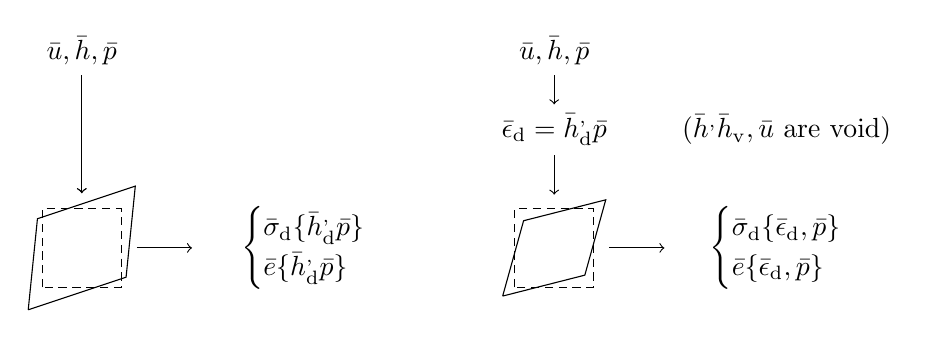
\begin{tikzpicture}[]
 \node (D) at (0,2.5) {$\bar{\ta u}, \bar{\ts h}, \bar p$};
 \draw[densely dashed] (-0.5,-0.5) rectangle (0.5,0.5);
 \draw[] (-0.679901, -0.785203) -- (0.562857, -0.370962) -- (0.679901, 0.785203) -- (-0.562857, 0.370962) -- (-0.679901, -0.785203);
 \node at (3,0) {$\begin{cases} \bar{\ts\sigma}_\dev\{\bar{\ts h}_\dev^\sym, \bar{p}\} \\ \bar{e}\{\bar{\ts h}_\dev^\sym, \bar{p}\}\end{cases}$};
 \draw[->] (D.south) -- +(0,-1.5);
 \draw[->] (D.south) -- +(0,-1.5);
 \draw[->] (0.7,0) -- (1.4,0);

 \begin{scope}[shift={(6,0)}]
 \draw[densely dashed] (-0.5,-0.5) rectangle (0.5,0.5);
 \draw[] (-0.654469, -0.611173) -- (0.388827, -0.345531) -- (0.654469, 0.611173) -- (-0.388827, 0.345531) -- (-0.654469, -0.611173);
 \node (A) at (0,2.5) {$\bar{\ta u}, \bar{\ts h}, \bar p$};
 \node (B) at (0,1.5) {$\bar{\ts \epsilon}_\dev = \bar{\ts h}_\dev^\sym, \bar{p}$};
 \node[anchor=west] at (1.5,1.5) {($\bar{\ts h}^\skw, \bar{h}_\vol, \bar{\ta u}$ are void)};
 \node at (3,0) {$\begin{cases} \bar{\ts\sigma}_\dev\{\bar{\ts\epsilon}_\dev, \bar{p}\} \\ \bar{e}\{\bar{\ts\epsilon}_\dev, \bar{p}\}\end{cases}$};
 \draw[->] (A.south) -- (B.north);
 \draw[->] (B.south) -- +(0,-0.5);
 \draw[->] (0.7,0) -- (1.4,0);
 \end{scope}
 
\end{tikzpicture}
 \caption{Comparison of the RVE-problem formulations; Original (left) and Canonical (right).}\label{fig:format_comparison}
\end{figure}
An illustrative comparison between the two RVE formulations are shown \figref{fig:format_comparison}.
Despite the different displacement fields, the homogenized responses, $\bar{\ts\sigma}_\dev$ and $\bar{e}$, are the same.

\subsection{RVE-problem -- Canonical weak format in the incompressible limit}

Fine-scale incompressibility within the RVE is defined by $\hat{e}(p)=0 \,\,\forall \ta{x}\in\Omega_\rve$, which gives  $c^*_\rve(p;\delta p)=0\,\,\forall\delta p \in \set{P}_\rve$.
As a result, $\bar{e}\epspargs=\homgen{ \hat{e}(p) }=0$, and we obtain the reduced RVE-problem: For given values $\bar{\ts\epsilon}_\dev$, $ \bar{p}$, that represent the macroscale fields, find the subscale fields $(\ta{u},p,\ta{t})\in\set{U}_\rve\times\set{P}_\rve\times\set{T}_\rve$ that solve the system
%----------------------------------------------------------------------------
\begin{subequations}\label{eq251}
\begin{alignat}{2}
    a_\rve(\ta{u},\delta\ta{u}) + b_\rve(p,\delta\ta{u}) + d_\rve(\ta{t},\delta\ta{u}) &= 0
    &\quad& \forall \delta\ta{u} \in \set{U}_\rve
\label{eq251a} \\
    b_\rve(\delta p,\ta{u}) &= 0
    &\quad& \forall \delta p \in \set{P}_\rve
\label{eq251b} \\
    d_\rve(\delta\ta{t},\ta{u}) &= d_\rve(\delta\ta{t},\bar{\ts\epsilon}_\dev \cdot[\ta{x}-\bar{\ta{x}}])
    &\quad& \forall \delta\ta{t} \in \set{T}_\rve
\label{eq251c}
\end{alignat}
\end{subequations}
%----------------------------------------------------------------------------
In practice, there is (of course) no need to establish \cref{eq251} as a separate system from \cref{eq51}, since $\bar{e}=0$ is obtained directly as part of the solution of \cref{eq51} in this case.


\section{Variational properties of the RVE-problem -- Energy bounds from RVE-functional}

\subsection{Variational properties for the canonical formulation of the RVE-problem -- The RVE-potential}

In order to establish bounds on the homogenized properties based on the results from the Dirichlet and Neumann problems, we shall introduce an appropriate ``RVE-potential'' as follows:
%----------------------------------------------------------------------------------------------------------------
\begin{equation}
    \Pi_\rve(\bar{\ts\epsilon}_\dev,\bar{p};\ta{u},p,\ta{t},\bar{e}) =
    \Lambda_\rve(\ta{u},p) + \bar{p}\,\bar{e} +
    d_\rve(\ta{t},\ta{u}-\bar{\ts\epsilon}_\dev\cdot[\ta{x}-\bar{\ta{x}}]-\bar{e}\,\ta{x}_\mean)
\label{eq81}
\end{equation}
%----------------------------------------------------------------------------------------------------------------------
where $\Lambda_\rve(\ta{u},p)$ is the ``intrinsic'' energy potential that was defined in \cref{eqRveBulkPotential}.

We now define the volume-specific ``macroscale energy density''\footnote{$\bar{\psi}_\rve \to \bar{\psi}$, the ``effective energy density'', for sufficiently large RVE. } as the value of $\Pi_\rve$ at the following generalized saddle-point:
%----------------------------------------------------------------------------------------------------------------
\begin{equation}
    \bar{\psi}_\rve\epspargs =
    \inf_{\hat{\ta{u}}\in\set{U}_\rve}
    \sup_{\substack{ \hat{p}\in\set{P}_\rve \\ \hat{\ta{t}}\in\set{T}_\rve }}
    \inf_{ \hat{\bar{e}}\in\set{R} }
    \Pi_\rve(\bar{\ts\epsilon}_\dev,\bar{p};\hat{\ta{u}},\hat{p},\hat{\ta{t}},\hat{\bar{e}})
\label{eq:periodic_energy}
\end{equation}
%----------------------------------------------------------------------------------------------------------------------
A stationary point of $\Pi_\rve$ is defined by the relations
%----------------------------------------------------------------------------
\begin{subequations}\label{eq:rveStat}
\begin{alignat}{4}
    &(\Pi_\rve)'_u(\bar{\ts\epsilon}_\dev,\bar{p};\ta{u},p,\ta{t},\bar{e};\delta\ta{u}) &&= 0
    & \quad & \forall \delta\ta{u} &&\in\set{U}_\rve
\label{eq:rveStata} \\
    &(\Pi_\rve)'_p(\bar{\ts\epsilon}_\dev,\bar{p};\ta{u},p,\ta{t},\bar{e};\delta p) &&= 0
    & \quad & \forall \delta p &&\in\set{P}_\rve
\label{eq:rveStatb} \\
    &(\Pi_\rve)'_t(\bar{\ts\epsilon}_\dev,\bar{p};\ta{u},p,\ta{t},\bar{e};\delta\ta{t}) &&= 0
    & \quad & \forall \delta\ta{t} &&\in\set{T}_\rve
\label{eq:rveStatc} \\
    &(\Pi_\rve)'_{\bar{e}}(\bar{\ts\epsilon}_\dev,\bar{p};\ta{u},p,\ta{t},\bar{e};\delta \bar{e}) &&= 0
    & \quad & \forall \delta \bar{e} &&\in\set{R}
\label{eq:rveStatd}
\end{alignat}
\end{subequations}
%----------------------------------------------------------------------------
It is readily seen that the system in \cref{eq:rveStat} is precisely that of \cref{eq51}, and we may parameterize its solution as
%----------------------------------------------------------------------------------------------------------------
\begin{equation}
    \ta{u}=\ta{u}\epspargs, \,\,
    p=p\epspargs, \,\,
    \ta{t}=\ta{t}\epspargs, \,\,
    \bar{e}=\bar{e}\epspargs
\label{eq85}
\end{equation}
%----------------------------------------------------------------------------------------------------------------------
At the stationary point, we may use the result in \cref{eq:rveStatc} to conclude that
%----------------------------------------------------------------------------------------------------------------
\begin{equation}
    d_\rve(\ta{t}\epspargs,\ta{u}\epspargs-\bar{\ts\epsilon}_\dev\cdot[\ta{x}-\bar{\ta{x}}]-\bar{e}\epspargs\,\ta{x}_\mean) = 0
\label{eq86}
\end{equation}
%----------------------------------------------------------------------------------------------------------------------
whereby the energy at the stationary point is deduced to become
%----------------------------------------------------------------------------------------------------------------
\begin{equation}
    \bar{\psi}_\rve\epspargs =
    \Lambda_\rve(\ta{u}\epspargs,p\epspargs) + \bar{p}\,\bar{e}\epspargs
\label{eq87}
\end{equation}
%----------------------------------------------------------------------------------------------------------------------
We now deduce that $\bar{\psi}_\rve$ serves as the ``macroscale energy density'' for $\bar{\ts\sigma}_\dev$ and $\bar{e}$ in the sense that we have the macroscale constitutive relations
%----------------------------------------------------------------------------------------------------------------
\begin{equation}
    \bar{\ts\sigma}_\dev\epspargs = \frac{\partial \bar{\psi}_\rve\epspargs}{\partial \bar{\ts\epsilon}_\dev}, \quad
     \bar{e}\epspargs = \frac{\partial \bar{\psi}_\rve\epspargs}{\partial \bar{p}}
\label{eq88}
\end{equation}
%----------------------------------------------------------------------------------------------------------------------
Details of the proof are given in \appref{appendix:macroEnergy}.

From the solution of the RVE-problem, $\bar{e}$ is obtained directly as a primary variable.
The deviatoric stress $\bar{\ts\sigma}_\dev$ is obtained by post-processing:
\begin{align}
 \bar{\ts\sigma}_\dev = \homgen{\ts\sigma_\dev} = \frac{1}{\volume} \int_{\Gamma_\rve^+} \ta t \outerp \jmp{\ta x - \bar{\ta x}}\dif S + \bar{p}\ts I
\label{eq:weak_periodic_sigma_dev}
\end{align}


\subsection{Variational properties for Dirichlet boundary conditions}

In order to establish a suitable variational setting we replace the solution space $\set{U}_\rve$ with $\set{U}_\rve^\Dirichlet\subseteq\set{U}_\rve$ defined as
%----------------------------------------------------------------------------
\begin{align}
    \set{U}_\rve^\Dirichlet &= \{\ta{v} \,|\,\, \ta{v}=\check{\ts\epsilon}_\dev\cdot[\ta{x}-\bar{\ta{x}}]+\check{e}\,\ta{x}_\mean+\ta{v}^\fluct, (\check{\ts\epsilon}_\dev,\check{e}, \ta v^\fluct)\in\set{R}^{3\times3}_\dev \times\set{R}\times\set{U}_\rve^{\Dirichlet,\fluct} \}
\label{eq61a} \\
\intertext{where}
    \set{U}_\rve^{\Dirichlet,\fluct} &= \{\ta{v}\in \set{U}_\rve^\fluct \,|\,\, \ta{v}=\ta{0} \text{ on } \Gamma_\rve \}
\label{eq61b}
\end{align}
%----------------------------------------------------------------------------
while $\set{P}_\rve^\Dirichlet=\set{P}_\rve$, ${\set{T}}_\rve^\Dirichlet={\set{T}}_\rve$ are the same spaces as for the generic problem.
The generalized saddle-point problem \cref{eq:periodic_energy} can now be rephrased as
%----------------------------------------------------------------------------------------------------------------
\begin{equation}
    \bar{\psi}_\rve^\Dirichlet\epspargs =
    \inf_{\substack{
    \hat{\ta{u}}^\fluct\in\set{U}_\rve^{\Dirichlet,\fluct}\\
    \check{\ts\epsilon}_\dev\in \set{R}^{3\times 3}_\dev \\
    \check{e}\in\set{R}
    }}
    \sup_{\substack{
    \hat{p}\in\set{P}_\rve\\
    \hat{\ta{t}}\in\set{T}_\rve
    }}
    \inf_{
    \hat{\bar{e}}\in\set{R}
    }
    \Pi_\rve(\bar{\ts\epsilon}_\dev,\bar{p};\check{\ts\epsilon}_\dev\cdot[\ta{x}-\bar{\ta{x}}] + \check{e}\,\ta{x}_\mean+\hat{\ta{u}}^\fluct,\hat{p},\hat{\ta{t}},\hat{\bar{e}})
\label{eq:dirichlet_energy}
\end{equation}
%----------------------------------------------------------------------------------------------------------------------
where
%----------------------------------------------------------------------------------------------------------------
\begin{multline}
    \Pi_\rve(\bar{\ts\epsilon}_\dev,\bar{p};\check{\ts\epsilon}_\dev\cdot[\ta{x}-\bar{\ta{x}}] + \check{e}\,\ta{x}_\mean+\hat{\ta{u}}^\fluct,\hat{p},\hat{\ta{t}},\hat{\bar{e}}) =
\\
    \Lambda_\rve(\check{\ts\epsilon}_\dev\cdot[\ta{x}-\bar{\ta{x}}] + \check{e}\,\ta{x}_\mean+\hat{\ta{u}}^\fluct,\hat{p}) + \bar{p}\,\hat{\bar{e}}
     + d_\rve(\hat{\ta{t}}, [\check{\ts\epsilon}_\dev-\bar{\ts\epsilon}_\dev]\cdot[\ta{x}-\bar{\ta{x}}]+[\check{e}-\hat{\bar{e}}]\,\ta{x}_\mean)
\label{eq91b}
\end{multline}
%----------------------------------------------------------------------------------------------------------------------
The only possibility to obtain a finite value of $\bar{\psi}_\rve^\Dirichlet$ while evaluating the sup over $\hat{\ta{t}}\in\set{T}_\rve$ is to set $\check{\ts\epsilon}_\dev = \bar{\ts\epsilon}_\dev$ and $\check{e} = \hat{\bar{e}}$.
Hence, we replace the saddle-point problem by
%----------------------------------------------------------------------------------------------------------------
\begin{equation}
    \bar{\psi}_\rve^\Dirichlet\epspargs =
    \inf_{
    \hat{\ta{u}}^\fluct\in\set{U}_\rve^{\Dirichlet,\fluct}
    }
    \sup_{
    \hat{p}\in\set{P}_\rve
    }
    \inf_{
    \hat{\bar{e}}\in\set{R}
    }
    \Pi_\rve^\Dirichlet(\bar{\ts\epsilon}_\dev,\bar{p};\hat{\ta{u}}^\fluct,\hat{p},\hat{\bar{e}})
\label{eq93a}
\end{equation}
%----------------------------------------------------------------------------------------------------------------------
where
%----------------------------------------------------------------------------------------------------------------
\begin{equation}
    \Pi_\rve^\Dirichlet(\bar{\ts\epsilon}_\dev,\bar{p};\hat{\ta{u}}^\fluct,\hat{p},\hat{\bar{e}})
    = \Lambda_\rve(\bar{\ts\epsilon}_\dev\cdot[\ta{x}-\bar{\ta{x}}]+\hat{\bar{e}}\,\ta{x}_\mean+\hat{\ta{u}}^\fluct,\hat{p}) - \bar{p}\,\hat{\bar{e}}
\label{eq93b}
\end{equation}
%----------------------------------------------------------------------------------------------------------------------
A stationary point of $\Pi_\rve^\Dirichlet$ is defined by the relations
%----------------------------------------------------------------------------
\begin{subequations}\label{eq94}
\begin{alignat}{4}
    &(\Pi_\rve^\Dirichlet)'_u(\bar{\ts\epsilon}_\dev,\bar{p};\ta{u}^\fluct,p,\bar{e};\delta\ta{u}^\fluct) &&= 0
    &\quad & \forall \delta\ta{u}^\fluct &&\in\set{U}_\rve^{\Dirichlet,\fluct}
\label{eq94a} \\
    &(\Pi_\rve^\Dirichlet)'_p(\bar{\ts\epsilon}_\dev,\bar{p};\ta{u}^\fluct,p,\bar{e};\delta p) &&= 0
    &\quad & \forall \delta p &&\in\set{P}_\rve
\label{eq94b} \\
    &(\Pi_\rve^\Dirichlet)'_{\bar{e}}(\bar{\ts\epsilon}_\dev,\bar{p};\ta{u}^\fluct,p,\ta{t},\bar{e};\delta\bar{e}) &&= 0
    &\quad & \forall \delta\bar{e} &&\in\set{R}
\label{eq94c}
\end{alignat}
\end{subequations}
%----------------------------------------------------------------------------
and this system of equations takes the explicit form: For given values $\bar{\ts\epsilon}_\dev, \bar{p}$, find the subscale fields $(\ta{u}^\fluct,p,\bar{e})\in\set{U}_\rve^{\Dirichlet,\fluct}\times\set{P}_\rve\times\set{R}$ that solve the system
%----------------------------------------------------------------------------
\begin{subequations}\label{eq:weak_form_dirichlet}
\begin{alignat}{2}
    a_\rve(\bar{\ts\epsilon}_\dev\cdot[\ta{x}-\bar{\ta{x}}]+\ta{u}^\fluct;\delta\ta{u}^\fluct) + b_\rve(p,\delta\ta{u}^\fluct) &= 0
    &\quad& \forall \delta\ta{u}^\fluct \in \set{U}_\rve^{\Dirichlet,\fluct}
\label{eq64a} \\
    b_\rve(\delta p,\ta{u}^\fluct) + b_\rve(\delta p,\bar{e}\,\ta{x}_\mean) + c^*_\rve(p;\delta p) &= 0
    &\quad& \forall \delta p \in \set{P}_\rve
\label{eq64b} \\
    b_\rve(p,\delta\bar{e}\,\ta{x}_\mean) &=
    - \bar{p}\,\delta\bar{e}
    &\quad& \forall \delta\bar{e} \in \set{R}
\label{eq64c}
\end{alignat}
\end{subequations}
%----------------------------------------------------------------------------
Finally, the macroscale energy density at the stationary point becomes
%----------------------------------------------------------------------------------------------------------------
\begin{equation}
    \bar{\psi}_\rve^\Dirichlet\epspargs =
    \Lambda_\rve(\bar{\ts\epsilon}_\dev\cdot[\ta{x}-\bar{\ta{x}}]+\bar{e}\epspargs\,\ta{x}_\mean+\ta{u}^\fluct\epspargs,p\epspargs) +\bar{p}\,\bar{e}\epspargs
\label{eq95}
\end{equation}
%----------------------------------------------------------------------------------------------------------------------

From the RVE-problem in \cref{eq:weak_form_dirichlet}, $\bar{e}$ is obtained directly as a primary variable.
The deviatoric stress $\bar{\ts\sigma}_\dev$ is obtained by post-processing:
\begin{align}
 \bar{\ts\sigma}_\dev = \homgen{\ts\sigma_\dev} = \frac{1}{\volume} \int_{\Gamma_\rve^+} \ta t \outerp \jmp{\ta x - \bar{\ta x}}\dif S + \bar{p}\ts I
\label{eq:weak_dirichlet_sigma_dev}
\end{align}
However in practice $\bar{\ts\sigma}_\dev$ is conveniently obtained as the reaction forces associated with the prescribed $\bar{\ts\epsilon}_\dev$.

\textbf{Remark}:
The VMCM in \cref{eq:macro_homogeneity_original} is still valid for the restricted space $\set{U}_\rve^{\Dirichlet,\fluct}\subset \set{U}_\rve^\fluct$.
Since $d_\rve(\delta\ta t^\fluct, \ta u^\fluct) = 0\;\forall\,\ta u^\fluct \in \set U_\rve^{\Dirichlet,\fluct}$, \cref{eq:macro_homogeneity_original_a} is satisfied for all $\delta\ta u^\fluct\in\set U^{\Dirichlet,\fluct}$. $\Box$

\subsection{Variational properties for Neumann boundary conditions}
The Neumann condition represents the weakest possible way of enforcing the micro-periodicity condition.
Here it is considered as a \emph{model assumption}; however, it is also possible to view this choice as a (crude) FE-approximation of the deviatoric traction field.
The pertinent RVE-problem is obtained from the general format upon restricting the space $\set{T}_\rve$, i.e.\ introducing $\set{T}_\rve^\Neumann\subseteq\set{T}_\rve$ defined as
%----------------------------------------------------------------------------
\begin{equation}
    \set{T}_\rve^\Neumann =
    \{\ta{t}\in\set{T}_\rve\,|\,\, \exists(\check{\ts\sigma}_\dev,\check{p})\in\set{R}^{3\times3}_\dev \times\set{R} \text{ s.t. }
    \ta{t}=\left[\check{\ts\sigma}_\dev-\check{p}\ts{I}\right]\cdot\ta{n} \text{ on } \Gamma_\rve^+\}
    \label{eq65}
\end{equation}
%---------------------------------------------------------------------------
while $\set{U}_\rve^\Neumann=\set{U}_\rve$ and $\set{P}_\rve^\Neumann=\set{P}_\rve$ are left unrestricted.
Clearly, the choice of $\set{T}_\rve^\Neumann$ restricts the tractions to become piecewise constant on each of the three positive boundary faces of the RVE-cube.
The generalized saddle-point problem \cref{eq:periodic_energy} can then be rephrased as
%----------------------------------------------------------------------------------------------------------------
\begin{equation}
    \bar{\psi}_\rve^\Neumann\epspargs =
    \inf_{
    \hat{\ta{u}}\in\set{U}_\rve
    }
    \sup_{\substack{
    \hat{p}\in\set{P}_\rve \\
    \check{\ts\sigma}_\dev\in\set{R}^{3\times3}_\dev \\
    \check{p}\in\set{R}
    }}
    \inf_{
    \hat{\bar{e}}\in\set{R}
    }
    \Pi_\rve(\bar{\ts\epsilon}_\dev,\bar{p};\hat{\ta{u}},\hat{p},\left[\check{\ts\sigma}_\dev-\check{p}\ts{I}\right]\cdot\ta{n},\hat{\bar{e}})
\label{eq:neumann_energy}
\end{equation}
%----------------------------------------------------------------------------------------------------------------------
where
%----------------------------------------------------------------------------------------------------------------
\begin{multline}
    \Pi_\rve(\bar{\ts\epsilon}_\dev,\bar{p};\hat{\ta{u}},\hat{p},\left[\check{\ts\sigma}_\dev-\check{p}\ts{I}\right]\cdot\ta{n},\hat{\bar{e}})
    =
\\
    \Lambda_\rve(\hat{\ta{u}},\hat{p}) + \bar{p}\,\hat{\bar{e}} +
    d_\rve(\left[\check{\ts\sigma}_\dev-\check{p}\ts{I}\right]\cdot\ta{n},\hat{\ta{u}}-\bar{\ts\epsilon}_\dev\cdot
    [\ta{x}-\bar{\ta{x}}]-\hat{\bar{e}}\,\ta{x}_\mean)
\label{eq96b}
\end{multline}
%----------------------------------------------------------------------------------------------------------------------
The only possibility to obtain a finite value of $\bar{\psi}_\rve^\Neumann$ while evaluating the $\inf$ over $\hat{\bar{e}}\in\set{R}$ is to set $\check{p} = \bar{p}$.
As a direct consequence the variable $\hat{\bar{e}}$ disappears in the resulting expression, cf.\ \cref{eq98b} below.
Moreover, from \cref{eq:weak_periodic_sigma_dev} we see that for tractions $\ta t \in \set T_\rve^\Neumann$ we obtain $\check{\ts\sigma}_\dev
= \homgen{ \hat{\ts{\sigma}}_\dev(\ts{\epsilon}_\dev[\ta{u}\epspargs]) } = \bar{\ts\sigma}_\dev\epspargs$.
%----------------------------------------------------------------------------------------------------------------------
Hence, we replace the saddle-point problem by
%----------------------------------------------------------------------------------------------------------------
\begin{align}
    \bar{\psi}_\rve^\Neumann\epspargs =
    \inf_{
    \hat{\ta{u}}\in\set{U}_\rve
    }
    \sup_{\substack{
    \hat{p}\in\set{P}_\rve \\
    \bar{\ts\sigma}_\dev\in\set{R}^{3\times3}_\dev
    }}
    \Pi_\rve^\Neumann(\bar{\ts\epsilon}_\dev,\bar{p};\hat{\ta{u}},\hat{p},\bar{\ts\sigma}_\dev)
%\nonumber \\
%    &=& \inf_{\tilde{\ta{u}}^\fluct\in\set{U}^{\Dirichlet,\fluct}} \sup_{\tilde{p}\in\set{P} \tilde{\ta{t}}\in\set{T}} \inf_{\check{e}\in\set{R}}
%    \left[\Lambda_\rve(\tilde{\ta{u}},\tilde{p}) - \bar{p}\,\check{e}\right]
\label{eq98a}
\end{align}
%----------------------------------------------------------------------------------------------------------------------
where
%----------------------------------------------------------------------------------------------------------------
\begin{equation}
    \Pi_\rve^\Neumann(\bar{\ts\epsilon}_\dev,\bar{p};\hat{\ta{u}},\hat{p},\bar{\ts\sigma}_\dev)
    = \Lambda_\rve(\hat{\ta{u}},\hat{p}) +
    d_\rve([\bar{\ts\sigma}_\dev-\bar{p}\ts{I}]\cdot\ta n,\hat{\ta{u}}-\bar{\ts\epsilon}_\dev\cdot[\ta{x}-\bar{\ta{x}}])
\label{eq98b}
\end{equation}
%----------------------------------------------------------------------------------------------------------------------
A stationary point of $\Pi_\rve^\Neumann$ is defined by the relations
%----------------------------------------------------------------------------
\begin{subequations}\label{eq104}
\begin{alignat}{4}
    &(\Pi_\rve^\Neumann)'_u(\bar{\ts\epsilon}_\dev,\bar{p};\ta{u},p,\bar{\ts\sigma}_\dev;\delta\ta{u}) &&= 0
    &\quad & \forall \delta\ta{u} &&\in\set{U}_\rve
\label{eq104a} \\
    &(\Pi_\rve^\Neumann)'_p(\bar{\ts\epsilon}_\dev,\bar{p};\ta{u},p,\bar{\ts\sigma}_\dev;\delta p) &&= 0
    &\quad & \forall \delta p &&\in\set{P}_\rve
\label{eq104b} \\
    &(\Pi_\rve^\Neumann)'_{\bar{\sigma}}(\bar{\ts\epsilon}_\dev,\bar{p};\ta{u},p,\bar{\ts\sigma}_\dev;\delta\bar{\ts\sigma}_\dev) &&= 0
    &\quad & \forall \delta\bar{\ts\sigma}_\dev &&\in\set{R}^{3\times3}_\dev
\label{eq104c}
\end{alignat}
\end{subequations}
%----------------------------------------------------------------------------
and this system of equations takes the explicit form: For given values $\bar{\ts\epsilon}_\dev, \bar{p}$, find the subscale fields $\ta{u},p,\bar{\ts\sigma}_\dev\in\set{U}_\rve\times\set{P}_\rve\times\set{R}^{3\times 3}_\dev$ that solve the system
%----------------------------------------------------------------------------
\begin{subequations}\label{eq67}
\begin{alignat}{2}
    a_\rve(\ta{u};\delta\ta{u}) + b_\rve(p,\delta\ta{u}) +  d_\rve(\bar{\ts\sigma}_\dev\cdot\ta n,\delta\ta{u}) &= d_\rve(\bar{p}\,\ta n,\delta\ta u)
    && \quad\forall \delta\ta{u} \in \set{U}_\rve\hspace{-2em}
\label{eq67a} \\
    b_\rve(\delta p,\ta{u}) + c^*_\rve(p;\delta p) &= 0
    && \quad\forall \delta p \in \set{P}_\rve\hspace{-2em}
\label{eq67b} \\
    d_\rve(\delta\bar{\ts\sigma}_\dev\cdot\ta n,\ta{u}) &= - \bar{\ts\epsilon}_\dev\dprod\delta\bar{\ts\sigma}_\dev
    && \quad\forall \delta\bar{\ts\sigma}_\dev \in\set{R}^{3\times3}_\dev\hspace{-2em}
\label{eq67c}
\end{alignat}
\end{subequations}
%----------------------------------------------------------------------------
Finally, we obtain the macroscale energy density as
%----------------------------------------------------------------------------------------------------------------
\begin{equation}
    \bar{\psi}_\rve^\Neumann\epspargs =
    \Lambda_\rve(\ta{u}\epspargs,p\epspargs) + \bar{p}\,\homgen{ \ta{u}\epspargs\cdot\diff }
\label{eq105}
\end{equation}
%----------------------------------------------------------------------------------------------------------------------

From the RVE-problem in \cref{eq67}, $\bar{\ts\sigma}_\dev$ is obtained directly as a primary variable.
The volumetric strain $\bar{e}$ is obtained by post-processing:
\begin{align}
 \bar{e} = \homgen{\ta u\cdot\diff} = \frac{1}{\volume} \int_{\Gamma_\rve} \ta u \cdot \ta n\dif S.
\end{align}

\textbf{Remark}:
The VMCM in \cref{eq:macro_homogeneity_original} is still valid for the restricted space $\set{T}_\rve^\fluct = \{\ta 0\}$.
Since $d_\rve(\ta 0, \bullet) = 0$, \cref{eq:macro_homogeneity_original_a} is valid for all $\delta\ta u^\fluct \in \set U_\rve^\fluct$. $\Box$


\subsection{Macroscale tangent relations}
In order to solve the (generally nonlinear) macroscale problem \cref{eq17} in the FE\textsuperscript{2}-setting using Newton iterations, we need the pertinent tangent operators.
Linearizing the implicit relations $\bar{\ts\sigma}_\dev\epspargs$ and $\bar{e}\epspargs$ we obtain
\begin{align}
 \dif\bar{\ts\sigma}_\dev = \bar{\tf E} \dprod \dif\bar{\ts\epsilon}_\dev + \bar{\ts E}\, \dif\bar{p},
\quad
 \dif\bar{e} = \bar{\ts C} \dprod \dif\bar{\ts\epsilon}_\dev - \bar{C}\, \dif\bar{p}
\label{eq:periodic_difsigma}
\end{align}
thereby defining the tangents $\bar{\tf E}$ (4th order), $\bar{\ts E}$ (2nd order), $\bar{\ts C}$ (2nd order), and $\bar{C}$ (scalar).
Since a potential exists, it follows that $\bar{\tf {E}}$ possesses major symmetry and that $\bar{\ts E} = \bar{\ts C}$, cf.\ \"Ohman et. al \cite{ohman_computational_2012}.

In order to compute the tangent operators, it is necessary to first compute the relevant sensitivity fields w.r.t.\ changes of the macroscale variables $\bar{\ts\epsilon}_\dev$ and $\bar{p}$, and they are solved from the pertinent tangent problem.
On should then note that the particular sensitivity fields that are actually exploited (and needed) and the corresponding explicit formulation of the tangent problem depend on the chosen formulation of the RVE-problem (in terms of the boundary conditions: Weakly Periodic, Dirichlet, Neumann). 
Here, we shall give details only on the ``generic'' choice of the weakly periodic conditions.

\textbf{Remark}: In the case of macroscale incompressibility, $\bar{\ts C}$ and $\bar{C}$ will vanish. $\Box$

As a point of departure for computing the tangent tensors, we note that $\bar{e}\epspargs$ is a primary variable in the RVE-problem, whereas $\bar{\ts\sigma}_\dev\epspargs$ is post-processed via \cref{eq:weak_periodic_sigma_dev}.
We thus need to compute sensitivities of $\bar{e}$ and $\ta t$ from the tangent problem.
To begin with, we establish the linearized form of \cref{eq51} at the solution state to obtain
\begin{subequations}
\begin{alignat}{2}
    (a_\rve)'(\ta{u};\delta\ta{u},\dif\ta u) + b_\rve(\dif p,\delta\ta{u}) + d_\rve(\dif\ta{t},\delta\ta{u}) &= 0
    &\quad& \forall \delta\ta{u} \in \set{U}_\rve
\\
    b_\rve(\delta p,\dif\ta{u}) + (c^*_\rve)'(p;\delta p, \dif p) &= 0
    &\quad& \forall \delta p \in \set{P}_\rve
\\
    d_\rve(\delta\ta{t},\dif\ta{u}) - d_\rve(\delta\ta{t},\dif\bar{e}\,\ta{x}_\mean) = d_\rve(\delta\ta{t},\dif\bar{\ts\epsilon}_\dev \cdot[\ta{x}&-\bar{\ta{x}}])
    &\quad& \forall \delta\ta{t} \in \set{T}_\rve
\\
    - d_\rve(\dif\ta{t},\delta\bar{e}\,\ta{x}_\mean) &= - \dif\bar{p}\,\delta\bar{e}
    &\quad& \forall \delta\bar{e} \in \set{R}
\end{alignat}
\end{subequations}
which must be valid for any given perturbations $\dif\bar{\ts\epsilon}_\dev$ and $\dif\bar{p}$ giving rize to the corresponding perturbations $\dif\ta u$, $\dif p$, $\dif\ta t$, and $\dif\bar{e}$ in the solution fields.

Next, we introduce orthonormal base dyads $\ts G_i$, $i = 1,2,...,8$ to ensure that the deviatoric tensors $\ts\epsilon_\dev$ and $\ts\sigma_\dev$ are, indeed, deviatoric in character.
In other words we do not use the conventional base dyads $\ta e_i\outerp\ta e_j$, $i,j=1,2,3$, but we rather introduce the new set of base dyads such that the requirement $\ts G_i \dprod \ta I = 0$ for $i=1,2,...,8$ is fulfilled.
Examples of such (generally unsymmetric) dyads with Cartesian components, are
\begin{equation}
\begin{gathered}
 \ts G_1 = \frac{1}{\sqrt{6}}\left[\begin{smallmatrix} 2 & 0 & 0\\ 0 & -1 & 0\\ 0 & 0 & -1\end{smallmatrix}\right],\;
 \ts G_2 = \left[\begin{smallmatrix} 0 & 0 & 0\\ 0 & 1 & 0 \\ 0 & 0 & -1\end{smallmatrix}\right],\;
 \ts G_3 = \left[\begin{smallmatrix} 0 & 1 & 0\\ 0 & 0 & 0 \\ 0 & 0 & 0\end{smallmatrix}\right],\;
 \ldots,\;
 \ts G_8 = \left[\begin{smallmatrix} 0 & 0 & 0\\ 0 & 0 & 0 \\ 0 & 1 & 0\end{smallmatrix}\right].
\end{gathered}
\end{equation}
with respect to this basis, we have the representation
\begin{gather}
 \ts\epsilon_\dev = \sum_k (\ts\epsilon_\dev)_k \, \ts G_k,\quad 
 (\ts\epsilon_\dev)_k = \ts G_k \dprod \ts\epsilon_\dev
\\
 \ts\sigma_\dev = \sum_k (\ts\sigma_\dev)_k \, \ts G_k,\quad
 (\ts\sigma_\dev)_k = \ts G_k \dprod \ts\sigma_\dev
\end{gather}
% Hence, the component form of \cref{eq:periodic_difsigma} becomes
% \begin{align}
%  (\dif\ts\sigma_\dev)_i = \sum_k (\bar{\tf E})_{ik} (\dif\bar{\ts\epsilon}_\dev)_k + (\bar{\ts E})_i\dif\bar{p}
% \end{align}
% and
% \todo{why for E but not C}
% \begin{align}
%  \bar{\tf E} = \sum_{i,j} (\bar{\tf E})_{ij} \ts G_i \outerp \ts G_j,\quad \bar{\ts E} = \sum_i (\bar{\ts E})_i \ts G_i
% \end{align}
Next, we express the pertinent sensitivities via the representations
\begin{subequations}
\begin{align}
 \dif\ta u &= \sum_k \ta u_\ded^{(k)} (\dif\bar{\ts\epsilon}_\dev)_k + \ta u_\dep\,\dif\bar{p}
\\
 \dif p &= \sum_k p_\ded^{(k)} (\dif\bar{\ts\epsilon}_\dev)_k + p_\dep\,\dif\bar{p}
\\
 \dif\ta t &= \sum_k \ta t_\ded^{(k)} (\dif\bar{\ts\epsilon}_\dev)_k + \ta t_\dep\,\dif\bar{p}
\label{eq:periodic_dif_t}
\\
 \dif\bar{e} &= \sum_k \bar{e}_\ded^{(k)} (\dif\bar{\ts\epsilon}_\dev)_k + \bar{e}_\dep\,\dif\bar{p}
\label{eq:periodic_dif_ebar}
\end{align}
\end{subequations}
We thus obtain the following sets of tangent problems:
\begin{itemize}
 \item $\dif\bar{\ts\epsilon}_\dev = \ts G_k$ while $\dif\bar{p} = 0$: For $k = 1, \ldots, 8$, solve for the sensitivities $\ta{u}_\ded^{(k)}$, $p_\ded^{(k)}$, $\ta{t}_{\ded}^{(k)}$, $\bar{e}_\ded^{(k)}$ from the system 
\end{itemize}
\begin{subequations}\label{eq:p_sensitivities_d}
\begin{alignat}{2}
    (a_\rve)'(\ta{u};\delta\ta{u},\ta{u}_\ded^{(k)}) + b_\rve(p_\ded^{(k)},\delta\ta{u}) + d_\rve(\ta{t}_{\ded}^{(k)},\delta\ta{u}) &= 0
    &\;\;& \forall \delta\ta{u} \in \set{U}_\rve
\\
    b_\rve(\delta p,\ta{u}_\ded^{(k)}) + (c^*_\rve)'(p;\delta p, p_\ded^{(k)}) &= 0
    &\;\;& \forall \delta p \in \set{P}_\rve
\\
    d_\rve(\delta\ta{t},\ta{u}_\ded^{(k)}) - d_\rve(\delta\ta{t},\bar{e}_\ded^{(k)}\,\ta{x}_\mean) = d_\rve(\delta\ta{t}, \ts G_k \cdot[\ta{x}&-\bar{\ta{x}}])
    &\;\;& \forall \delta\ta{t} \in \set{T}_\rve
\\
    - d_\rve(\ta{t}_{\ded}^{(k)},\delta\bar{e}\,\ta{x}_\mean) &= 0
    &\;\;& \forall \delta\bar{e} \in \set{R}
\end{alignat}
\end{subequations}
\begin{itemize}
\item $\dif\bar{p} = 1$ while $\dif\bar{\ts\epsilon}_\dev = \ts 0$: Solve for the sensitivities $\ta{u}_\dep$, $p_\dep$, $\ta{t}_\dep$, $\bar{e}_\dep$ from the system 
\end{itemize}
\begin{subequations}\label{eq:p_sensitivities_p}
\begin{alignat}{2}
    (a_\rve)'(\ta{u};\delta\ta{u},\ta{u}_\dep) + b_\rve(p_\dep,\delta\ta{u}) + d_\rve(\ta{t}_\dep,\delta\ta{u}) &= 0
    &\quad& \forall \delta\ta{u} \in \set{U}_\rve
\\
    b_\rve(\delta p,\ta{u}_\dep) + (c^*_\rve)'(p;\delta p, p_\dep) &= 0
    &\quad& \forall \delta p \in \set{P}_\rve
\\
    d_\rve(\delta\ta{t},\ta{u}_\dep) - d_\rve(\delta\ta{t},\bar{e}_\dep\,\ta{x}_\mean) &= 0
    &\quad& \forall \delta\ta{t} \in \set{T}_\rve
\\
    - d_\rve(\ta{t}_\dep,\delta\bar{e}\,\ta{x}_\mean) &=
    - \delta\bar{e}
    &\quad& \forall \delta\bar{e} \in \set{R}
\end{alignat}
\end{subequations}
Now, upon linearizing \cref{eq:weak_periodic_sigma_dev} and using the representation for $\dif\ta t$ in \cref{eq:periodic_dif_t}, we obtain
\begin{align}
    \dif\bar{\ts\sigma}_{\dev}
    & =
    \frac{1}{\volume} \int_{\Gamma_\Box^+} \dif\ts t \outerp \jmp{\ta x - \bar{\ta x}}\dif S + \dif\bar{p}\ts I
\\
    &= 
    \underbrace{\sum_k \frac{1}{\volume} \int_{\Gamma_\Box^+} \ts t_\ded^{(k)} \outerp \jmp{\ta x - \bar{\ta x}}\dif S\outerp \ts G_k}_{\bar{\tf E}}\dprod\dif\bar{\ts\epsilon}_\dev
\nonumber\\
    &\phantom{=} + 
    \underbrace{\left[\frac{1}{\volume} \int_{\Gamma_\Box^+} \ts t_\dep \outerp \jmp{\ta x - \bar{\ta x}}\dif S + \ts I \right]}_{\bar{\ts E}}\dif\bar{p}
\end{align}
Directly from \cref{eq:periodic_dif_ebar}, we obtain
\begin{align}
 \dif\bar{e} = \underbrace{\sum_k \bar{e}_\ded^{(k)}\, \ts G_k}_{\bar{\ts C}} \dprod \dif \bar{\ts\epsilon}_\dev + \underbrace{\bar{e}_\dep}_{-\bar{C}}\,\dif\bar{p}
\end{align}

Macroscale tangent relations for the Dirichlet and Neumann boundary conditions are detailed in \appref{appendix:sensitivity}.

\subsection{Bounds on the macroscale energy density}

Since we have derived the Dirichlet and Neumann problems by respectively restricting the solution spaces as
\begin{align}
 \set{U}_\rve^\Dirichlet \subset \set{U}_\rve,\quad \set{T}_\rve^\Neumann \subset \set{T}_\rve
\end{align}
it follows from \cref{eq:dirichlet_energy}, \cref{eq:neumann_energy}, and \cref{eq:periodic_energy} that
\begin{align}
 \bar\psi^\Dirichlet_\rve\{\bar{\ts\epsilon}_\dev, \bar{p}\} \geq \bar\psi\{\bar{\ts\epsilon}_\dev, \bar {p}\} \geq \bar\psi^\Neumann\{\bar{\ts\epsilon}_\dev, \bar {p}\}.
\end{align}
In other words, the Dirichlet and Neumann boundary conditions represent upper and lower bounds
on the macroscale energy density that is obtained with periodic boundary conditions for any given realization of the RVE and for a given macroscale state $(\bar{\ts\epsilon}_\dev, \bar{p})$.
We note that choosing any discretization of $\set{T}_\rve$ in \cref{eq:periodic_energy} leads to a lower bound of $\bar{\psi}\epspargs$.

In the case of linear elasticity, the tangent operators represent the upscaled (=homogenized) constant operators in the representations
\begin{align}
 \bar{\ts\sigma}_\dev = \bar{\tf E} \dprod \bar{\ts\epsilon}_\dev + \bar{\ts E}\, \bar{p}, \quad \bar{e} = \bar{\ts C}\dprod\bar{\ts\epsilon}_\dev - \bar{C}\,\bar{p}
\end{align}
whereby we obtain
\begin{multline}
 \bar{\psi}_\rve\{\bar{\ts\epsilon}_\dev, \bar{p}\} = \frac12 \bar{\ts\epsilon}_\dev \dprod \bar{\tf E}\dprod \bar{\ts\epsilon}_\dev -\frac12 \bar{p}\;\bar{C}\;\bar{p}
\quad\forall\;\bar{\ts\epsilon}_\dev,\,\bar{p}
\implies
\\
 \bar{\tf E}^\Dirichlet \geq \bar{\tf E} \geq \bar{\tf E}^\Neumann,\quad
 \bar{C}^\Dirichlet \leq \bar{C} \leq \bar{C}^\Neumann
\end{multline}



\section{Numerical results}
\subsection{Preliminaries}
Computations were carried out for a random composite with spherical particles embedded in a matrix, whereby both constituents are assumed to be homogeneous and isotropic linear elastic.
The intrinsic properties are thus defined by the free energy expressions
\begin{align}
 \psi_\mathrm{u}(\ts\epsilon_\dev) = G |\ts\epsilon_\dev|^2,\quad \psi^*_{\mathrm{p}} = -\frac12 C\, p^2
\end{align}
where $G$ and $C$ ($=K^{-1}$) are the shear stiffness and bulk compliance respectively.
This choice corresponds to the standard relations
$\hat{\ts\sigma}_\dev(\ts\epsilon_\dev) = 2 G\,\ts\epsilon_\dev$ and $\hat{e}(p) = -C\, p$.
The parameter set associated with the matrix and particles are $(G_\mathrm{mat},C_\mathrm{mat})$ and $(G_\mathrm{part},C_\mathrm{part})$, respectively.

All computational results were obtained for cubic Statistical Volume Elements (SVE:s).
The target volume fraction of particles if 10\% and their size-distribution, in terms of diameter, is uniform in the range $[\frac23 ,\frac43]$, thus with a mean value of $1$.
Two examples of realizations with SVE-size $L_\rve = 6$ and $L_\rve = 9$ are shown in \figref{fig:rve_sample6,fig:rve_sample9}, respectively.

\begin{figure}[H]
\centering
 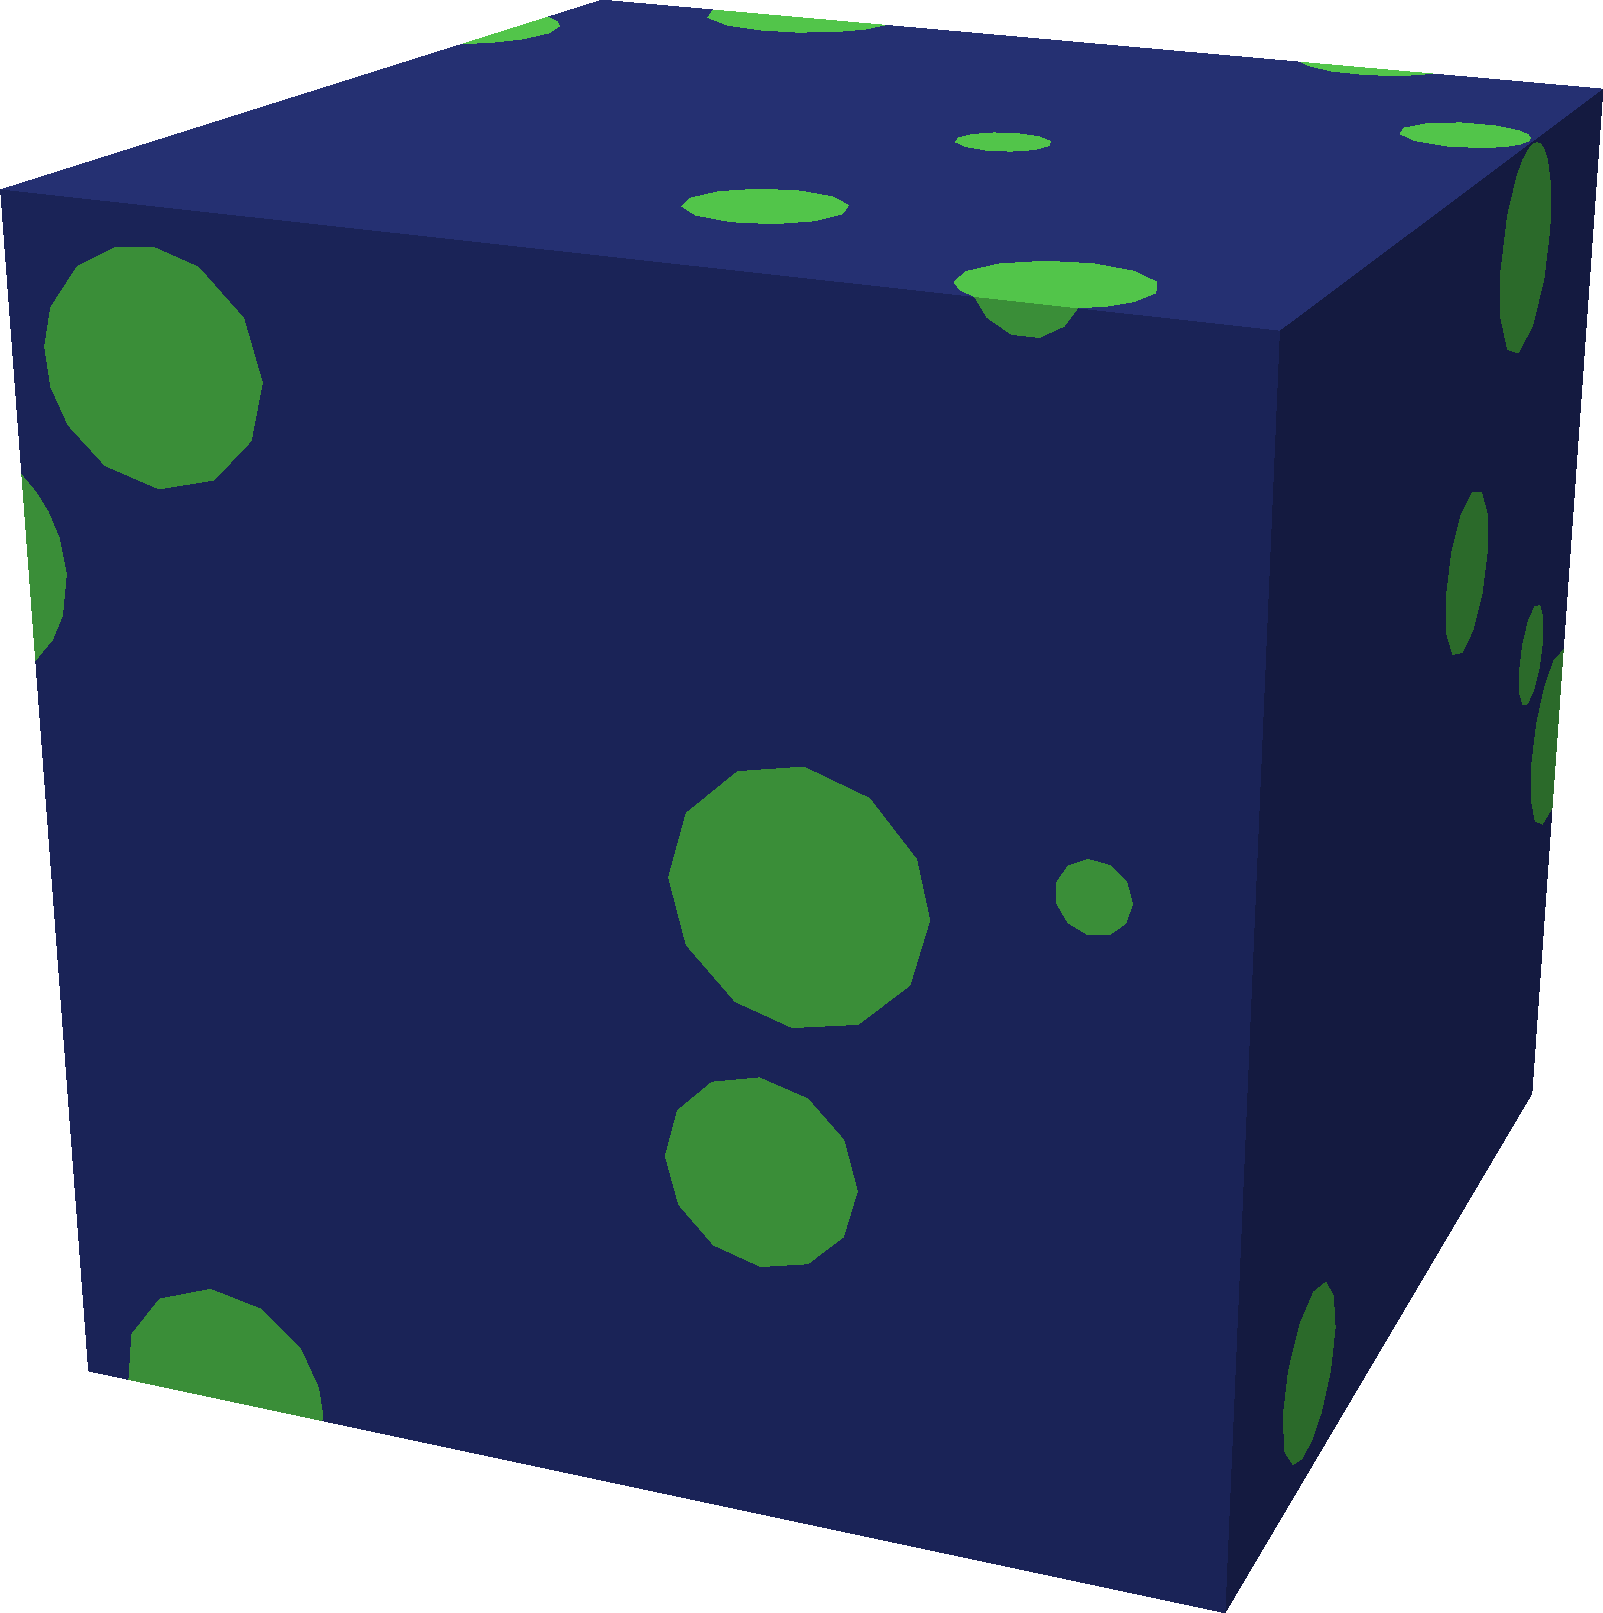
\includegraphics[width=0.4\linewidth]{rve6.png}
 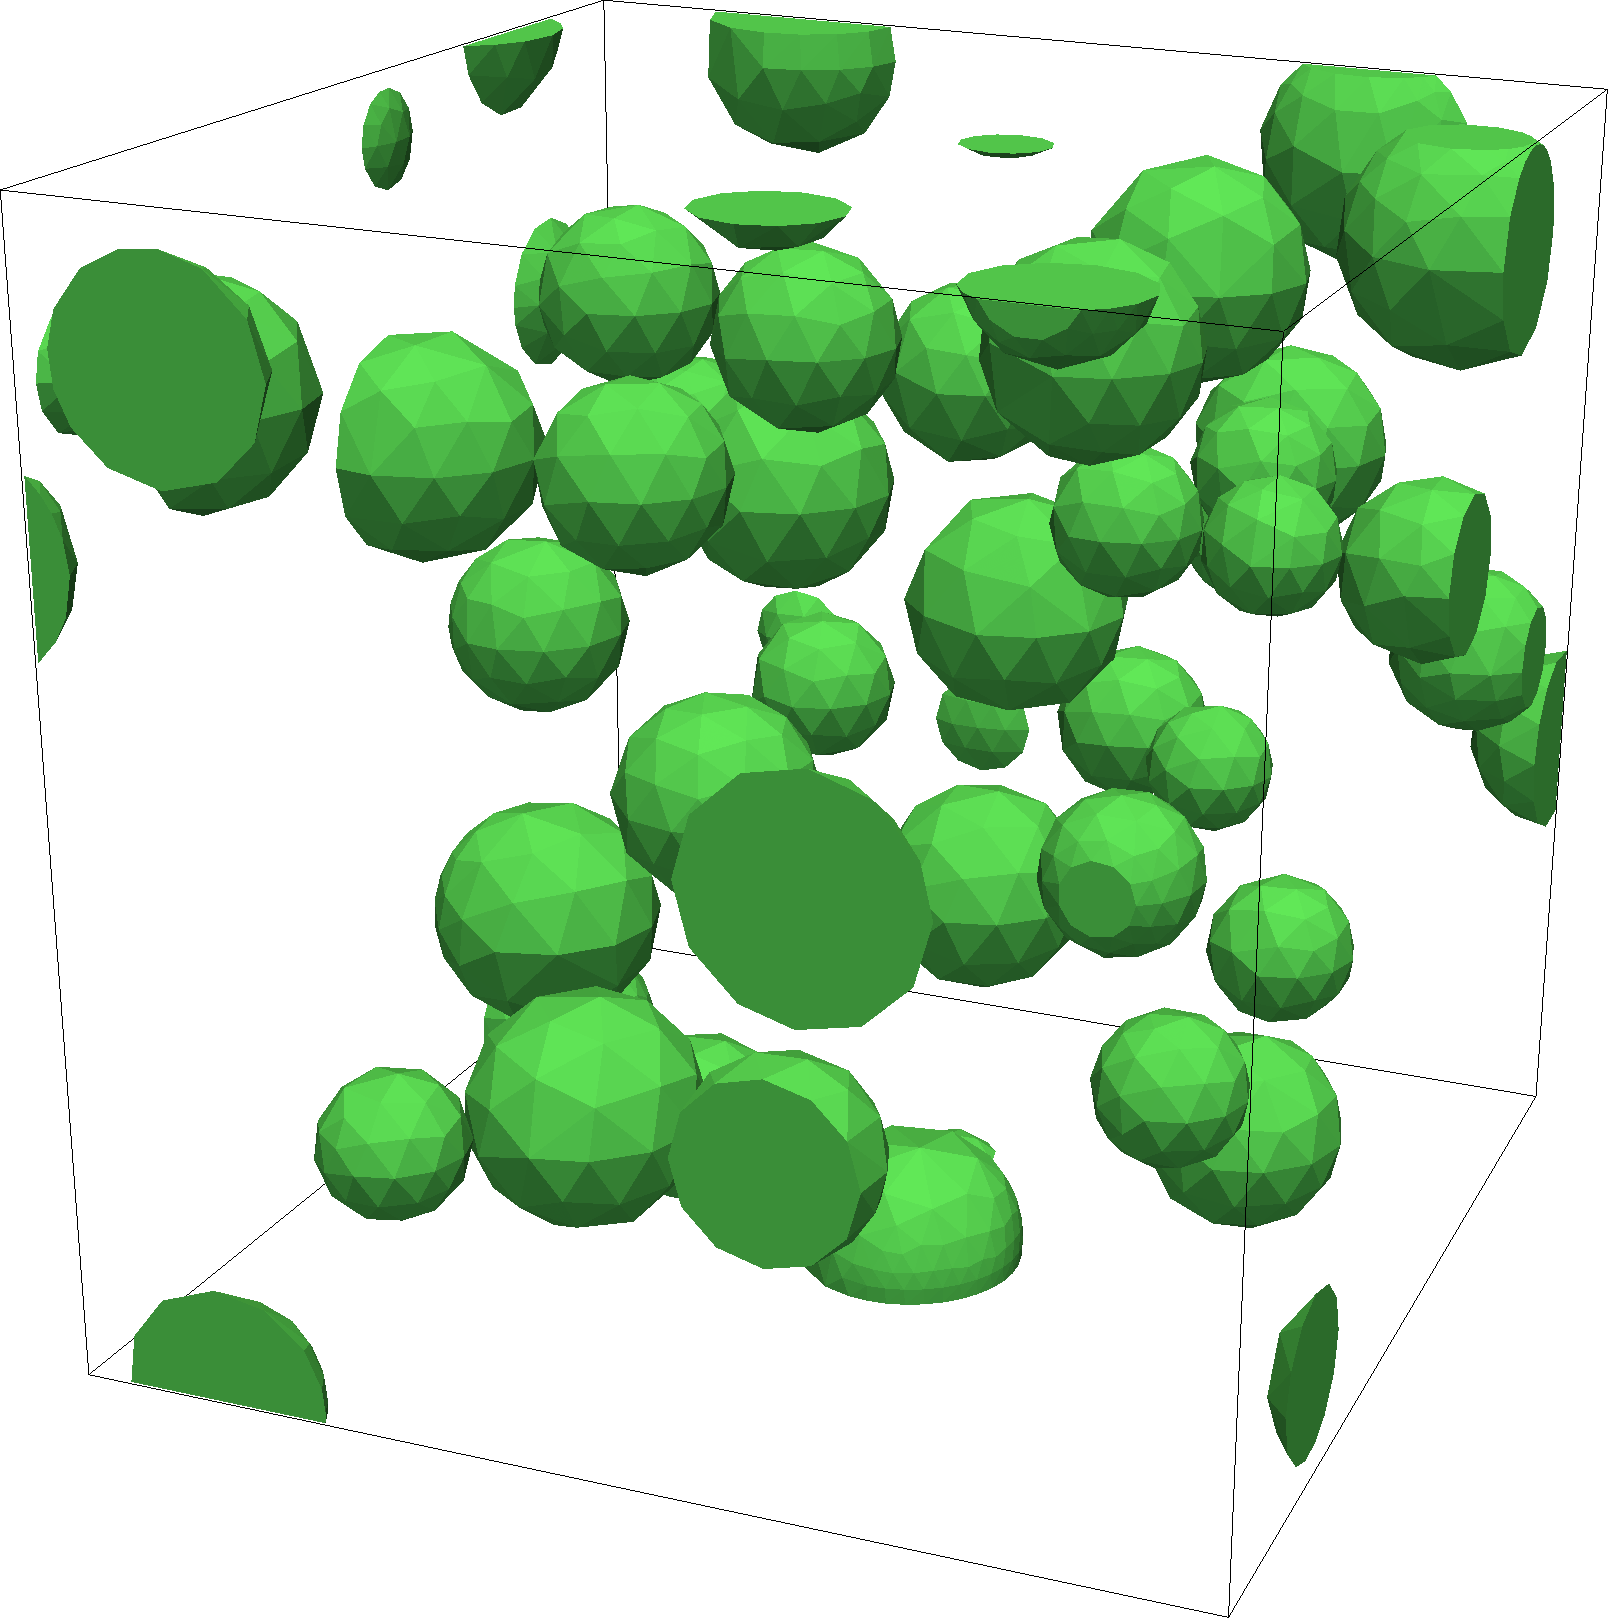
\includegraphics[width=0.4\linewidth]{rve6_inc.png}
\caption{SVE-cube with sample realization of particle composite of size $6\times 6\times 6$}
\label{fig:rve_sample6}
\end{figure}

\begin{figure}[H]
\centering
 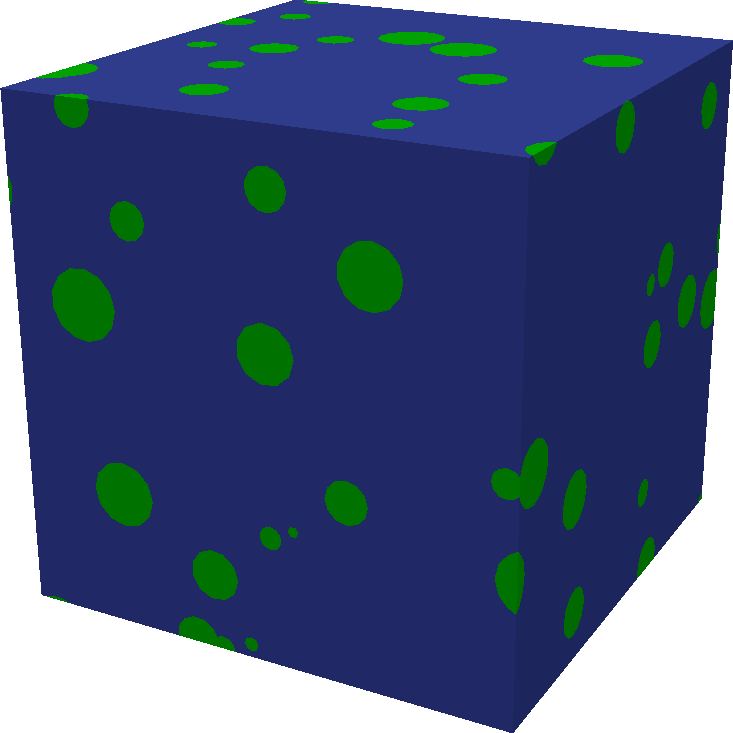
\includegraphics[width=0.4\linewidth]{rve9.png}
 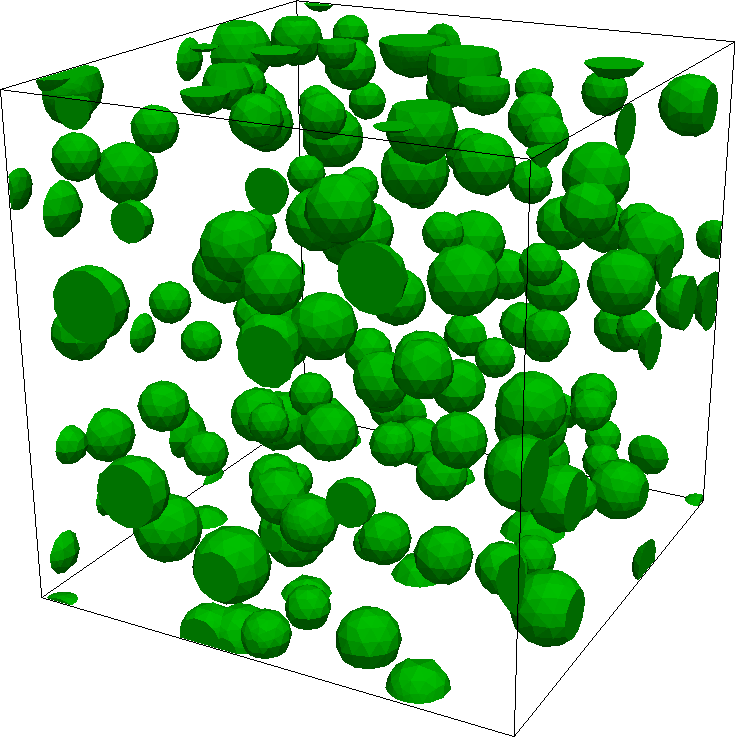
\includegraphics[width=0.4\linewidth]{rve9_inc.png}
\caption{SVE-cube with sample realization of particle composite of size $9\times 9\times 9$}
\label{fig:rve_sample9}
\end{figure}

Now, for sufficiently large size of the SVE (for any given realization of a random composite), we may assume that the macroscale response is isotropic corresponding to the effective moduli $\bar{G}$ and $\bar{C}$ ($=\bar{K}^{-1}$).
However, even for a smaller SVE-size, it is possible to compute an ``apparent'' value of $\bar{G}$ by the minimization
\begin{align}
 \min \frac12 \sum_{ijkl} (\bar{\tf E} - 2 \bar{G} \tf I_\dev)_{ijkl}^2 \implies \bar{G} = \frac12 \frac{\sum_{ijkl}(\tf I_\dev)_{ijkl}(\bar{\tf E})_{ijkl}}{\sum_{ijkl} (\tf I_\dev)_{ijkl}^2}
\end{align}
where $\tf I_\dev$ is the deviatoric fourth order identity tensor such that the isotropic part of $\bar{\tf E}$ can be expressed as $\bar{\tf E}_{\mathrm{iso}} = 2 \bar{G} \tf I_\dev$ in standard fashion.

For the finite element analysis of the SVE-problems, tetrahedral elements with socalled Mini-element approximations are utilized.
This type of element is defined by linear approximation plus a bubble function for $\ta u$ and linear approximation for $p$, cf.\ \cite{arnold_stable_1984}.

The RVE-problems with the different boundary conditions are implemented in the open source C++ code OOFEM (\texttt{www.oofem.org}) \cite{patzak_design_2001} and are available under the name \texttt{Mixed\-Gradient\-Pressure}.
However, due to the difficulty of constructing $\set{T}_\rve$, the present implementation of the weakly periodic boundary conditions is based on global polynomials for discretizing $\set{T}_\rve$.
Thus, only a lower bound for the true periodicity is obtained.
Due to the high computational cost, only the Neumann and Dirichlet boundary conditions are used in the numerical examples in this paper.


\subsection{Homogenization of macroscopically incompressible response --- A convergence study}
The first series of SVE-computations were carried out for macroscopically incompressible response, which is obtained when both matrix and particles are completely incompressible.
Taking the shear modulus for the matrix, $G_\mathrm{mat}$, as the reference modulus, we choose $G_\mathrm{part} = 5\,G_\mathrm{mat}$, whereas $C_\mathrm{mat} = C_\mathrm{part} = 0$.
Convergence results for the two extremes of Dirichlet and Neumann boundary conditions are shown in \figref{fig:SVE_comp}.
The mean value and variance of the homogenized shear modulus $\bar{G}$ are shown for increasing SVE-size, represented by $L_\rve$.
Here, a certain number of realizations are used for each value of $L_\rve$, starting with 200 realizations for the smallest SVE size ($L_\rve = 1$) and ending up with only 4 realizations for the largest SVE-size ($L_\rve$).
The larger SVE:s do not need as many realizations, which is verified by the small variance as can be seen in \figref{fig:SVE_comp}.
An RVE is obtained when the variance goes to zero, and the mean value converges, which is the case when the SVE-size is sufficiently large.
In the present case, for engineering purposes, we consider $L_\rve=9$ sufficiently large to qualify as an RVE.

\begin{figure}[htbp!]
\centering
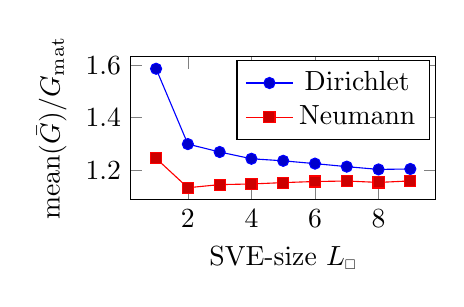
\begin{tikzpicture}
  \begin{axis}[ width=0.45\linewidth, height=0.28\linewidth, xlabel=SVE-size $L_\rve$, ylabel=$\mathop{\mathrm{mean}}(\bar{G})/G_\mathrm{mat}$]
  \addplot table[color=blue,x=size,y=d_mean] {
size d_mean d_var
1.000000   1.586624   0.489829
2.000000   1.299371   0.029517
3.000000   1.269267   0.007279
4.000000   1.243507   0.002562
5.000000   1.235669   0.000874
6.000000   1.224925   0.000534
7.000000   1.213449   0.000258
8.000000   1.202848   0.000205
9.000000   1.204560   0.000033
  };
 \addlegendentry{Dirichlet}
  \addplot table[color=red,x=size,y=n_mean] {
size n_mean n_var
1.000000   1.245017   0.110729
2.000000   1.133016   0.006438
3.000000   1.144928   0.002252
4.000000   1.147371   0.001132
5.000000   1.152570   0.000572
6.000000   1.156771   0.000293
7.000000   1.158645   0.000139
8.000000   1.153319   0.000129
9.000000   1.158993   0.000039
  };
\addlegendentry{Neumann}
  \end{axis}
\end{tikzpicture}
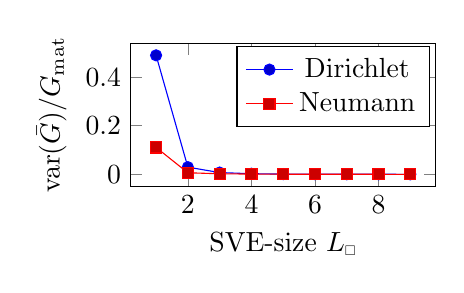
\begin{tikzpicture}
  \begin{axis}[ width=0.45\linewidth, height=0.28\linewidth, xlabel=SVE-size $L_\rve$, ylabel=$\mathop{\mathrm{var}}(\bar{G})/G_\mathrm{mat}$]
  \addplot table[color=blue,x=size,y=d_var] {
size d_mean d_var
1.000000   1.586624   0.489829
2.000000   1.299371   0.029517
3.000000   1.269267   0.007279
4.000000   1.243507   0.002562
5.000000   1.235669   0.000874
6.000000   1.224925   0.000534
7.000000   1.213449   0.000258
8.000000   1.202848   0.000205
9.000000   1.204560   0.000033
  };
\addlegendentry{Dirichlet}
  \addplot table[color=red,x=size,y=n_var] {
size n_mean n_var
1.000000   1.245017   0.110729
2.000000   1.133016   0.006438
3.000000   1.144928   0.002252
4.000000   1.147371   0.001132
5.000000   1.152570   0.000572
6.000000   1.156771   0.000293
7.000000   1.158645   0.000139
8.000000   1.153319   0.000129
9.000000   1.158993   0.000039
  };
\addlegendentry{Neumann}
  \end{axis}
\end{tikzpicture}
\caption{Statistical comparison of the influence of the boundary conditions (Dirichlet, Neumann) on the macroscale shear modulus, $\bar{G}$.}
\label{fig:SVE_comp}
\end{figure}




%[ 0.48982921  0.02951732  0.0072791   0.00256187  0.00087397  0.00053358]
%[ 0.1107292   0.00643845  0.00225217  0.00113156  0.00057236  0.00029335]


The deformed shape for a typical sample SVE of size $L_\rve = 6$ with Neumann boundary condition is shown in \figref{fig:def_rve6}.

\begin{figure}[htpb!]
\centering
 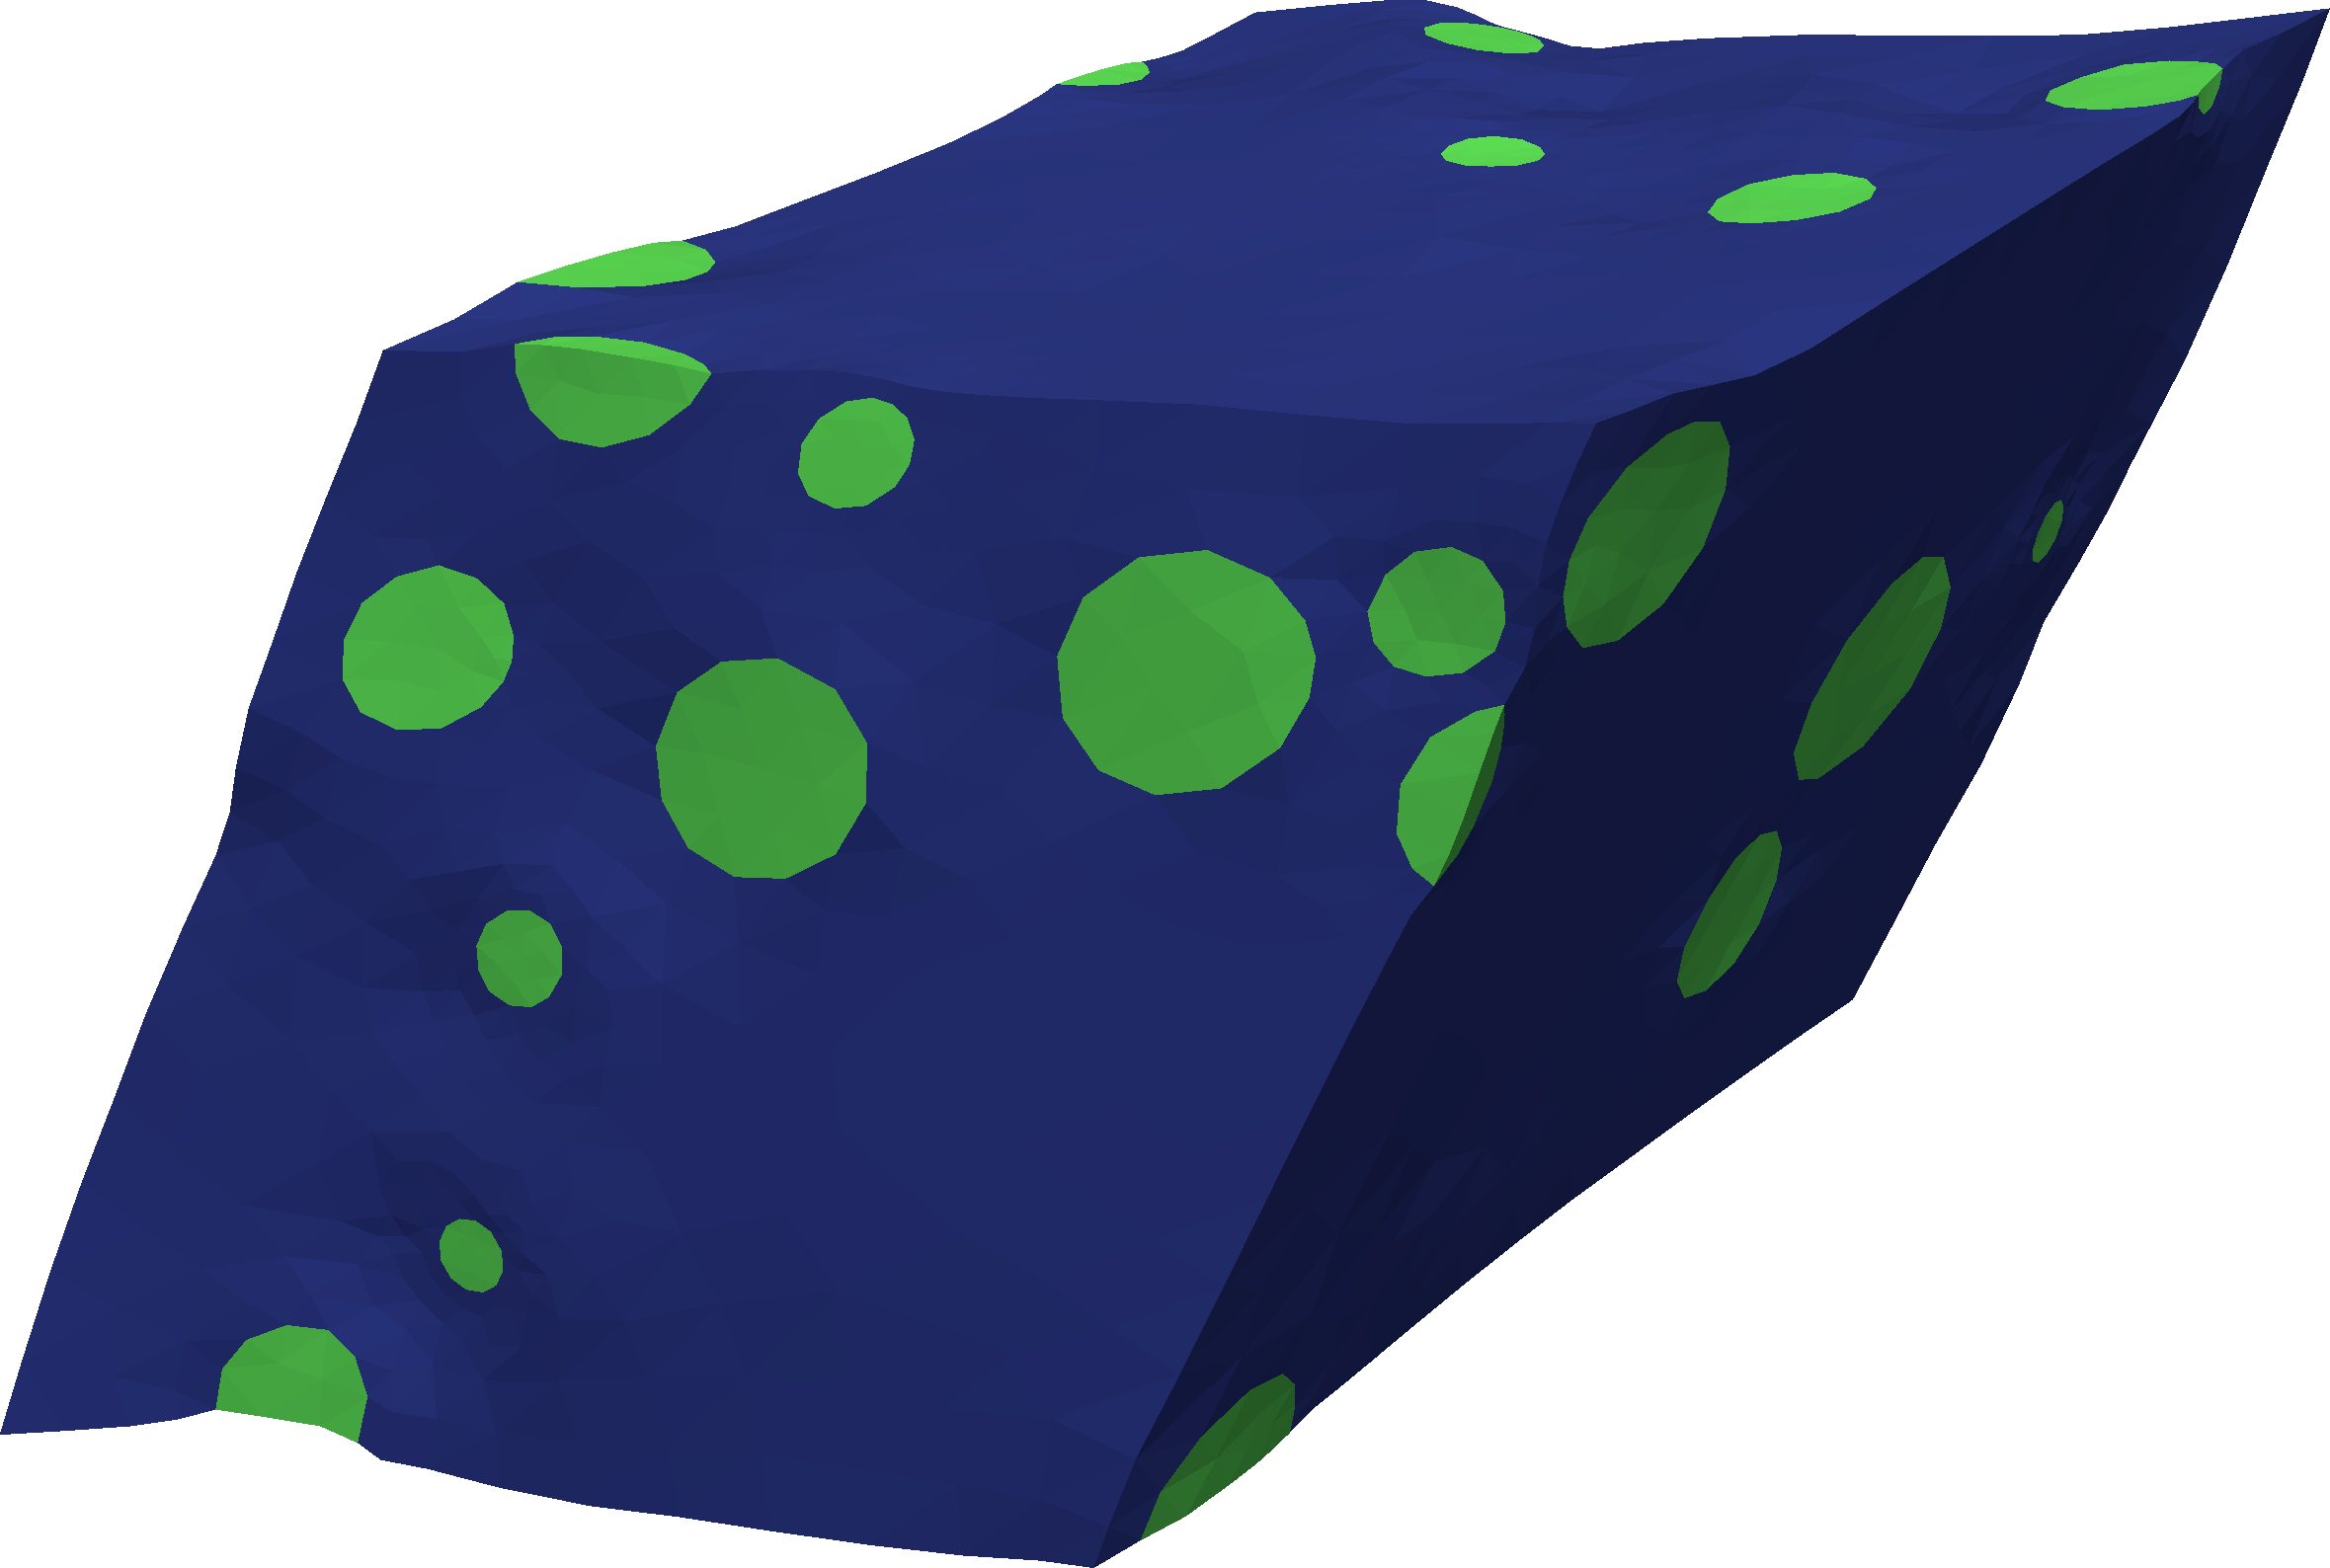
\includegraphics[width=0.5\linewidth]{rve6_def.png}
\caption{A sample SVE subjected to macroscopic pure shear $(\bar{\ts\epsilon}_\dev)_{ij} = 0.4[1 - \delta_{ij}]$.}
\label{fig:def_rve6}
\end{figure}



\subsection{Seamless transition from macroscopically compressible to incompressible response}
In the second series of computations, we show how the homogenization scheme can seamlessly handle the transition from the macroscopically compressible to the incompressible response.
Here, it is assumed that incompressible particles, defined by $G_\mathrm{part} = 5\,G_\mathrm{mat}$ and $C_\mathrm{part} = 0$ (as before), are embedded in a matrix material with $C_\mathrm{mat}\geq 0$.
Only the situation with Dirichlet boundary conditions is considered (without affecting the generality of the main conclusion from the results).
In \figref{fig:RVE_compressibility} it is shown how the homogenized properties are affected by the matrix compliance, $C_\mathrm{mat}$, for a given (fixed) realization and given SVE-size ($L_\rve = 9$, cf. \figref{fig:rve_sample9}),  thus defining an RVE.
Clearly, rather than choosing $C_\mathrm{mat}$ as the variable material property, one may choose Poisson's ratio $\nu_\mathrm{mat}$ via the elementary relation
\begin{align}
 \nu = \frac{3-2\,C\,G}{6 + 2\,C\,G}
\end{align}
which is also used in \figref{fig:RVE_compressibility}.

\begin{figure}[htbp!]
\centering
\begin{tikzpicture}
  \begin{axis}[ width=0.45\linewidth, height=0.28\linewidth,
    x tick label style = {footnotesize},
    xlabel=$C_\mathrm{mat}\times G_\mathrm{mat}$,
    ylabel=$\bar{C}\times G_\mathrm{mat}$,
    extra x ticks={1.09091, 0.75000, 0.46154, 0.21429, 0.00000},
    extra x tick labels={0.1, 0.2, 0.3, 0.4, 0.5}, 
    every extra x tick/.style = {
        xticklabel style = {name=name label},
        xtick pos = right,
        xticklabel pos = right,
        xtick align = outside
    }
    ]
  \addplot table[color=blue,x=M,y=C] {macro_k9.matdata};
  \end{axis}
  \node at (2.1,2.8) { $\nu_\mathrm{mat}$ };
\end{tikzpicture}
\begin{tikzpicture}
  \begin{axis}[ width=0.45\linewidth, height=0.28\linewidth,
    x tick label style = {footnotesize},
    xlabel=$C_\mathrm{mat}\times G_\mathrm{mat}$,
    ylabel=$\bar{G}/G_\mathrm{mat}$,
    extra x ticks={1.09091, 0.75000, 0.46154, 0.21429, 0.00000},
    extra x tick labels={0.1, 0.2, 0.3, 0.4, 0.5}, 
    every extra x tick/.style = {
        xticklabel style = {name=name label},
        xtick pos = right,
        xticklabel pos = right,
        xtick align = outside
    }
    ]
  \addplot table[color=blue,x=M,y=G] {macro_k9.matdata};
  \end{axis}
  \node at (2.1,2.8) { $\nu_\mathrm{mat}$ };
\end{tikzpicture}
\caption{Homogenized results from a single RVE with Dirichlet boundary condition.
Dependence of effective properties $\bar{C}$ and $\bar{G}$ on the bulk compliance $C_\mathrm{mat}$ for fixed values of $G_\mathrm{part} = 5\,G_\mathrm{mat}$ and $C_\mathrm{part} = 0$.}
\label{fig:RVE_compressibility}
\end{figure}

The computational results verify that the homogenization framework is able to handle the transition from macroscale compressibility to incompressibility when $C_\mathrm{mat}\to 0$ in a seamless fashion without any algorithmic changes.
That macroscopical incompressibility is obtained is verified by the computed value $\bar{C} = 0$.
It is also noted in \figref{fig:RVE_compressibility} that the affect on $\bar{G}$ is more pronounced, however quite limited, when incompressibility is approached.

\section{Conclusions and outlook}
In this paper we have introduced a variationally consistent homogenization scheme for heterogeneous solids, whose constituents may be incompressible in the extreme case.
The transition from macroscopically compressible to incompressible states (which is the extreme result when all constituents are incompressible) is handled in a completely seamless fashion.
Based on a mixed formulation on the fine scale, it has been demonstrated how the concept of variationally consistent homogenization can be adopted to derive the pertinent two-scale problem.
The proposed canonical formulation of the problem on an underlying Representative Volume Element (RVE) is an extension of the formulation presented in Öhman et al. (2013), allowing for a general choice of boundary conditions.
Moreover, the canonical formulation has been shown to satisfy the generalized macrohomogeneity condition.
The FE-setting on both scales (macroscale and RVE) is based on the standard $(\ta{u},p)$-formulation, and the Mini-element approximation with a bubble function is adopted for the RVE-problem.
All implementation and numerical results pertain to 3D-cubes.

It was shown that theoretical bounds on the ``homogenized energy density'' for weakly periodic boundary conditions on the RVE are obtained by imposing Dirichlet and Neumann boundary conditions.
The computational results from a statistical analysis verify the convergence of these bounds with increasing SVE-size.
As to the computational cost of solving the RVE-problem with the different types of boundary conditions for the standard compressible problem and the present (in)compressible one, it is concluded that the Neumann boundary condition is quite cost-neutral.
However, applying the Dirichlet boundary condition to the canonical RVE-format means a noticeable additional cost, since the additional (global) variable $\bar{e}$ is required in order to account for the (possibly vanishing) macroscale volumetric deformation.
In this context, we remark that imposing weak periodicity would infer a further increased computational cost associated with the boundary discretization of tractions in $\set{T}_\rve$; hence, it is conjectured that exploiting the standard Dirichlet and Neumann conditions computations and drawing conclusions about their bounding character would be a most competitive approach in FE\textsuperscript{2}-computations.

As to future developments, it is desirable to further exploit the concept of weakly periodic boundary conditions; however, constructing basis functions for $\set{T}_\Box$ in 3D is not a trivial task.
Of course, it is also of interest to compare with the classical condition of strongly periodic fluctuations, which is defined by replacing \cref{eq61b} with
\begin{align}
    \set{U}_\rve^{\Periodic,\fluct} &= \{\ta{v}\in \set{U}_\rve^\fluct \,|\,\, \jmp{\ta{v}}=\ta{0} \text{ on } \Gamma_\rve \}
\end{align}
and performing the corresponding steps up to \cref{eq:weak_form_dirichlet}.
However, this method has the definite drawback that the meshing software must produce strictly periodic meshes.


In a forthcoming paper, the proposed theoretical framework will be applied to the problem of sintering, a characteristic of which is that the microstructure evolves from being highly porous to becoming completely dense.
The ``compaction'' process is driven by surface tension along the particle-pores boundaries until the pore have completely disappeared, cf. Öhman et al. (2013).


% 
% 
% \section{Conclusions and outlook}
% In this paper we have introduced a variationally consistent homogenization scheme for macroscopically incompressible micro structures.
% We have derived a canonical form of the RVE-problem which has the same strong form as the macroscale problem, while still satisfying the macrohomogeneity condition.
% This allows for straight forward finite element implementations, as both scales use the same standard $(\ta u,p)$-formulation.
% 
% We have also shown the bounds for the periodic boundary condition on an RVE by deriving the Dirichlet and Neumann boundary conditions.
% The proposed method is required whenever an RVE exhibit near or complete incompressibility, and works seamlessly if an RVE transitions from compressible to incompressible response.
% 
% 
% The computational cost of the Neumann boundary condition is equivalent to that of the classical (compressible) Neumann boundary condition.
% The Dirichlet boundary condition requires a global unknown to relax the macroscopic volumetric deformation, which has a significant computational cost compared to the classical (compressible) Dirichlet boundary condition.
% The weakly periodic boundary condition has a has a large computational cost (depending heavily on the choice of discretization of $\set T_\rve$), so the bounds given by the Dirichlet and Neumann boundary condition is likely to be the most efficient solution for FE\textsuperscript{2} simulations.
% 
% 
% Due to the difficult procedure of constructing basis functions for $\set T_\rve$ for 3D geometries, the current implementation relies on global polynomials where the computational cost drastically increases with the order of the polynomials, while only showing a marginal improvement compared to the Neumann boundary condition.


%\clearpage
%\printbibliography

%\bibliography{Multiscale,Sintering,FEM_Software,Mesh}
%\bibliographystyle{plain}

%\bibliographystyle{elsarticle-num}
%\bibliography{ref_sintering}
%\bibliography{ref_multiscale}

\appendix
\setcounter{equation}{0}
\renewcommand{\theequation}{A-\arabic{equation}}

\section{Appendix}

\subsection{Variationally Consistent Homogenization (VCH)}
\label{appendix:1}

\subsubsection{VMS-approach -- Scale separation and homogenization}

Classical model-based homogenization can be formulated in the spirit of the Variational MultiScale method (VMS), cf.\ \cite{hughes_variational_1998}, \cite{larson_adaptive_2007}.
We introduce the abbreviated notation $z = (\ta u, p) \in \set{Z} = \set U \times \set P$, where $\set Z$ represents the space of fine-scale (non-homogenized) solutions to the system \cref{eq2},
which may conveniently be abbreviated in abstract form as the residual equation\footnote{Henceforth in this Appendix, we consider the abstract formulation of a multifield problem based on a given set of balance (or constraint) equations.
No explicit reference to the specific character of the underlying problem is made.}
%-------------------------------------------------------------------------------------------------------------------------------
\begin{align}
 R(z; \delta z) \defeq R_\Omega(z; \delta z) + R_\Gamma(z;\delta z) = 0\quad \forall\;\delta z\in \set Z^0
\label{eq:A1}
\end{align}
%-------------------------------------------------------------------------------------------------------------------------------
where $\set Z^0 = \set U^0 \times \set P$ is the test space and where each $\ta u\in \set U^0$ vanishes on the Dirichlet part of $\Gamma$.

A multiscale formulation of \cref{eq:A1} is defined by the hierarchical split $\set Z = \set Z^\macro \oplus \set Z^\fluct$, where $\set Z^\macro$ contains smooth macroscale functions and $\set Z^\fluct$ is the hierarchical complement of $\set Z^\macro$ that, typically, represents the fine-scale features.
It is assumed that each $z\in \set Z$ can be split uniquely as $z = z^\macro + z^\fluct$ such that $z^\macro \in \set Z^\macro$ and $z^\fluct \in \set Z^\fluct$.
Therefore, solve $z^\macro \in \set Z^\macro$, $z^\fluct \in \set Z^\fluct$ such that \cref{eq:A1} can be represented by the set of equations
%------------------------------------------------------------------------------------------------------------------------------------------------
\begin{subequations}\label{eq:A2}
\begin{alignat}{3}
\label{eq:A2a} & R(z^\macro + z^\fluct; \delta z^\macro) &&= 0 \quad &&\forall\;\delta z^\macro \in \set Z^{\macro,0}\\
\label{eq:A2b} & R(z^\macro + z^\fluct; \delta z^\fluct) &&= 0       &&\forall\;\delta z^\fluct \in \set Z^{\fluct}
\end{alignat}
\end{subequations}
%-----------------------------------------------------------------------------------------------------------------------------
Without introducing further assumptions (approximations), the dimension of the original problem has not changed, i.e.\ \cref{eq:A2} represent two global problems whose solution requires the same computational effort as does \cref{eq:A1}.
In order to reduce the problem dimension based on homogenization (via the assumption of scale separation), we introduce the following key assumptions:

\begin{itemize}
\item The integrands in the pertinent volume integrals are replaced by a running volume average on RVE's of the type introduced in \cref{eq16ba}
such that, typically, the residual in \cref{eq:A2a} can be rewritten in terms of the contributions defined on each RVE as
%--------------------------------------------------------------------------------------------------------------------------
\begin{align}
\label{eq:A106} R_\Omega(z;\delta z) = \int_\Omega R_\rve(z;\delta z)(\bar{\ta x})\dif\Omega
\end{align}
%------------------------------------------------------------------------------------------------------------------------------
where $R_\rve$ is the RVE-residual that is localized to the Representative Volume Element (RVE).
In practice (in FE-analysis), quadrature is used such that the evaluation of $R_\rve$ is carried out only in the Gauss points.

Furthermore, for the sake of simplicity we assume smoothness of boundary terms, such that $R_\Gamma(z; \delta z^\macro) \approx R_\Gamma(z^\macro;\delta z^\macro)$, i.e.\ no boundary homogenization is necessary.

\item Local approximations for the fluctuation field $z^\fluct$ are introduced in the spirit of VMS.
This means that $z^\fluct \approx \tilde{z}^\fluct\{z^\macro\}\in\set{Z}_\rve^{\fluct}$ is the \emph{approximate} solution\footnote{Curly brackets $\{\bullet\}$ indicate implicit function.} of the fine-scale 
equation \cref{eq:A2b} for given $z^\macro$, i.e.\ \cref{eq:A2b} is replaced by ``closed'' RVE-problems (in the macroscale quadrature points) associated with a particular choice of boundary conditions on $\Omega_\rve$.
In this paper we obtain such ``closed'' RVE-problems by choosing  weakly periodic boundary conditions.
\end{itemize}
Returning to \cref{eq:A2a}, we now replace this problem by the approximate, homogenized, problem
%---------------------------------------------------------------------------------------------------------------------------------------------
\begin{multline}
\label{eq:A3} R(z^\macro+\tilde{z}^\fluct\{z^\macro\};\delta z^\macro) = \int_\Omega R_\rve(z^\macro+\tilde{z}^\fluct\{z^\macro\};\delta z^\macro)(\bar{\ta x})\dif\Omega
 \\
 + R_\Gamma(z^\macro, \delta z^\macro) = 0 \quad \forall\;\delta z^\macro \in \set Z^{\macro,0}
\end{multline}
%--------------------------------------------------------------------------------------------------------------------------------
which has the same dimension as \cref{eq:A2a}.
We note that \cref{eq:A3} represents a valid homogenization problem for any given choice of $\set{Z}_\rve^{\fluct}$; however, to preserve typical Galerkin properties, such as symmetry of the macroscale tangent operator when such symmetry is inherent in the underlying fine-scale problem, it is crucial to satisfy the VCMC.

\subsubsection{Variationally Consistent Macrohomogeneity Condition (VCMC)}

We shall assume that there exists a potential $\Pi(z)$ such that \cref{eq:A3} represents the stationary point of $\Pi(z)$, i.e.\ it is assumed that
%---------------------------------------------------------------------------------------------------------------------------------------
\begin{align}
\label{eq:A4} R(z;\delta z) = \Pi'(z;\delta z) \defeq \frac{\dif}{\dif\epsilon}\Pi(z+\epsilon\delta z)|_{\epsilon = 0} = 0\quad \forall\;\delta z \in \set Z^0
\end{align}
%------------------------------------------------------------------------------------------------------
Next, we introduce the crucial \emph{approximation} (restriction) $z \approx z^\macro + \tilde{z}^\fluct\{z^\macro\}$ before evaluation of the stationarity conditions, whereby we obtain
%---------------------------------------------------------------------------------------------------------------------------------------
\begin{align}
\label{eq:A5} \Pi_{z^\macro}'\{z^\macro;\delta z^\macro\} & \defeq
\frac{\dif}{\dif\epsilon}\Pi(z^\macro+\epsilon \delta z^\macro+\tilde{z}^\fluct\{z^\macro+\epsilon \delta z^\macro\})|_{\epsilon = 0} \nonumber \\
& =
R(z^\macro + \tilde{z}^\fluct\{z^\macro\}; \delta z^\macro + (\tilde{z}^\fluct)'\{z^\macro;\delta z^\macro\}) = 0\quad \forall\;\delta z^\macro\in\set Z^{\macro,0}
\end{align}
%------------------------------------------------------------------------------------------------------------------------------------------
where $(\tilde{z}^\fluct)'\{z^\macro;\delta z^\macro\}$ denotes the sensitivity (or directional derivative) of $\tilde z^\fluct$ for a variation $\delta z^\macro$ of the macroscale solution $z^\macro$.
Hence, the choice of test function in \cref{eq:A5} is restricted as compared to \cref{eq:A4}, and this restriction represents a ``generalized Galerkin property'' in terms of the underlying macroscale functions in $\set Z^\macro$.
Moreover, and most importantly, \cref{eq:A5} is completely equivalent to the homogenized problem \cref{eq:A3} if it is possible, for any given $z^\macro\in\set Z^{\macro}$, to satisfy the constraint
%---------------------------------------------------------------------------------------------------------------------------------------------
\begin{align}
\label{eq:A6a} R(z^\macro + \tilde z^\fluct\{z^\macro\}; (\tilde{z}^\fluct)'\{z^\macro;\dif z^\macro\}) = 0\quad \forall\;\dif z^\macro\in\set Z^{\macro,0}(z^\macro)
\end{align}
%-------------------------------------------------------------------------------------------------------------------------------------------------
or, equivalently,
%---------------------------------------------------------------------------------------------------------------------------------------------
\begin{align}
\label{eq:A6b} R(z^\macro + \tilde z^\fluct\{z^\macro\}; \dif\tilde{z}^\fluct) = 0\quad \forall\;\dif\tilde{z}^\fluct\in\tilde{\set Z}'^{\fluct}(z^\macro)
\end{align}
%-------------------------------------------------------------------------------------------------------------------------------------------------
where the test space $\tilde{\set Z}'^{\fluct}(z^\macro)$, which is the tangent space to the approximation space, is defined as
%----------------------------------------------------------------------------------------------------------------
\begin{align}
    \tilde{\set{Z}}'^{\fluct}(z^\macro)\defeq\{\set{Z}^\fluct\ni \dif z^\fluct = (\tilde{z}^\fluct)'\{z^\macro;\dif z^\macro\},\,
    \dif z^\macro\in \set{Z}^{\macro,0}\}
\label{eq:A6c}
\end{align}
%----------------------------------------------------------------------------------------------------------------------
Hence, any $\dif \tilde{z}^\fluct\in\tilde{\set{Z}}'^{\fluct}(z^\macro)$ is a sensitivity of the fluctuation field $\tilde{z}^\fluct$ for a differential change of the macroscale field $z^\macro$ within the considered RVE.
It is computed from the tangent problem that is associated with the RVE-problem.
We refer to \cref{eq:A6a} or \cref{eq:A6b} as a ``Variationally Consistent (generalized) Macrohomogeneity Condition'' (VCMC).
Obviously, a sufficient condition for these identities to hold true is to require the RVE-residual to vanish on each RVE (in each quadrature point), i.e.\ to ensure that
%--------------------------------------------------------------------------------------------------------------------------------------
\begin{align}
\label{eq:A8} R_\rve(z^\macro + \tilde z^\fluct\{z^\macro\};(\tilde{z}^\fluct)'\{z^\macro;\delta z^\macro\}) = 0\quad \forall\;z^\macro,\delta z^\macro\in\set Z^{\macro}|_{\Omega_\rve}\times\set Z^{\macro,0}|_{\Omega_\rve}
\end{align}
%----------------------------------------------------------------------------------------------------------------------------------------------
An even stronger condition is to require that $R_\rve(z;\delta z^\fluct) = 0$ for \emph{any} $\delta z^\fluct$ in a given set of functions that is defined locally for the considered RVE without requiring any implicit (or explicit) 
coupling to the sensitivity field $(\tilde{z}^\fluct)'\{z^\macro;\delta z^\macro\}$, which obviously defines a restricted choice of test functions.
In such a case, the VCMC can be identified as precisely the classical Hill-Mandel macrohomogeneity condition.

Finally, we remark that the VCMC ensures that the macroscale tangent operator becomes symmetrical, since it holds that
%---------------------------------------------------------------------------------------------------------------------------------------
\begin{align}
\label{eq:A9} R'(z;\delta z_1,\delta z_2) = \Pi''(z;\delta z_1,\delta z_2) \defeq \frac{\dif}{\dif\epsilon}\Pi'(z+\epsilon\delta z_2;\delta z_1)|_{\epsilon=0}\quad \forall\;\delta z_1,\delta z_2 \in \set Z^0
\end{align}
%------------------------------------------------------------------------------------------------------
With the introduced approximation $z^\fluct \approx \tilde{z}^\fluct\{z^\macro\}$, the test functions in \cref{eq:A9} are chosen as
%---------------------------------------------------------------------------------------------------------------------------------------
\begin{align}
\label{eq:A10} \delta z_i \approx \delta z_i^\macro + (\tilde{z}^\fluct)'\{z^\macro;\delta z_i^\macro\} \quad \forall\;\delta z_i^\macro\in\set Z^{\macro,0}, \,\, i=1,2
\end{align}
%------------------------------------------------------------------------------------------------------------------------------------------



\subsection{Homogenized macroscale energy}
\label{appendix:macroEnergy}

In order to show that $\bar{\psi}_\rve\{\bar{\ts\epsilon}_\dev, \bar{p}\}$ serves as the ``macroscale energy density'' for $\bar{\ts\sigma}_\dev$ and $\bar{e}$, expressed by the relations \cref{eq88}, we first recall the identity
\begin{align}
 \bar{\psi}_\rve\{\bar{\ts\epsilon}_\dev, \bar{p}\} = \Pi_\rve(\bar{\ts\epsilon}_\dev, \bar{p}; \ta u\epspargs, p\epspargs, \ta t\epspargs, \bar{e}\epspargs)
\end{align}
where the RVE-potential $\Pi_\rve$ was defined in \cref{eq81}.
Working out the total differential w.r.t.\ $\bar{\ts\epsilon}_\dev$ and $\bar{p}$ at equilibrium, we obtain
\begin{align}
 \dif\bar{\psi}_\rve\epspargs = 
  &\Pi_\rve(\dif\bar{\ts\epsilon}_\dev, \bar{p}; \ta u\epspargs, p\epspargs, \ta t\epspargs, \bar{e}\epspargs) +
\nonumber\\
  &\Pi_\rve(\bar{\ts\epsilon}_\dev, \dif\bar{p}; \ta u\epspargs, p\epspargs, \ta t\epspargs, \bar{e}\epspargs) +
\nonumber\\
  &(\Pi_\rve)'_u(\bar{\ts\epsilon}_\dev, \bar{p}; \ta u\epspargs, p\epspargs, \ta t\epspargs, \bar{e}\epspargs; \dif\ta u) +
\nonumber\\
  &(\Pi_\rve)'_p(\bar{\ts\epsilon}_\dev, \bar{p}; \ta u\epspargs, p\epspargs, \ta t\epspargs, \bar{e}\epspargs; \dif p) +
\nonumber\\
  &(\Pi_\rve)'_t(\bar{\ts\epsilon}_\dev, \bar{p}; \ta u\epspargs, p\epspargs, \ta t\epspargs, \bar{e}\epspargs; \dif\ta t) +
\nonumber\\
  &(\Pi_\rve)'_{\bar{e}}(\bar{\ts\epsilon}_\dev, \bar{p}; \ta u\epspargs, p\epspargs, \ta t\epspargs, \bar{e}\epspargs; \dif\bar{e})
\label{eq:macro_potential_dif}
\end{align}
where we introduced the sensitivities w.r.t.\ changes in $\bar{\ts\epsilon}_\dev$ and $\bar{p}$ as follows:
\begin{align}
 \dif\ta u   &=   (\ta u)'\{\bar{\ts\epsilon}_\dev, \bar{p}; \dif\bar{\ts\epsilon}_\dev, \dif\bar{p}\} \in \set{U}_\rve
\\
 \dif p      &=       (p)'\{\bar{\ts\epsilon}_\dev, \bar{p}; \dif\bar{\ts\epsilon}_\dev, \dif\bar{p}\} \in \set{P}_\rve
\\
 \dif\ta t   &=   (\ta t)'\{\bar{\ts\epsilon}_\dev, \bar{p}; \dif\bar{\ts\epsilon}_\dev, \dif\bar{p}\} \in \set{T}_\rve
\\
 \dif\bar{e} &= (\bar{e})'\{\bar{\ts\epsilon}_\dev, \bar{p}; \dif\bar{\ts\epsilon}_\dev, \dif\bar{p}\} \in \set{R}
\end{align}
Combining these with the \cref{eq:rveStat}, we can see that the last four terms in \cref{eq:macro_potential_dif} vanish, i.e.\ $(\Pi_\rve)'_\bullet(\ldots; \dif\bullet) = 0$.
What remains of the total differential is thus
\begin{align}
 \dif\bar{\psi}_\rve\epspargs = 
  d_\rve(\ta t\epspargs, -\dif\bar{\ts\epsilon}_\dev\cdot[\ta x-\bar{\ta x}]) + \dif\bar{p}\, \bar{e}\epspargs
\label{eq:macro_potential_dif_simple}
\end{align}
Now, we may use \cref{eq:rveStata} and choose $\delta\ta u = \dif\bar{\ts\epsilon}\cdot[\ta x - \bar{\ta x}]$ to obtain
\begin{align}
 -d_\rve(\ta t\epspargs, \dif\bar{\ts\epsilon}_\dev\cdot[\ta x - \bar{\ta x}]) &= 
\nonumber\\
  a_\rve(\ta u\epspargs, \dif\bar{\ts\epsilon}_\dev\cdot[\ta x &- \bar{\ta x}]) + b_\rve(p\epspargs, \dif\bar{\ts\epsilon}_\dev\cdot[\ta x - \bar{\ta x}]) 
\nonumber\\
  &= \homgen{\ts\sigma_\dev}\dprod\dif\bar{\ts\epsilon}_\dev + \homgen{p }\,\underbrace{\dif\bar{\ts\epsilon}_\dev\dprod \ts I}_{=0}
\nonumber\\
  &= \bar{\ts\sigma}_\dev\epspargs \dprod\dif\bar{\ts\epsilon}_\dev
\end{align}
Finally, combining this result with \cref{eq:macro_potential_dif_simple}, we obtain
\begin{align}
 \dif\bar{\psi}_\rve\epspargs = \bar{\ts\sigma}_\dev\epspargs\dprod \dif\bar{\ts\epsilon}_\dev + \bar{e}\epspargs\,\dif\bar{p}
\end{align}
which proves \cref{eq88}.

\subsection{Sensitivity problem}
\label{appendix:sensitivity}

\subsubsection{Dirichlet boundary condition}
Using the perturbations $\bar{\ts\epsilon}_{\dev} + \dif\bar{\ts\epsilon}_{\dev}$ and $\bar{p} + \dif\bar{p}$ in the linearized form of \cref{eq:weak_form_dirichlet} at equilibrium we obtain
\begin{subequations}
\begin{alignat}{2}
    (a_\rve)'(\ta u;\delta\ta{u}^\fluct, \dif \bar{\ts\epsilon}_\dev\cdot[\ta x - \bar{\ta x}] + \dif\ta{u}^\fluct) + b_\rve(\dif p, \delta\ta{u}^\fluct) &= 0
    && \forall \delta\ta{u}^\fluct \in \set{U}_\rve^{\Dirichlet,\fluct}
\\
    b_\rve(\delta p,\dif\ta{u}^\fluct + \dif\bar{e}\,\ta{x}_\mean) + (c^*_\rve)'(p;\delta p,\dif p) &= 0
    && \forall \delta p \in \set{P}_\rve
\\
    b_\rve(\dif p,\delta\bar{e}\,\ta{x}_\mean) &=
    - \dif\bar{p}\,\delta\bar{e}
    && \forall \delta\bar{e} \in \set{R}
\end{alignat}
\end{subequations}
which must hold for any given $\dif\bar{\ts\epsilon}_\dev$ and $\dif\bar{p}$.
We thus consider the cases:
\begin{itemize}
 \item $\dif\bar{\ts\epsilon}_\dev = \ts G_k$ while $\dif\bar{p} = 0$ (with $\ta u^{\macro(k)}_\dev \defeq \ts G_k \cdot[\ta x - \bar{\ta x}]$): For $k = 1, \ldots, 8$, solve for the sensitivities $\ta u_\ded^{\fluct(k)}$, $p_\ded^{(k)}$, $\bar{e}_{\ded}^{(k)}$ from the system 
\end{itemize}
\begin{subequations}\label{eq:d_sensitivities_d}
\begin{alignat}{2}
    (a_\rve)'(\ta{u};\delta\ta{u}^\fluct, \ta u_\ded^{\fluct(k)}) + b_\rve(p_\ded^{(k)},\delta\ta{u}^\fluct) = -(a_\rve)'(\ta{u}&;\delta\ta{u}^\fluct, \ta{u}^{\macro(k)}_\dev)
    &\;& \forall \delta\ta{u}^\fluct \in \set{U}_\rve^{\Dirichlet,\fluct}
\\
    b_\rve(\delta p,\ta u_\ded^{\fluct(k)} + \bar{e}_{\ded}^{(k)}\,\ta{x}_\mean) + (c^*_\rve)'(p;\delta p,p_\ded^{(k)}) &= 0
    &\;& \forall \delta p \in \set{P}_\rve
\\
    b_\rve(p_\ded^{(k)},\delta\bar{e}\,\ta{x}_\mean) &= 0
    &\;& \forall \delta\bar{e} \in \set{R}
\end{alignat}
\end{subequations}

\begin{itemize}
\item $\dif\bar{p} = 1$ while $\dif\bar{\ts\epsilon}_\dev = \ts 0$: Solve for the sensitivities $\ta u_\dep^\fluct$, $p_\dep$, $\bar{e}_{\dep}$ from the system 
\end{itemize}
\begin{subequations}\label{eq:d_sensitivities_p}
\begin{alignat}{2}
    (a_\rve)'(\ta{u};\delta\ta{u}^\fluct, \ta u_\dep^\fluct) + b_\rve(p_\dep,\delta\ta{u}^\fluct) &= 0
    && \forall \delta\ta{u}^\fluct \in \set{U}_\rve^{\Dirichlet,\fluct}
\\
    b_\rve(\delta p,\ta u_\dep^\fluct) + b_\rve(\delta p,\bar{e}_{\dep}\,\ta{x}_\mean) + (c^*_\rve)'(p;\delta p,p_\dep) &= 0
    && \forall \delta p \in \set{P}_\rve
\\
    b_\rve(p_\dep,\delta\bar{e}\,\ta{x}_\mean) &= - \delta\bar{e}
    && \forall \delta\bar{e} \in \set{R}
\end{alignat}
\end{subequations}

Upon using the identity $\bar{\ts\sigma}=\frac{1}{\volume} \int_{\Gamma_\Box} \ts t \outerp [\ta x - \bar{\ta x}]\dif S$, we deduce the tangent operators from
%---------------------------------------------------------------------------------------
\begin{align}
    \dif\bar{\ts\sigma}_\dev
    & =
    \sum_{i} \dif\bar{\ts\sigma}\dprod \ts G_i \outerp \ts G_i
    =
    \sum_{i} \dif\left[\frac{1}{\volume} \int_{\Gamma_\Box} \ts t \cdot \ts G_i \cdot [\ta x - \bar{\ta x}]\dif S\right] \ts G_i
\nonumber \\
    & = \sum_{i} (a_\Box)'(\ta{u}; \ta{u}^{\macro(i)}_\dev,\dif\ta{u})\,\ts G_i
\nonumber \\
    & =
    \underbrace{\sum_{i,j} (a_\Box)'(\ta{u};\ta{u}^{\macro(i)}_\dev,\ta{u}^{\macro(j)}_\dev +
    \ta{u}^{\fluct(j)}_\ded) \, \ts G_i \outerp \ts G_j }_{\displaystyle \bar{\tf E}}
    \dprod \dif\bar{\ts\epsilon}_\dev
% Second term
\nonumber\\
    &\phantom{=}
    + \underbrace{\sum_{i} (a_\Box)'(\ta{u};\ta{u}^{\macro(i)}_\dev, \ta{u}^{\fluct}_\dep) \, \ts G_i }_{\displaystyle \bar{\ts E}}
    \dif\bar{p}
\end{align}
%---------------------------------------------------------------------------------------
Tangent operators associated with $\bar{e}$ are obtained directly from the sensitivity analysis
\begin{align}
 \dif\bar{e} = \underbrace{\sum_k \bar{e}_\ded^{(k)} \ts G_k}_{\bar{\ts C}} \dprod \dif\bar{\ts\epsilon}_\dev + \underbrace{\bar{e}_\dep}_{-\bar{C}} \dif\bar{p}
\end{align}


\subsubsection{Neumann boundary condition}
Using the perturbations $\bar{\ts\epsilon}_{\dev} + \dif\bar{\ts\epsilon}_{\dev}$ and $\bar{p} + \dif\bar{p}$ in the linearized form of \cref{eq67} at equilibrium we obtain
\begin{subequations}
\begin{alignat}{2}
    (a_\rve)'(\ta{u};\delta\ta{u}, \dif\ta u) + b_\rve(\dif p,\delta\ta{u}) +  d_\rve(\dif\bar{\ts\sigma}_\dev\cdot\ta n,\delta\ta{u}) &= d_\rve(\dif\bar{p}\,\ta n, \delta\ta u)
    & \quad & \forall \delta\ta{u} \in \set{U}_\rve
\\
    b_\rve(\delta p,\dif\ta{u}) + (c^*_\rve)'(p;\delta p, \dif p) &= 0
    & \quad & \forall \delta p \in \set{P}_\rve
\\
    d_\rve(\delta\bar{\ts\sigma}_\dev\cdot\ta n,\dif\ta{u}) &= - \dif\bar{\ts\epsilon}_\dev\dprod\delta\bar{\ts\sigma}_\dev
    & \quad & \forall \delta\bar{\ts\sigma}_\dev \in\set{R}^{3\times3}_\dev
\end{alignat}
\end{subequations}
which must hold for any given $\bar{\ts\epsilon}_\dev$ and $\dif\bar{p}$.
We thus consider the cases:
\begin{itemize}
 \item $\dif\bar{\ts\epsilon}_\dev = \ts G_k$ while $\dif\bar{p} = 0$: For $k = 1, \ldots, 8$, solve for the sensitivities $\ta u_\ded^{(k)}$, $p_\ded^{(k)}$, $\bar{\ts\sigma}_{\dev,\ded}^{(k)}$ from the system 
\end{itemize}
\begin{subequations}\label{eq:n_sensitivities_d}
\begin{alignat}{2}
    (a_\rve)'(\ta{u};\delta\ta{u}, \ta u_\dev^{(k)}) + b_\rve(p_\dev^{(k)},\delta\ta{u}) +  d_\rve(\bar{\ts\sigma}_{\dev,\ded}^{(k)}\cdot\ta n,\delta\ta{u}) &= 0
    & \quad & \forall \delta\ta{u} \in \set{U}_\rve
\\
    b_\rve(\delta p,\ta u_\dev^{(k)}) + (c^*_\rve)'(p;\delta p, p_\dev^{(k)}) &= 0
    & \quad & \forall \delta p \in \set{P}_\rve
\\
    d_\rve(\delta\bar{\ts\sigma}_\dev\cdot\ta n,\ta u_\dev^{(k)}) &= - \ts G_k \dprod \delta\bar{\ts\sigma}_\dev
    & \quad & \forall \delta\bar{\ts\sigma}_\dev \in\set{R}^{3\times3}_\dev
\end{alignat}
\end{subequations}
\begin{itemize}
\item $\dif\bar{p} = 1$ while $\dif\bar{\ts\epsilon}_\dev = \ts 0$: Solve for the sensitivities $\ta u_\dep$, $p_\dep$, $\bar{\ts\sigma}_{\dev,\dep}$ from the system 
\end{itemize}
\begin{subequations}\label{eq:n_sensitivities_p}
\begin{alignat}{2}
    (a_\rve)'(\ta{u};\delta\ta{u}, \ta u_\dep) + b_\rve(p_\dep,\delta\ta{u}) +  d_\rve(\bar{\ts\sigma}_{\dev,\dep}\cdot\ta n,\delta\ta{u}) &= d_\rve(\ta n, \delta\ta u)
    & \quad & \forall \delta\ta{u} \in \set{U}_\rve
\\
    b_\rve(\delta p,\ta u_\dep) + (c^*_\rve)'(p;\delta p, p_\dep) &= 0
    & \quad & \forall \delta p \in \set{P}_\rve
\\
    d_\rve(\delta\bar{\ts\sigma}_\dev\cdot\ta n,\ta u_\dep) &= 0
    & \quad & \forall \delta\bar{\ts\sigma}_\dev \in\set{R}^{3\times3}_\dev
\end{alignat}
\end{subequations}

Directly from the solution we obtain tangent operators associated with $\bar{\ts\sigma}_\dev$:
\begin{align}
 \dif\bar{\ts\sigma}_\dev = \underbrace{\sum_k \bar{\ts\sigma}_{\dev,\ded}^{(k)} \outerp \ts G_k }_{\bar{\tf E}}\dprod \dif\bar{\ts\epsilon}_\dev + \underbrace{\bar{\ts\sigma}_{\dev,\dep}}_{\bar{\ts E}} \dif\bar{p}
\end{align}

For tangent operators associated with $\bar{e}$, we obtain
%---------------------------------------------------------------------------------------
\begin{align}
    \dif\bar{e}
    & = \homgen{\dif \ta u\cdot \diff}
    = \underbrace{\sum_k \homgen{\ta u_\ded^{(k)}\cdot\diff}\,\ts G_k}_{\bar{\ts C}} \dprod\dif\bar{\ts\epsilon}_\dev + 
      \underbrace{\homgen{\ta u_\dep\cdot\diff}}_{-\bar{C}}\,\dif\bar{p}.
\end{align}



%%%%%%%%%%%%%%%%%%%%%%%%%%%%%%%%%%%%%%%%%%%%%%
%%                                          %%
%% Backmatter begins here                   %%
%%                                          %%
%%%%%%%%%%%%%%%%%%%%%%%%%%%%%%%%%%%%%%%%%%%%%%

\begin{backmatter}

\section*{Abbreviations}
  \begin{itemize}
   \item RVE --- Representative Volume Element
   \item SVE --- Statistical Volume Element
   \item VCH --- Variationally Consistent Homogenization
   \item VMS --- Variational MultiScale
   \item VCMC --- Variationally Consistent Macrohomogeneity Condition
  \end{itemize}


\section*{Competing interests}
  The authors declare that they have no competing interests.

\section*{Author's contributions}
  The theory and manuscript was a joint work by all authors. MÖ developed the code for the numerical simulations.

\section*{Acknowledgements}
  The work was funded by the Swedish Research Council.

%%%%%%%%%%%%%%%%%%%%%%%%%%%%%%%%%%%%%%%%%%%%%%%%%%%%%%%%%%%%%
%%                  The Bibliography                       %%
%%                                                         %%
%%  Bmc_mathpys.bst  will be used to                       %%
%%  create a .BBL file for submission.                     %%
%%  After submission of the .TEX file,                     %%
%%  you will be prompted to submit your .BBL file.         %%
%%                                                         %%
%%                                                         %%
%%  Note that the displayed Bibliography will not          %%
%%  necessarily be rendered by Latex exactly as specified  %%
%%  in the online Instructions for Authors.                %%
%%                                                         %%
%%%%%%%%%%%%%%%%%%%%%%%%%%%%%%%%%%%%%%%%%%%%%%%%%%%%%%%%%%%%%

% if your bibliography is in bibtex format, use those commands:
\bibliographystyle{bmc-mathphys} % Style BST file
%\bibliography{bmc_article}      % Bibliography file (usually '*.bib' )
\bibliography{BoundaryPotential,Boundary_representation,FEM_Software,Mesh,Multiscale,Sintering}      % Bibliography file (usually '*.bib' )

% or include bibliography directly:
% \begin{thebibliography}
% \bibitem{b1}
% \end{thebibliography}

%%%%%%%%%%%%%%%%%%%%%%%%%%%%%%%%%%%
%%                               %%
%% Figures                       %%
%%                               %%
%% NB: this is for captions and  %%
%% Titles. All graphics must be  %%
%% submitted separately and NOT  %%
%% included in the Tex document  %%
%%                               %%
%%%%%%%%%%%%%%%%%%%%%%%%%%%%%%%%%%%

\end{backmatter}
\end{document}
%%
%% Do not use \listoffigures as most will included as separate files
% 
\section*{Figures}
\begin{figure}[h!]
\centering
\includegraphics{swisscheese}
\caption{\csentence{Generic micro-heterogeneous material consisting of inclusions in matrix (example)}\label{fig:swisscheese}}
\end{figure}

\begin{figure}[htb]
\centering
\includegraphics{swisscheese_periodic}
\caption{\csentence{RVE in 2D with ``image'' and ``mirror'' boundaries.}\label{fig:swisscheese_periodic}}
\end{figure}

\begin{figure}[!htpb]
 \centering
 \includegraphics{original_problem_rewrite}
 \caption{
   \csentence{Comparison of the RVE-problem formulations.}
   Original formulation (left) and Canonical formulation (right).\label{fig:format_comparison}}
\end{figure}

\begin{figure}[htb]
\centering
 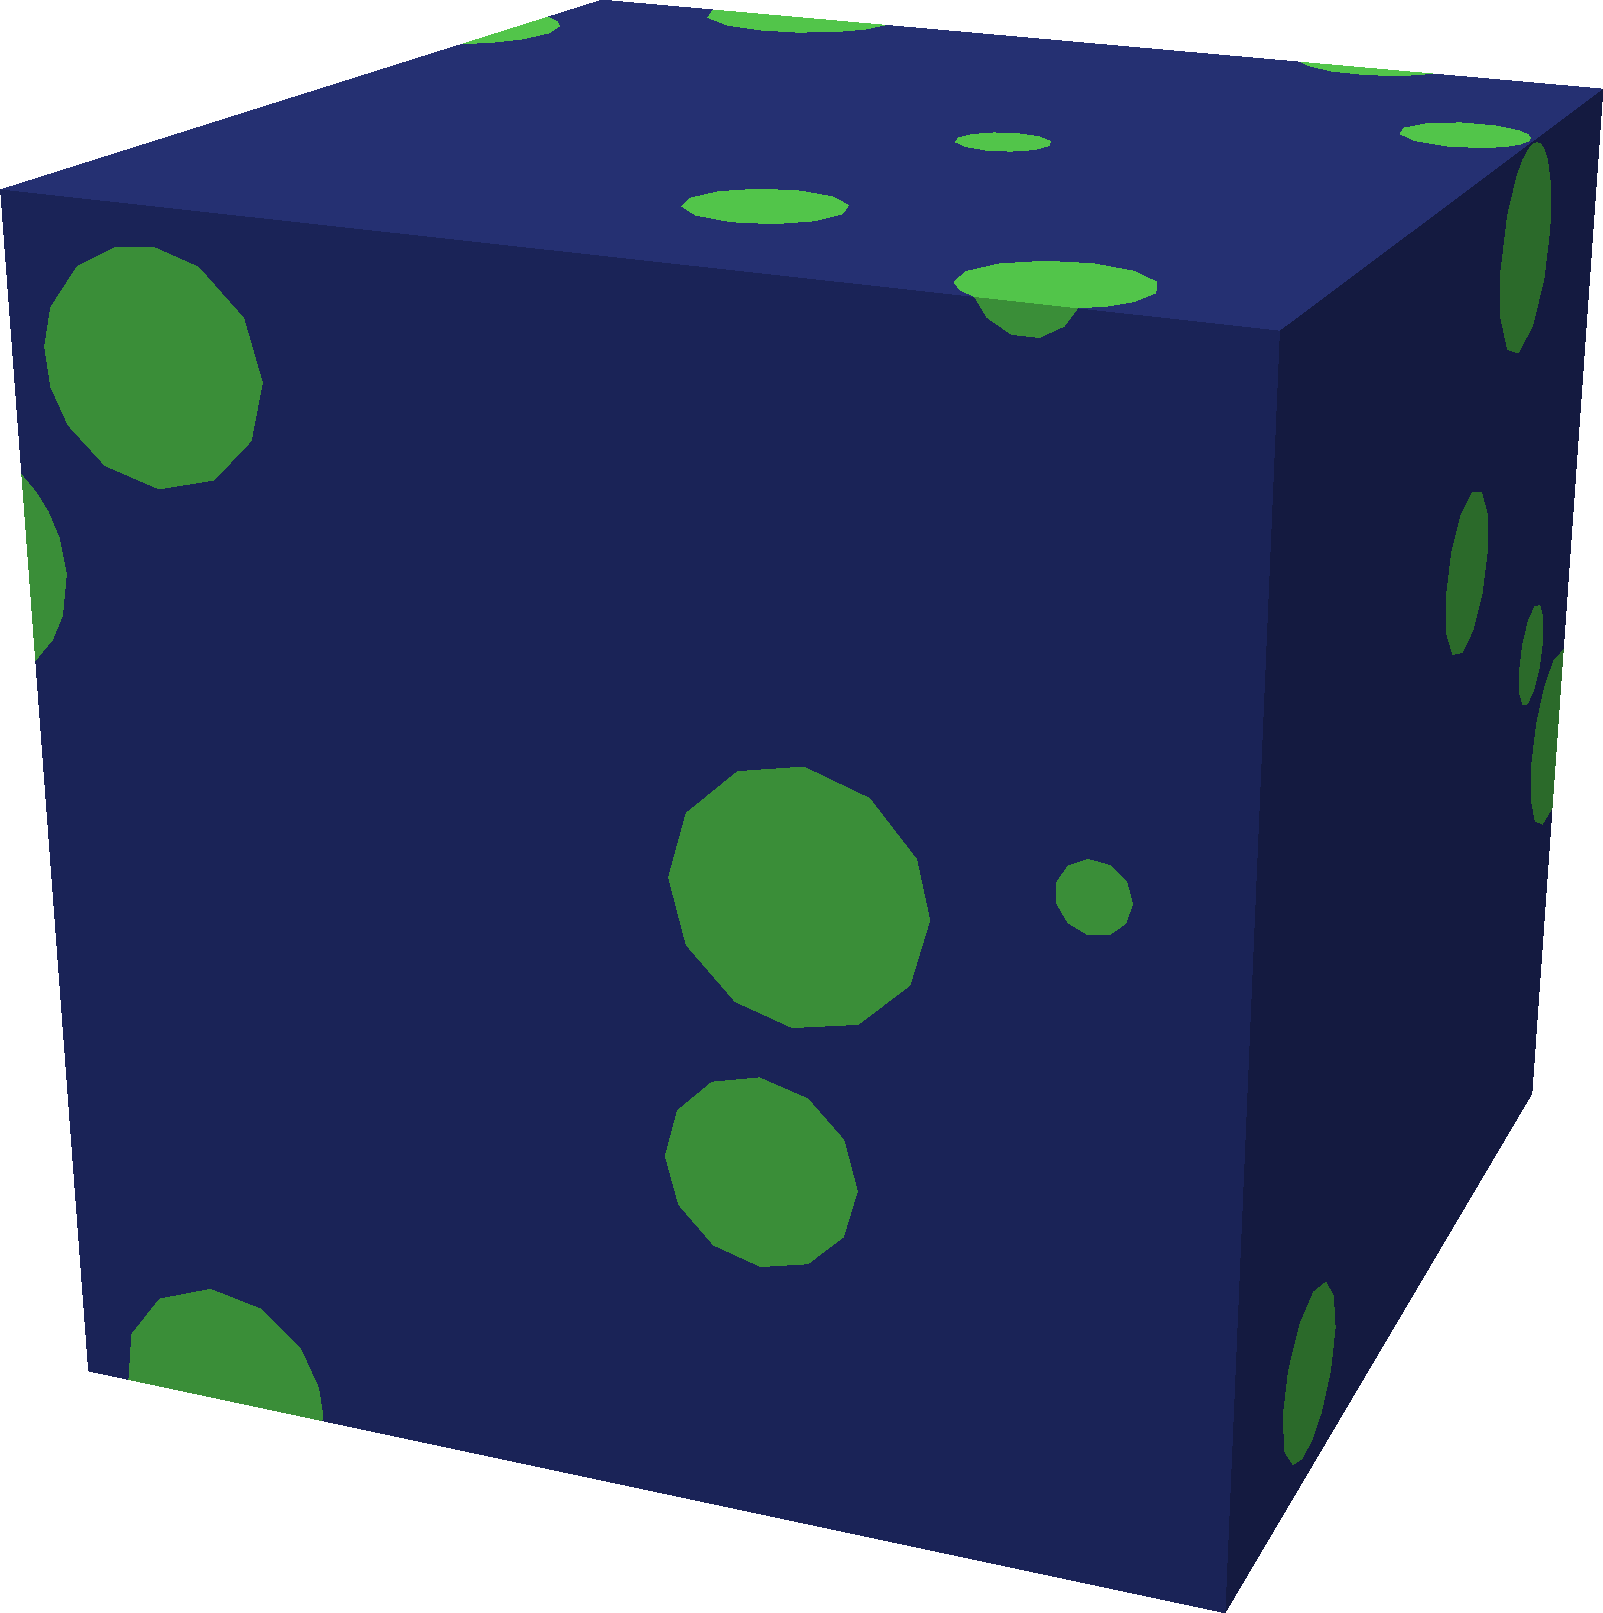
\includegraphics[width=0.4\linewidth]{rve6.png}
 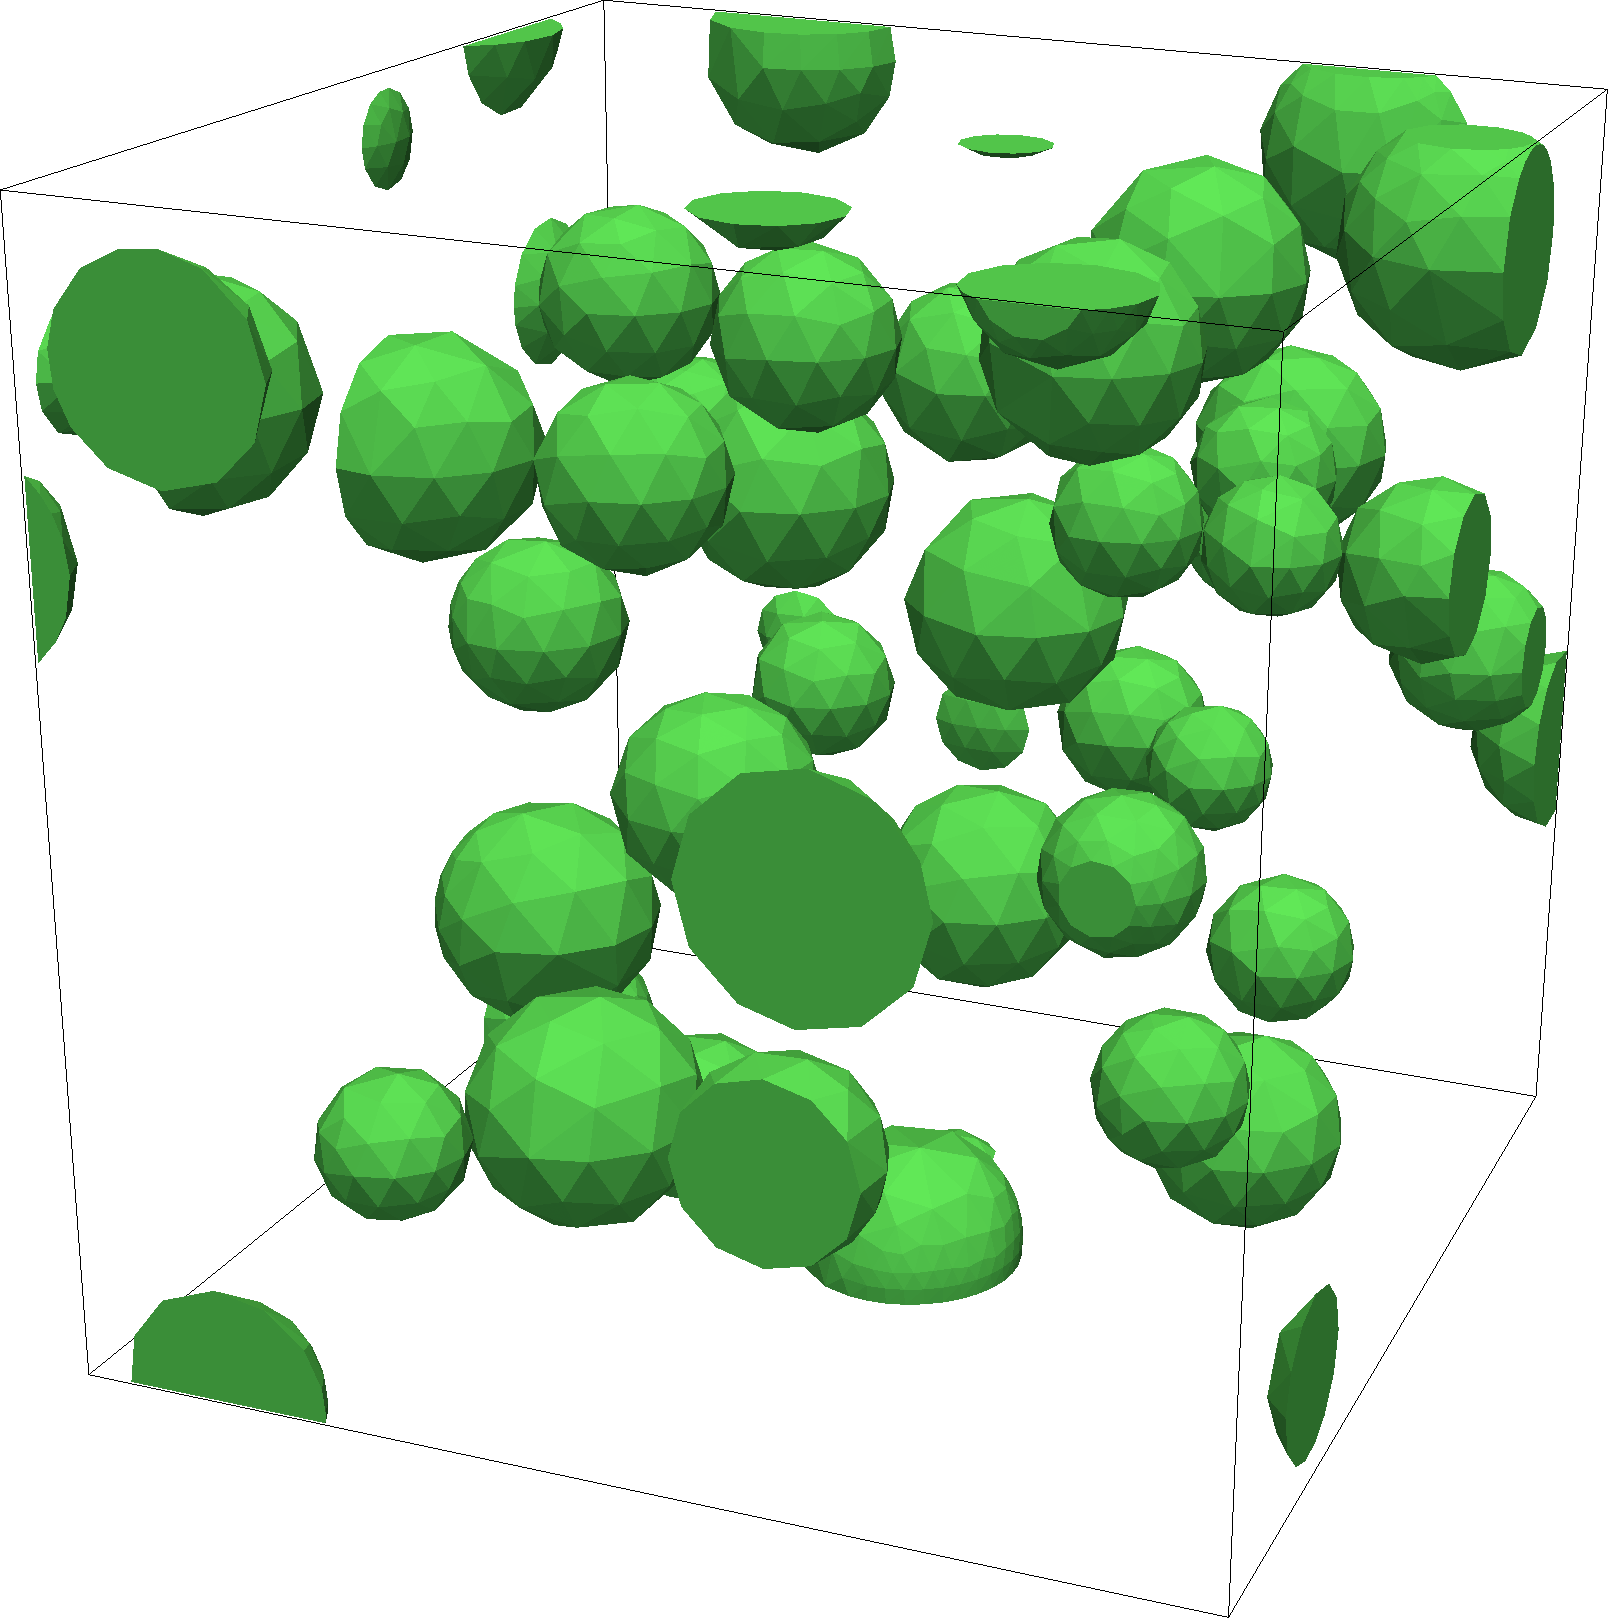
\includegraphics[width=0.4\linewidth]{rve6_inc.png}
\caption{\csentence{SVE-cube with sample realization of particle composite of size $6\times 6\times 6$.}\label{fig:rve_sample6}}
\end{figure}

\begin{figure}[htb]
\centering
 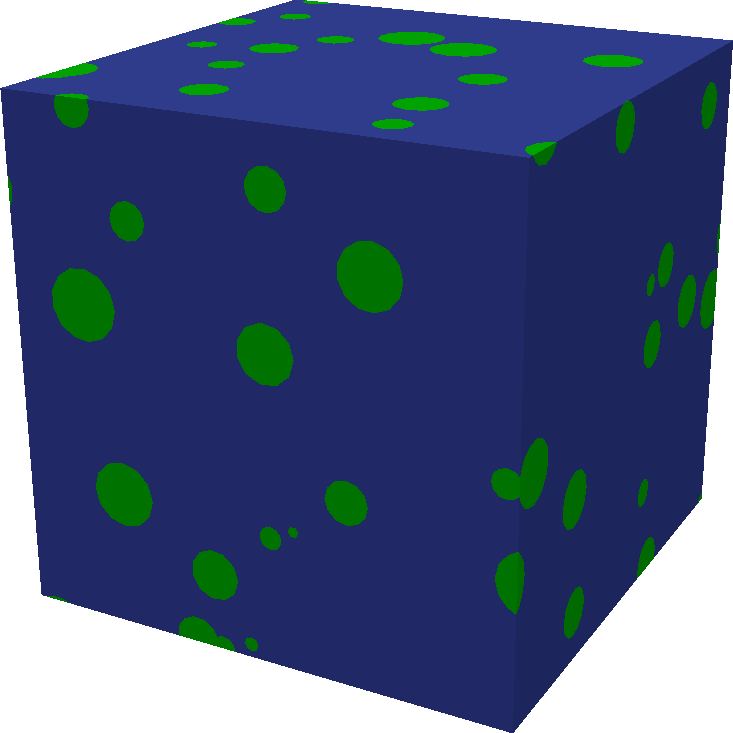
\includegraphics[width=0.4\linewidth]{rve9.png}
 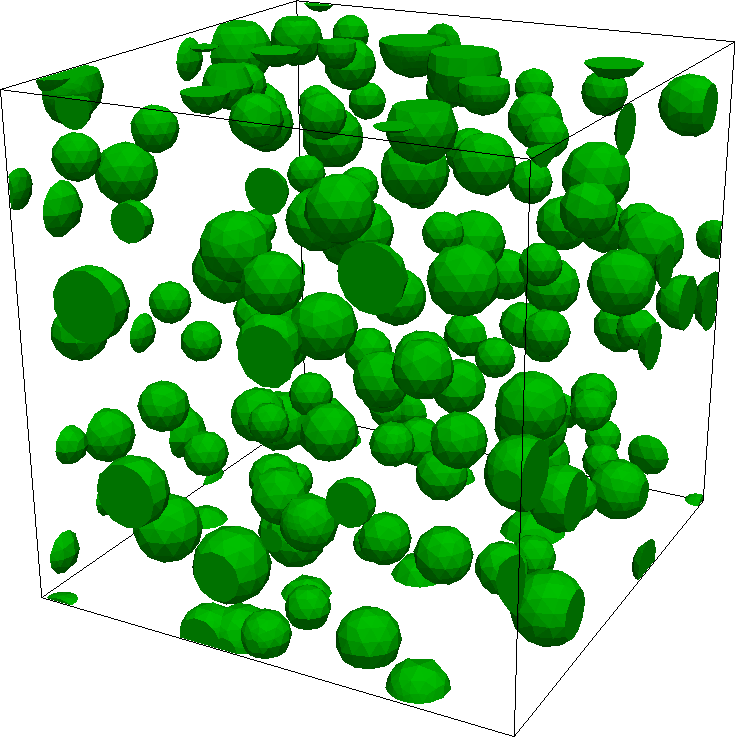
\includegraphics[width=0.4\linewidth]{rve9_inc.png}
\caption{\csentence{SVE-cube with sample realization of particle composite of size $9\times 9\times 9$.}\label{fig:rve_sample9}}
\end{figure}

\begin{figure}[htb]
\centering
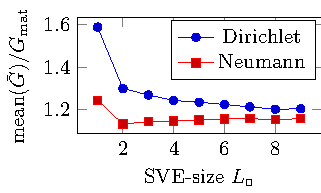
\includegraphics{meanG}
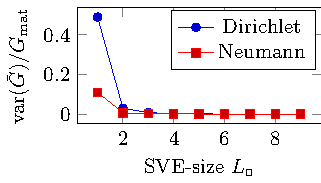
\includegraphics{varG}
\caption{\csentence{Statistical comparison of the influence of the boundary conditions (Dirichlet, Neumann) on the macroscale shear modulus, $\bar{G}$.}}
\label{fig:SVE_comp}
\end{figure}

\begin{figure}[htb]
\centering
 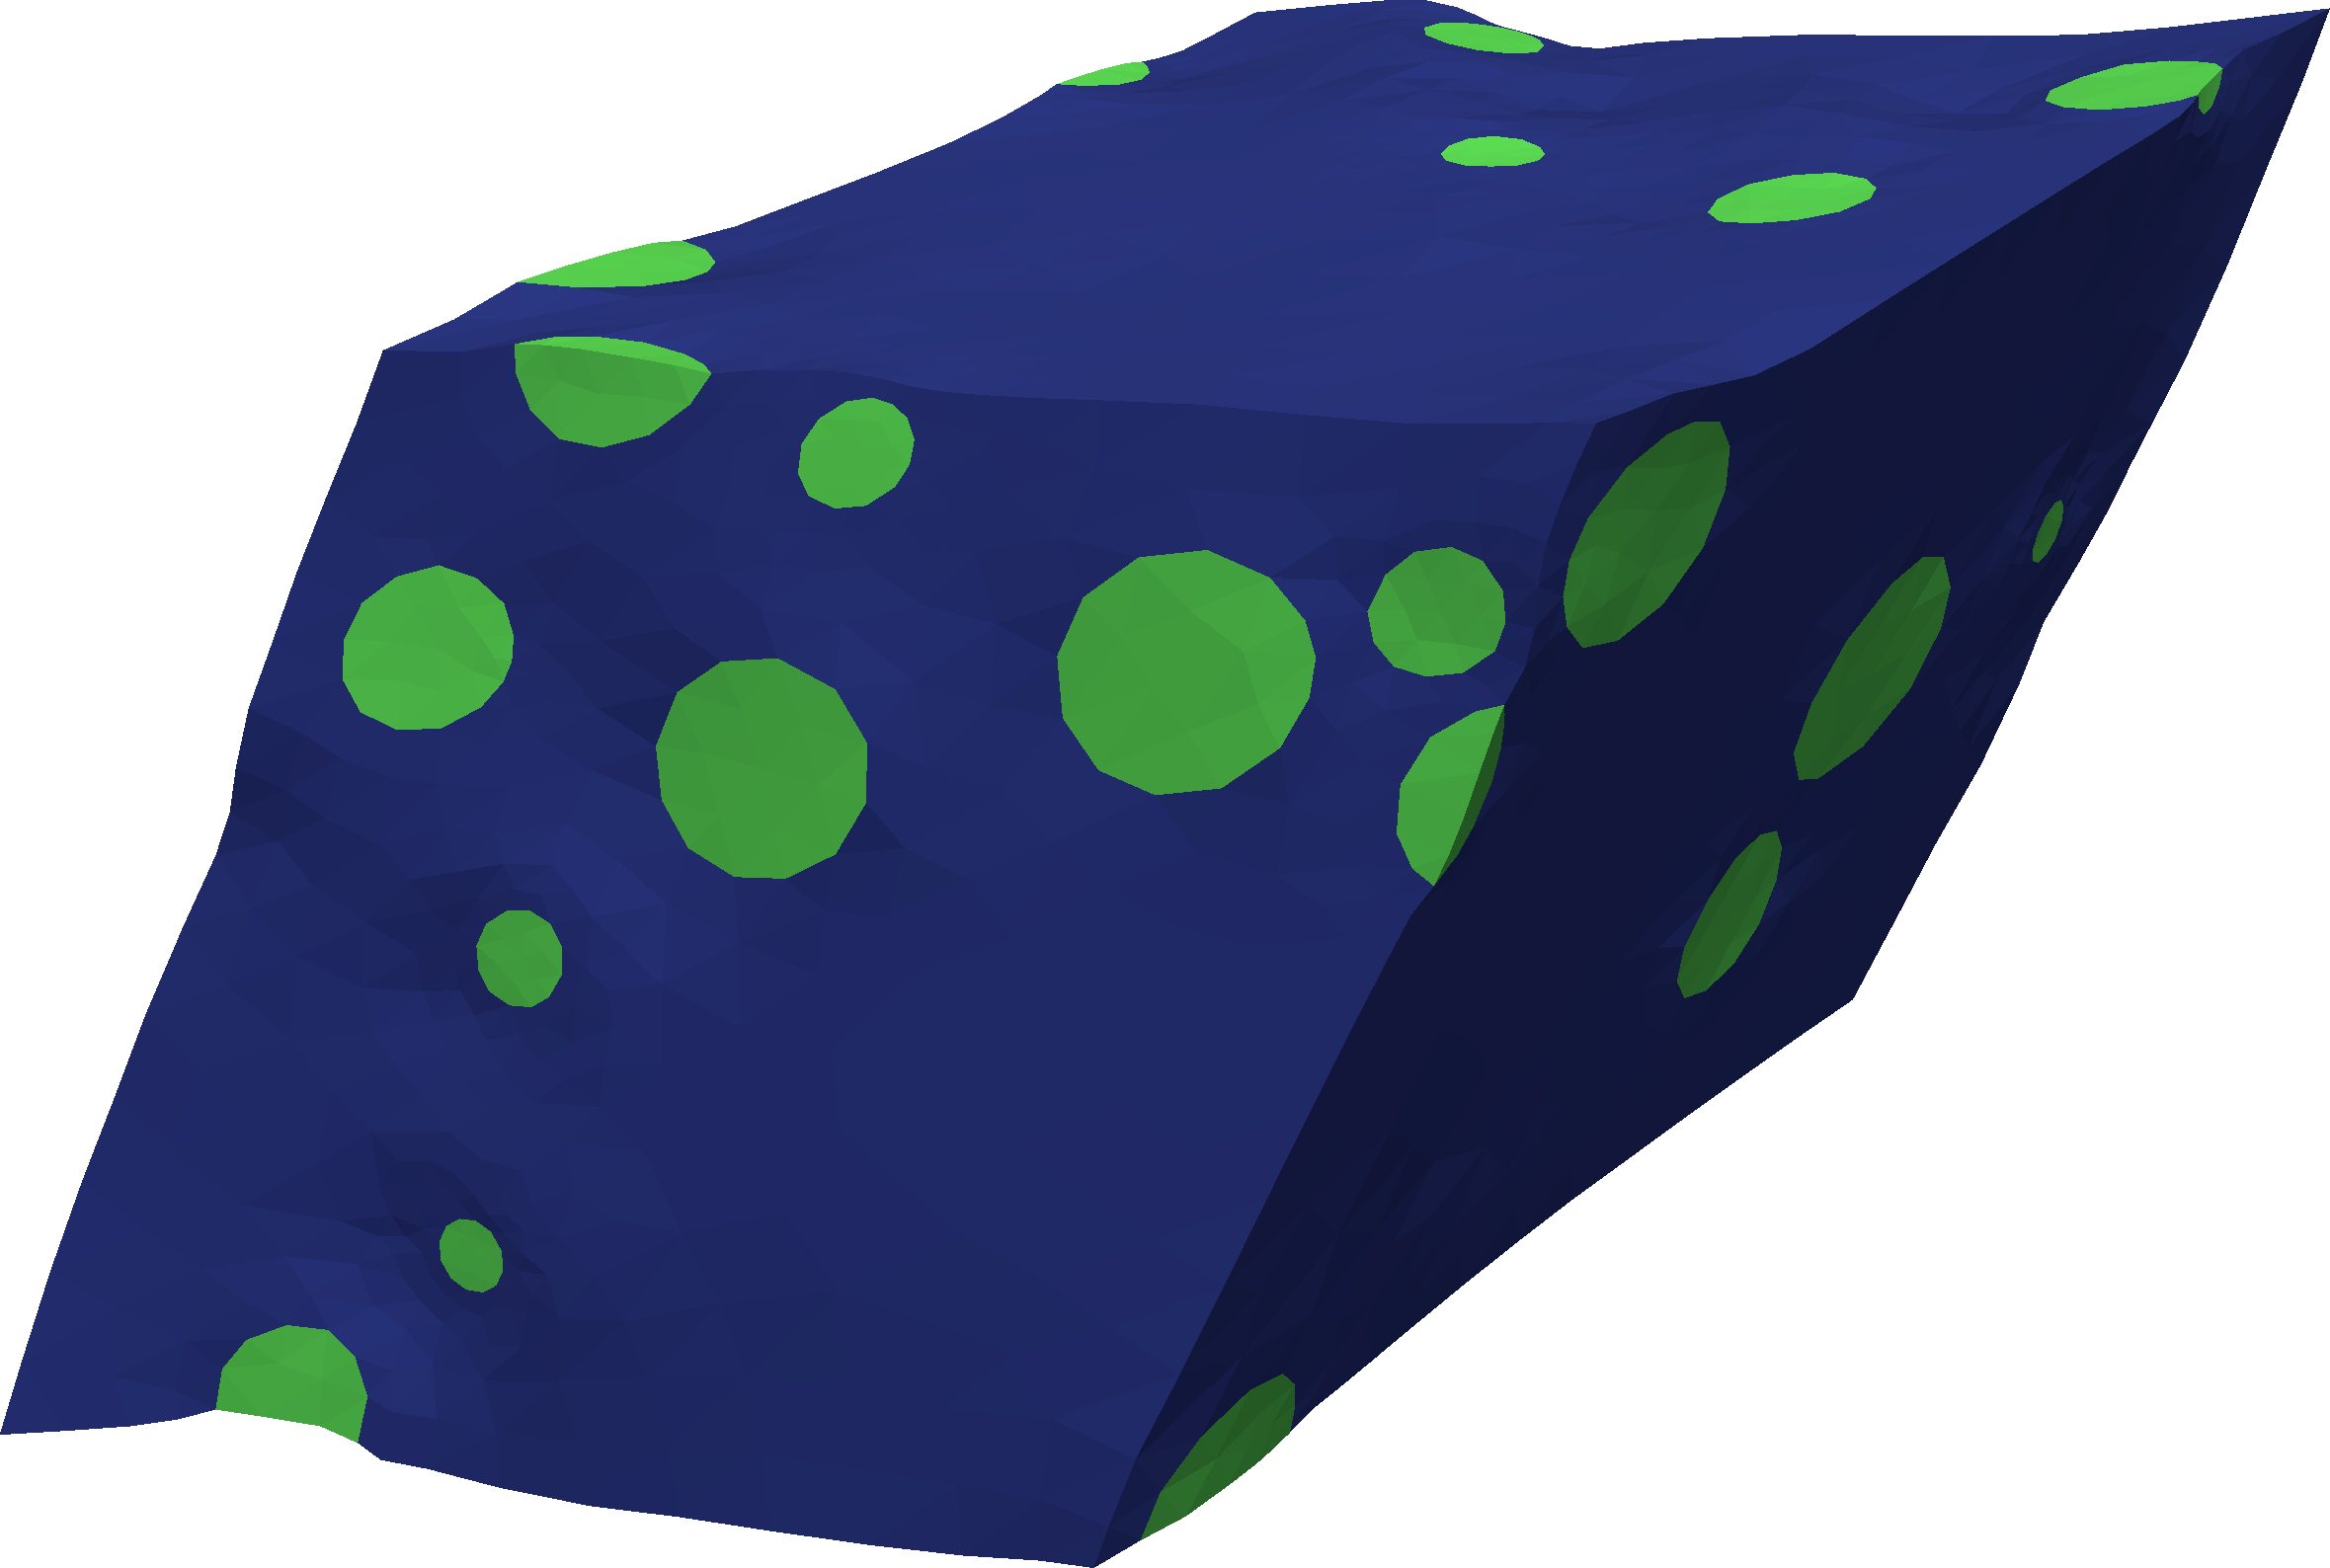
\includegraphics[width=0.5\linewidth]{rve6_def.png}
\caption{\csentence{A sample SVE subjected to macroscopic pure shear}. The prescribed macroscopic shear is $(\bar{\ts\epsilon}_\dev)_{ij} = 0.4[1 - \delta_{ij}]$.}
\label{fig:def_rve6}
\end{figure}

\begin{figure}[htbp!]
\centering
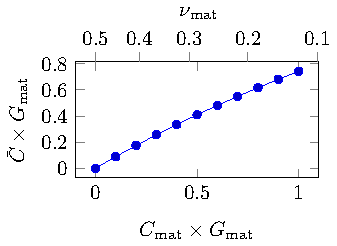
\includegraphics{CGmat}
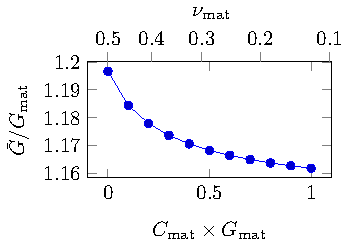
\includegraphics{GGmat}
\caption{\csentence{Homogenized results from a single RVE with Dirichlet boundary condition.}
Dependence of effective properties $\bar{C}$ and $\bar{G}$ on the bulk compliance $C_\mathrm{mat}$ for fixed values of $G_\mathrm{part} = 5\,G_\mathrm{mat}$ and $C_\mathrm{part} = 0$.}
\label{fig:RVE_compressibility}
\end{figure}

%%%%%%%%%%%%%%%%%%%%%%%%%%%%%%%%%%%
%%                               %%
%% Tables                        %%
%%                               %%
%%%%%%%%%%%%%%%%%%%%%%%%%%%%%%%%%%%

%% Use of \listoftables is discouraged.
%%
% \section*{Tables}
% \begin{table}[h!]
% \caption{Sample table title. This is where the description of the table should go.}
%       \begin{tabular}{cccc}
%         \hline
%            & B1  &B2   & B3\\ \hline
%         A1 & 0.1 & 0.2 & 0.3\\
%         A2 & ... & ..  & .\\
%         A3 & ..  & .   & .\\ \hline
%       \end{tabular}
% \end{table}

%%%%%%%%%%%%%%%%%%%%%%%%%%%%%%%%%%%
%%                               %%
%% Additional Files              %%
%%                               %%
%%%%%%%%%%%%%%%%%%%%%%%%%%%%%%%%%%%

% \section*{Additional Files}
%   \subsection*{Additional file 1 --- Sample additional file title}
%     Additional file descriptions text (including details of how to
%     view the file, if it is in a non-standard format or the file extension).  This might
%     refer to a multi-page table or a figure.
% 
%   \subsection*{Additional file 2 --- Sample additional file title}
%     Additional file descriptions text.


\end{backmatter}
\end{document}
